\newcommand{\microns}{$\upmu$m\xspace}
\newcommand{\etal}{\textit{et al.}\xspace}
\newcommand{\Ef}{$E_{F}$\xspace}
\newcommand{\SiO}{SiO$_{2}$\xspace}
\newcommand{\insitu}{\textit{in situ}\xspace}
\newcommand{\Ohms}{$\Omega$\xspace}

\newcommand{\InsertFig}[3]{
  \begin{figure}[!htbp]
    \begin{center}
      \leavevmode
      #1
      \caption{#2}
      \label{#3}
    \end{center}
  \end{figure}
}




\documentclass[twoside,11pt]{Classes/myThesis}


%%%%%%%%%%%%%%%%%%%%%%%%%%%%%%%%%%%%%%%%%%%%%%%%%%%%%%
%%%%%%%%%%%%%%% file path for figures - add extra chapters as necessary %%%%%%%%%
%%%%%%%%%%%%%%%%%%%%%%%%%%%%%%%%%%%%%%%%%%%%%%%%%%%%%%
\graphicspath{{./Chapters/Chapter_1/Chapter_1_Fig/}     
              {./Chapters/Chapter_2/Chapter_2_Fig/}
              {./Chapters/Chapter_2a/Chapter_2a_Fig/}
              {./Chapters/Chapter_2b/Chapter_2b_Fig/}
              {./Chapters/Chapter_3/Chapter_3_Fig/}
              {./Chapters/Chapter_4/Chapter_4_Fig/}
              {./Chapters/Chapter_5/Chapter_5_Fig/}
              {./Appendix1/Appendix1_Fig/}
              {./ThesisFigs/}}

%%%%%%%%%%%%%%%%%%%%%%%%%%%%%%%%%%%%%%%%%%%%%%%%%%%%%%
%%%%%%%%%%%%% Constants - fill these in for use throughout the thesis %%%%%%%%%%%%
%%%%%%%%%%%%%%%%%%%%%%%%%%%%%%%%%%%%%%%%%%%%%%%%%%%%%%
\newcommand{\theAuthor}{Rodrigo Daniel Solis Ortega}
\newcommand{\authorEmail}{el14rdso@leeds.ac.uk}
\newcommand{\myTitle}{Modelling and characterization of soft materials for bioinspired series-elastic actuators}
%%%%%%%%%%%%%%%%%%%%%%%%%%%%%%%%%%%%%%%%%%%%%%%%%%%%%%
\pdfinfo { /Title  (\myTitle)
           /Creator (TeX)
           /Producer (pdfTeX)
           /Author (\theAuthor \authorEmail)
           /ModDate (D:\pdfdate)
           /CreationDate (D:\pdfdate)  %format D:YYYYMMDDhhmmss
           /Subject (Condensed Matter Physics)
           /Keywords (PhD, Thesis)}    
		\pdfcatalog { /PageMode (/UseOutlines)
                  /OpenAction (fitbh)  }

%%%%%%%%%%%%%%%%%%%%%%%%%%%%%%%%%%%%%%%%%%%%%%%%%%%%%%
%%%%%%%%%%%%% Title Page Information %%%%%%%%%%%%%%%%%%%%%%%%%%%%
%%%%%%%%%%%%%%%%%%%%%%%%%%%%%%%%%%%%%%%%%%%%%%%%%%%%%%
\title{\myTitle}
\author{\href{mailto:\authorEmail}{\theAuthor}}
\crest{
\includegraphics[width=35mm]{Leeds_Crest.png}}
%%%%%%%%%%%%%%%%%%%%%%%%%%%%%%%%%%%%%%%%%%%%%%%%%%%%%%
%% Define these as empty to omit the two logos on the title page
%%%%%%%%%%%%%%%%%%%%%%%%%%%%%%%%%%%%%%%%%%%%%%%%%%%%%%
\logo{\includegraphics[width=50mm]{UoL_logo}} %University Logo
\deptlogo{} %\includegraphics[width=50mm]{UoL_logo}} % Institute Logo
%%%%%%%%%%%%%%%%%%%%%%%%%%%%%%%%%%%%%%%%%%%%%%%%%%%%%%
\collegeordept{\href{https://engineering.leeds.ac.uk/mechanical}{Institute of Design, Robotics and Optimization \\* School of Mechanical Engineering}}
\university{\href{http://www.leeds.ac.uk}{University of Leeds}}

\degree{Doctor of Philosophy}
\degreedate{\monthdate\today}

%Different font in caption
%%%%%%%%%%%%%%%%%%%%%%%%%%%%%%%%%%%%%%%%%%%%%%%%%%%%%%
%%%%%%%%%%%%%%%% Optional Packages  %%%%%%%%%%%%%%%%%%%%%%%%%%%
%%%%%%%%%%%%%%%%%%%%%%%%%%%%%%%%%%%%%%%%%%%%%%%%%%%%%%
%\usepackage{StyleFiles/watermark}
\usepackage{xspace}  %add a space after maths if not already there
%\usepackage{booktabs} %better tables
%\usepackage{rotating}  %rotating figures and tables
\usepackage{array} %enhanced tables
%\usepackage{ctable} %include a figure command
%\usepackage{footnote}
\usepackage{multirow} %for merging cells on tables
%\usepackage{times} % The "Times" font
%\usepackage{Utopia} % The "Utopia" font
\usepackage[toc,page]{appendix}
\usepackage{caption}
\usepackage{subcaption} %This solve the error caused with subfigure
\usepackage{float}
\usepackage{hyperref}
\usepackage[ruled,vlined]{algorithm2e}
\usepackage{cleveref}
\usepackage[ruled,vlined]{algorithm2e}
\usepackage{enumitem}
\usepackage{rotating}
\usepackage{booktabs}
\newcommand{\ra}[1]{\renewcommand{\arraystretch}{#1}}
%User Definitions
\newcolumntype{C}[1]{>{\centering\arraybackslash}p{#1}}

\linespread{1.3} %1.5 line spacing

\begin{document}

\maketitle

%set the number of sectioning levels that get number and appear in the contents
\setcounter{secnumdepth}{3}
\setcounter{tocdepth}{3}
%Make the label printed by autoref be section for subsection and subsubsection
\let\subsectionautorefname\sectionautorefname
\let\subsubsectionautorefname\sectionautorefname
\pagenumbering{roman}
\frontmatter

%Insert empty page after title
\newpage\null\thispagestyle{empty}\newpage

%%%%%%%%%%%%%%%%%%%%%%%%%%%%%%%%%%%%%%%%%%%%%%%%%%%%%%
%%%%%%%%%%%% Include sections are required, or comment out to skip over %%%%%%%%%
%%%%%%%%%%%%%%%%%%%%%%%%%%%%%%%%%%%%%%%%%%%%%%%%%%%%%%
%% Thesis Dedictation ---------------------------------------------------

\begin{dedication} %this creates the heading for the dedication page

This thesis is dedicated to someone.

\end{dedication}

% ----------------------------------------------------------------------

%%% Local Variables: 
%%% mode: latex
%%% TeX-master: "../thesis"
%%% End: 

% Thesis IP Statement ---------------------------------------------------

\begin{ipstatement}
The candidate confirms that the work submitted is his own, except where work which has formed part of jointly authored publications has been included. The contribution of the candidate and the other authors to this work has been explicitly indicated below. The candidate confirms that appropriate credit has been given within the thesis where reference has been made to the work of others.
\\
\\
\hyperref[sec:characterizationKKP]{Section~\ref*{sec:characterizationKKP}} of this thesis is based on a jointly-authored conference paper: \textit{Solis-Ortega, R.D., Dehghani-Sanij, A.A. and Martinez-Hernandez, U., 2017, July. Characterization of kinetic and kinematic parameters for wearable robotics. In Annual Conference Towards Autonomous Robotic Systems (pp. 548-556). Springer, Cham.}.
\\
\\
Section X.X of this thesis is based on a jointly-authored conference paper: \textit{Solis-Ortega, R.D., Dehghani-Sanij, A.A. and Martinez-Hernandez, U., 2018, August. The assessment of viscoelastic models for nonlinear soft materials. In 2018 7th IEEE International Conference on Biomedical Robotics and Biomechatronics (Biorob) (pp. 1274-1279). IEEE.}.
\\
\\
The contributions of the candidate to these papers include the literature review, data collection, design and execution of simulation, statistical analysis, and writing. The contribution of the other authors to these papers include guidance, supervision, and revision.
\\
\\
This copy has been supplied on the understanding that it is copyright material and that no quotation from the thesis may be published without proper acknowledgement.
\\
\\
The right of \theAuthor{} to be identified as Author of this work has been asserted by him in accordance with the Copyright, Designs and Patents Act 1988.
\\
\\
\copyright{} \yeardate{\today} The University of Leeds and \theAuthor{}.

\label{ips}
\end{ipstatement}

% ----------------------------------------------------------------------

%%% Local Variables: 
%%% mode: latex
%%% TeX-master: "../thesis"
%%% End: 

% Thesis Acknowledgements ------------------------------------------------


%\begin{acknowledgementslong} %uncommenting this line, gives a different acknowledgements heading
\begin{acknowledgements}      %this creates the heading for the acknowlegments

\setlength{\parindent}{17.62482pt}
\setlength{\parskip}{0.0pt plus 1.0pt}

\textit{I would like to thank to both Professor Abbas Dehghani-Sanji and Dr Uriel Martinez Hernandez who have guided me throughout this far on the pursue of a PhD. As well as the many people who directly or indirectly were involved in this personal goal. I would like to thank my family for always being extremely supporting and to my financial sponsor CONACYT.}

\end{acknowledgements}
%\end{acknowledgmentslong}

% ------------------------------------------------------------------------

%%% Local Variables: 
%%% mode: latex
%%% TeX-master: "../thesis"
%%% End: 


% Thesis Abstract -----------------------------------------------------


%\begin{abstractslong}    %uncommenting this line, gives a different abstract heading
\begin{abstracts}        %this creates the heading for the abstract page

\setlength{\parindent}{17.62482pt}
\setlength{\parskip}{0.0pt plus 1.0pt}
	
This emerging field of soft robotics is currently being applied for human assistance applications such as soft orthoses or soft exosuits able to assist human movements. The elder people is main sector of the population which will be directly benefited by the development of a portable, compliant, lightweight and efficient soft exosuit. Current developments rely on well established technologies such as pneumatic artificial muscles and electric motors paired with Bowden cables. However, many research is aiming on improving both the established technologies and emerging technologies such as shape memory materials. The current report describes the state of the mentioned field of interest while paying particular attention to the soft actuation technologies advantages, limitations and proposed improvements. In a similar way, the soft perception technology is as well discussed along the control techniques being implement-ed in soft exosuits and soft orthoses. Furthermore, the development of a hybrid soft actuator is proposed by combining two or more available technologies in an attempt to overcome their individual limitations. Moreover, as a preliminary design step, it is described the characterization of the parameters for the human lower limb for daily living activities which aims to provide the information required to tailor the hybrid soft actuator design parameters. The characterization considers four main daily activities: walking, using steps, walking on a ramp and using a chair. In the same way, the parameters of torque, angle and power during such activities were recorded from several clinical trials and plotted for analyzing. Through the obtained charts it is possible to define the required parameters of the soft hybrid actuator to be designed. Finally, as a preliminary experimental work, the feasibility of imitating the musculoskeletal-tendon system is assessed by characterizing the mechanical properties of polyethylene rubber, since the literature suggest that this type of material have similar properties as the human tendon.

\end{abstracts}
%\end{abstractlongs}

% ----------------------------------------------------------------------

%%% Local Variables: 
%%% mode: latex
%%% TeX-master: "../thesis"
%%% End: 

\tableofcontents
\listoffigures
\let\cleardoublepage\clearpage
\listoftables
\let\cleardoublepage\clearpage
\begin{abbreviations}
%Place your abbreviations in here...

% Table generated by Excel2LaTeX from sheet 'abbr'

\begin{table}[h]
\centering
\small{
\begin{tabular}{lp{5cm}llp{5cm}ll}
AC    & Alternating Current &       & PCAR   & Point Contact Andreev Reflections \\
BCS   & Bardeen-Cooper-Schrieffer &       & MR    & Magnetoresistance \\
DC    & Direct Current &      & FET   & Field Effect Transistor  \\       
FWHM  & Full Width Half Maximum &      & UHV   & Ultra High Vacuum \\
\end{tabular}
}
\label{tbl:Abbreviations}
\end{table}

%\begin{table}[here]
%\centering
%\begin{tabular}{ll}
%
%2DEG & Two Dimensional Electron Gas\\
%AC & Alternating Current\\
%AR & Andreev Reflection \\
%BCS & Bardeen-Cooper-Schrieffer\\
%BLG & Bi-Layer Graphene\\
%CCD & Charge Coupled Device \\
%CNP & Charge Neutrality Point\\
%CVD & Chemical Vapour Deposition\\
%DAC & Digital-to-Analogue Converter\\
%DC & Direct Current\\
%DFT & Density Functional Theory \\
%EBL & Electron Beam Lithography\\
%EFE & Electric Field Effect\\
%FET & Field Effect Transistor\\
%FLG & Few Layer Graphene\\
%FWHM & Full Width Half Maximum\\
%h-BN & hexagonal Boron Nitride\\
%IPA & Isopropyl Alcohol \\
%JJ & Josephson Junction\\
%MAR & Multiple Andreev Reflections\\
%MIBK & Methyl Isobutyl Ketone\\
%MR & Magnetoresistance\\
%OL & Optical Lithography \\
%PMMA & Poly(Methyl Meth-Acrylate)\\
%QHE & Quantum Hall Effect\\
%SdHO & Shubnikov de-Haas Oscillation\\
%SEM & Scanning Electron Microscope\\
%SGS & Superconductor-Graphene-Superconductor\\
%SIS & Superconductor-Insulator-Superconductor\\
%SLG & Single Layer Graphene\\
%SNS & Superconductor-Normal-Superconductor\\
%SPCM & Scanning Photo-Current Microscopy\\
%TK & Tuinstra-Koenig\\
%TLM & Transfer Length Measurement\\
%UHV & Ultra High Vacuum\\
%VTI & Variable Temperature Insert\\
%
%\end{tabular} 
%\label{tbl:Abbreviations}
%\end{table}

%$V_{D}$ & Dirac Point voltage \\
%$V_{g}$  & Gate voltage\\
%$E_{F}$ & Fermi Energy\\
%$v_{f}$ & Fermi velocity \\
%$\omega_{c}$ & Cyclotron Frequency \\
%%$k_{B}$  & Boltzmann's constant \\
%T_{c}

\end{abbreviations}

\begin{Common_Symbols}
%Place your abbreviations in here...

% Table generated by Excel2LaTeX from sheet 'abbr'

\begin{table}[h]
\centering

\begin{tabular}{ll}

$B$   & Applied Magnetic Field ($\mu_{0}H$) \\
$\Delta$ & Superconducting Gap Parameter \\
\Ef & Fermi Energy \\
$e$   & Elementary Charge \\
$\epsilon_{0}$ & Permittivity of Free Space \\
$h$   & Planck's Constant \\
$\hbar$ & $h/2\pi$ \\
$I_{c}$ & Critical Current \\
$\mu$ & Carrier Mobility \\
$n_{s}$ & Carrier Density \\
$\omega_{c}$ & Cyclotron Frequency \\
$\rho$ & Resistivity \\
$\sigma$ & Conductivity \\
$T$ & Temperature \\
$T_{c}$ & Critical Temperature \\
$v_{F}$ & Fermi Velocity 
\end{tabular}

\label{tbl:Common_Symbols}
\end{table}

%\begin{table}[here]
%\centering
%\begin{tabular}{ll}
%
%2DEG & Two Dimensional Electron Gas\\
%AC & Alternating Current\\
%AR & Andreev Reflection \\
%BCS & Bardeen-Cooper-Schrieffer\\
%BLG & Bi-Layer Graphene\\
%CCD & Charge Coupled Device \\
%CNP & Charge Neutrality Point\\
%CVD & Chemical Vapour Deposition\\
%DAC & Digital-to-Analogue Converter\\
%DC & Direct Current\\
%DFT & Density Functional Theory \\
%EBL & Electron Beam Lithography\\
%EFE & Electric Field Effect\\
%FET & Field Effect Transistor\\
%FLG & Few Layer Graphene\\
%FWHM & Full Width Half Maximum\\
%h-BN & hexagonal Boron Nitride\\
%IPA & Isopropyl Alcohol \\
%\Vg & Gate Voltage \\
%JJ & Josephson Junction\\
%MAR & Multiple Andreev Reflections\\
%MIBK & Methyl Isobutyl Ketone\\
%MR & Magnetoresistance\\
%OL & Optical Lithography \\
%PMMA & Poly(Methyl Meth-Acrylate)\\
%QHE & Quantum Hall Effect\\
%SdHO & Shubnikov de-Haas Oscillation\\
%SEM & Scanning Electron Microscope\\
%SGS & Superconductor-Graphene-Superconductor\\
%SIS & Superconductor-Insulator-Superconductor\\
%SLG & Single Layer Graphene\\
%SNS & Superconductor-Normal-Superconductor\\
%SPCM & Scanning Photo-Current Microscopy\\
%TK & Tuinstra-Koenig\\
%TLM & Transfer Length Measurement\\
%UHV & Ultra High Vacuum\\
%VTI & Variable Temperature Insert\\
%
%\end{tabular} 
%\label{tbl:Abbreviations}
%\end{table}

%$V_{D}$ & Dirac Point voltage \\
%$V_{g}$  & Gate voltage\\
%$E_{F}$ & Fermi Energy\\
%$v_{f}$ & Fermi velocity \\
%$\omega_{c}$ & Cyclotron Frequency \\
%%$k_{B}$  & Boltzmann's constant \\
%T_{c}

\end{Common_Symbols}


\mainmatter

\pagenumbering{arabic}
\chapter{Introduction}
\section{ Background}

\Large{The background must give an overview of the current development, the progress of the research and the gaps in knowledge (research opportunities) }

The field of Soft robotics deals with the implementation of soft and deformable materials in traditional Robotics applications. The interest and research in this field has increased in the past decade. The latter is due to the outstanding developments in terms of manufacturing of soft materials, such as elastomers, and the development of new soft materials which can be stimulated, i.e. deformed, by heat, light, and magnetism. 

The coordination action called RoboSoft, supported by the IEEE Robotics and Automation Society (RAS) and the European Commission, has played a very important role in spreading the awareness of the wide number of Soft Robotics applications. The RoboSoft committee formally defines the field of Soft Robotics as ``Soft robot/devices that can actively interact with the environment and can undergo `large' deformations relying on inherent or structural compliance'' \cite{laschi2016soft}. The categorization of when a robotic application fall into the field of Soft Robotics depends on the material's Young Modulus, a mechanical property which relates the material's deformation with the amount of stress applied to it; which must be between the range of 10$^{2} - $10$^{6}$ Pascals (Pa). The Young's modulus is usually a measure of a solid material stiffness; a high value refers to a stiff material in the same way as a low value refers to an elastic or soft material. In the context of Soft Robotics, the term compliance it is most used instead of stiffness since it refers to the adaptability of the material under certain circumstances.

Early applications in Soft Robotics were inspired in nature, by observing that most biological organisms are not rigid, e.g. the human skeleton only contributes with 11\% of an adult's weight, on contrast, the skeletal muscle in our body only contributes with 42\% of the weight \cite{kim2013soft}. This inspiration gave birth to several soft bio-inspired robots, as well as the interest in studying the embodied intelligence of biological organisms. The latter refers to the ability of biological organisms to adapt to different situations by exploding their body morphology and properties. This is one of the main differences between soft and rigid robots. The embodied intelligence of soft robots release the controller from the task of accurately controlling the position of the robot and of constantly monitoring the working environment; allowing the controller to focus on the execution of commands. This is only possible with the implementation of soft and deformable materials able to automatically adapt to perturbations from the environment, such as uneven terrains and obstacles. Bio-inspired soft robots are now being developed for a broad range of applications, such as locomotion, manipulation, and even replicating biological processes such as digestion. The research done in the field of Soft Robotics has an interesting multidisciplinary potential. For example, the locomotion of caterpillars and snake could be study by building a soft robot which replicates this motion. The knowledge extracted from this could be useful for the development of actuated bendable soft cylinders which ultimately could replace the current rigid tools being used in laparoscopic surgery \cite{rus2015design}.

The mechanical behaviour of soft materials, is very difficult to model using traditional mathematical models, due to their non-linear, time-dependent and strain-rate-dependent stress response. This great challenge motivated the research in Soft Robotics to develop bio-inspired soft bodies, arms and legs able to perform the task at hand using minimal control. This caused a shift in the traditional design approach for rigid robots from ``rigidity by design, safety by sensors and control'' to design approach used in soft robots, ``safety by design, performance by control''. The added feature of safety, inherent in most soft robots, allowed the development of Physical Human-Robot Interaction (PHRI) applications \cite{filippini2008toward}. Many other challenges face by this emerging field are listed in \cite{laschi2016soft,trivedi2008soft} being: actuation of soft materials, development and implementation of soft sensors into soft robots, control systems able to deal with the nonlinear behaviour of soft materials, and modelling tools able to accurately predict the mechanical behaviour of soft materials in real-time. Most of these limitations come from the simple fact that soft robots cannot be considered as a chain of rigid links able to rotate or slide as common robots are, but soft robots are deformable and continuous which means that all the foundation in which Robotics is based on, is not easily transferable to the Soft Robotics field. 

The design and development of soft robots is very challenging, however, the potential benefits are many \cite{iida2011soft}. Foe example, soft robots have the potential of being very dexterous due to the ability of modifying their shape depending on the environment; soft robots can can manipulate objects of different shapes, sizes, and most importantly they are safe to interact with humans in the event of an unplanned collision. The latter benefits highlight the potential of Soft Robotics for PHRI applications such as, orthoses, surgical tools, and wearable devices. This research aims to contribute to the technological advance of Soft Robotics for human assistance applications.

For a long time, humans have pursued the idea of increasing their strength, stamina and speed through different means. Currently, we are relaying on technological advances to achieve the latter by building wearable robotic devices, commonly known as robotic exoskeletons. This wearable device was motivated by military applications where a soldier is required to carry a heavy load in its back for a long period of time, ultimately causing him injuries or early fatigue. The robotic exoskeleton is able to carry a payload and transmit the payload weight to the ground, ideally relieving the wearer from feeling the payload, which allows the wearer to walk greater distances without premature fatigue. The rigid nature of these devices and the big actuators implemented to achieve forces able to enhance humans, impose many limitations, such as, restriction of body movements, interference on subject natural biomechanics and high inertia which impedes the device to follow the subject intentions smoothly, creating a drag feeling \cite{asbeck2014stronger}.

In the field of Soft Robotics, research is being done to develop a soft version of a robotic exoskeleton, formally called soft exosuit, in an attempt to solve the previously mentioned limitations. Soft exosuits are wearable robotic systems meant to be worn in the same way as clothes, by attaching both the actuation and perception systems into a wearable structure, made of textiles, strapped to the human body which will ultimately assist the wearer's motions. Despite the many benefits of this technology, in comparison to the robotic exoskeleton, current developments of soft exosuits are not able to deliver enough mechanical power to be called an enhancement device. Currently, soft exosuits are considered an assistive device. This limitation is inherent from the idea of having a soft wearable device. The conversion of forces and torques, generated by the actuators attached to a wearable textile or directly to the user's body, into useful assistive torques for human joints assistance is very challenging. In a rigid exoskeleton the reaction forces produced by the actuators are sustained by the exoskeleton mechanical frame, but this is not the case in soft exosuits, where the reaction forces must be dissipated through the worn textile attached to the human body, which generates uncomfortable frictions between the user skin and the textile. Nevertheless, the human body naturally possesses areas able to sustain high amounts of forces, these areas are currently being exploited into soft exosuit designs to prevent discomfort, skin injury, and to increase the efficiency of transmitted forces. The latter principle is implemented in \cite{wehner2013lightweight} where a lower limb soft exosuit using pneumatic muscles is developed. The other, most common approach is to fix a wearable soft material to the skin, as in \cite{park2014design,park2011bio} where pneumatic artificial muscles (PAM) were attached to a soft cloth and disposed in such a way that they can mimic the biological musculoskeletal behaviour of a human foot.

Among the available soft exosuit developments, few of them implements a closed loop control system, due to the high complexity of dealing with the non-linearity of soft materials. On the other hand, several works focus on the characterization and testing of soft technologies as \cite{wehner2012exp} where an accurate characterization of a PAM is performed, which directly contribute to the development of previously mentioned soft exosuits. Many other technologies are being researched as well, such as, shape memory alloys (SMAs), which are metal alloys capable of changing its form when  properly stimulated. One of the main drawbacks of this technology is the amount of energy and time required to heat metal alloy and activate its shape shifting ability. The latter limitation is highlighted in \cite{Stirling2011}, where soft orthoses for foot and knee were developed SMA springs embedded in a soft fabric. The response of the device was to slow to be used for human assistance. Another commonly implemented actuation technology are cable-driven actuators, typically consisting of an electric motor and a Bowden cable. This electromechanical system create pulling forces by applying tension to a cable fixed in two different points. The cables must be routed along the body of the wearer to deliver the acting force to the joint of interest \cite{asbeck2013biologically,asbeck2015biologically}. The stroke length is not limited in this type of technology, as is the case for PAMs, since Bowden cables are flexible and can be routed in many different ways.

Many soft sensing technologies have also been developed, being hyper-elastic strain sensors the most common one, which are based on the change in resistance of a liquid metal alloy inside conducts embedded into an elastic polymer which allows the measurement of the body limb position and sustained forces; its performance allowed the development of a soft artificial skin \cite{park2012design}. This technology was later implemented in a soft exosuit to allow for the measurement of the human biomechanics. A comparison analysis between the latter approach and the well-established motion capture technology was performed in \cite{mengucc2014wearable}, where the implementation of strain sensors to capture the human biomechanics showed remarkable results.

The progress in the field of Soft Robotics has been very quick and very diverse. Most of the research is focused on studying the benefits of using a specific new soft material in a robotic application. Hence, most of the research leaves the control system in a second plane, mostly due to the complexity of developing a modelling tool to accurately predict the mechanical behaviour of soft materials. As previously mentioned, this is one of the main challenges in Soft Robotics applications and the main focus of this research.

In the literature, most of the work is based on one of two approaches, a model-driven or a data-driven approach. The model-driven, as suggested is based on using mathematical models to predict the mechanical behaviour of soft materials. Due to the time-dependent properties, or viscoelasticity, exhibited in most soft materials, model-driven approaches use a set of equations for model viscoelasticity known as the Linear Viscoelastic Models (LMVs). The models included in this group are: . These models describe a material using two basic mechanical components, a spring and a damper, arranged in different configurations, being the NAME the simplest model ... and NAME the most complex model of the LVMs. In practice, the NAME model can describe any viscoelastic materials as long as enough number of Maxwell Branches are included in the model.


Use this paragraph as an example:

At the time of writing this report, the exoskeleton technology has matured and is moving into series production. The nature of the exoskeleton as a complex mechatronic device poses many challenges. As it is described in later chapters, the exoskeleton must employ numerous distributed electronic devices, which need to be connected into a network. An efficient method is needed to reduce wiring complexity and weight. At the same time, a reliable and efficient solution is needed to deliver the amount of energy required by the hydraulics and on board electronics. The literature on exoskeletons and power systems provides limited information on this topic. However, it is worth noting that a communication system is an adequate solution along with a safe power system. This has been a well known problem which incentivized progress in the automotive and industrial automation sectors. The need to reduce the amount of wiring and complexity of distributed electronic systems led to the development of important communication technologies that are widely adopted standards nowadays. Finally, the increasing demand for energy and environmental concerns are driving forces toward renewable energy sources and wireless power transmission (WPT) technologies.

\section{Motivation}

\Large { The motivation represents the gaps in the knowledge attempted to be filled. These gaps must be highlighted by the literature review }

The global percentage of elderly population is constantly rising. The World Health Organization has estimated that the global percentage of people aged 65 or older will triple by 2050, with respect to 2010 \cite{Colombo2012}. Moreover, the amount of elderly people living alone is also increasing. Solely in the United Kingdom, there are 1 million people aged over 65 living on their own \cite{Hill2019}. Although, the social triggers of the mentioned phenomenons are out of the scope of this research, they represent a strong motivation to push forward the research on Soft Robotics applications for human assistance. Currently, there are viable concepts of assistive exosuits targeted to increase the quality of life of elderly people during activities of daily living, such as walking over ground, ascending stairs, using a chair. However, the concept of an assistive exosuit is relatively new, the first documented prototype is dated from 2013 \cite{wehner2013lightweight}. The idea behind an exosuit is to translate the proven concept of a robotic exoskeleton, which is a heavy and bulky wearable device aimed to enhance the strength of humans, into a soft, light weight and compliance version aimed to provide assistance to the elderly or disabled people. 

One of the main challenges in this field of research is the modelling of the mechanical behaviour of soft materials. The accuracy of current modelling approaches is restricted by the computational cost required. This prevent them to be deployed in most micro-controllers, due to the limited computational power available in this devices. Commercially ready exosuits might be possible in a decade time, meanwhile there is plenty of research to be done to translate well developed technologies used in Robotics into the field of Soft Robotics.

Summarizing, this research can improve the quality of life of the elderly and disabled population by developing a novel modelling approach which will enable current soft actuation technologies to be more reliable when being implemented in soft exosuits.

\section{Aims and Objectives}

\subsubsection{Aim}

The aims of this research are:

\begin{itemize}
    \item To investigate the concept of mimicking the viscoelastic mechanical properties of the human musculoskeletal system in Soft Robotics applications for human assistance of the lower limb.
    \item To identify and assess the most commonly used modelling approach for the prediction of viscoelastic stress response of soft materials.
    \item To assess the performance of the modelling approach when being implemented as part of a control system for the real-time prediction of the stress response of a material, in a simulation environment.
\end{itemize}

\subsubsection{Objectives}

In accordance to the research aims, the following objectives are identified:

\begin{itemize}
    \item Perform a literature review of the following topics:
    \begin{itemize}
        \item The biomechanics of the human the lower limb during activities of daily living.
        \item Soft Robotics applications for human assistance of the lower limb.
        \item Soft actuation technologies currently used for the assistance of the human knee joint.
        \item Modelling techniques being used for the prediction of the stress response of viscoelastic soft materials.
    \end{itemize}
    \item Compile a database for the human lower limb biomechanics during activities of daily living, such as: walking, ascending/descending stairs, ascending/descending ramps and sitting down/standing up from chair.
    \item Characterize the viscoelastic mechanical behaviour of suitable soft materials.
    \item Compare the mechanical properties of these materials against the mechanical properties of the human tendons involved in the motion of the knee joint.
    \item Identify the techniques being used for the modelling of the viscoelastic behaviour of soft materials, in applications for human assistance.
    \item Develop a better modelling approach, or optimize current ones, to allow the accurate prediction of the viscoelastic stress response of soft materials.
    \item Assess the performance of the latter modelling approach.
    \item Assess the prediction accuracy of the mentioned modelling approach:
    \begin{itemize}
        \item Design a simulation environment based on a known soft actuator controlling a load.
        \item Establish the control system target based on the torque-speed requirements of the knee joint.
        \item Assess the compatibility of the modelling approach when being implemented as part of the mentioned control system for the real-time prediction of the stress response of a soft material.
    \end{itemize}
\end{itemize}

\section{Scope of the research}

This research investigates the potential benefits of using a viscoelastic material instead of the traditional metallic spring in series-elastic actuators. For this reason, the following materials are investigated: ethylene polypropylene rubber (EPR), fluorocarbon rubber (FR), nitrile rubber (NR), natural rubber with polyester(NatR),  polyethylene  rubber  (PR),  silicone  rubber  (SR), and  100\% natural rubber (NatR100).

On one hand, the research is focused on modelling the complex mechanical behaviour of seven elastomers using a model-driven approach, based on the Linear Viscoelastic Models (LVMs) and a data-driven approach, based on Artificial Neural Networks (ANN). On the other hand, the research investigates the performance of the mentioned approaches when being implemented as part of a control system which is based on a series-elastic actuator model. The scope of this research are as follows:

\begin{itemize}
    \item To characterize the viscoelastic properties of seven rubber-based elastomers using the mechanical tests of stress relaxation and tensile strength, in which different strain rates are included.
    \item To assess the benefits and limitations of modelling the viscoelasticity of soft materials using a model-driven approach, such as, the Linear Viscoelastic Models (LMVs) or a modified version of these.
    \item To assess the benefits of limitations of modelling the viscoelasticity of soft materials using a data-driven approach, such as, different types of Artificial Neural Networks (ANNs).
    \item To assess the performance of the model-driven and data-driven approaches, when predicting the stress-strain curve of the materials under different strain rates.
    \item To design a control system model consisting of a soft series-elastic actuator doing torque-speed control on a single joint, based on the human knee joint requirements during level ground walking (LGW).
    \item To assess the real-time prediction ability of the mentioned approaches when being implemented in a series-elastic actuator model.
\end{itemize}

\section{Contributions of the research}

The research contributes to the field of Soft Robotics for human assistance by investigating the performance of Artificial Neural Networks, as an alternative to the Linear Viscoelastic Models, for the modelling of viscoelasticity in soft materials. Some parts of this thesis are published in peer-reviewed conference papers. The contributions are summarized as follows:

\begin{itemize}
    \item Characterization of the stress relaxation and tensile strength properties, under different strain rates, of seven elastomers. The elastic and viscoelastic properties of the materials are presented in this thesis in the form of tables and plots.
    \item Development of an optimized algorithm to apply the piecewise linearization (PL) method to the Standard Linear Solis model, which allows it to approximate the strain-dependent stiffness of soft materials.
    \item Assessment of the PL method performance, specifically the trade-off between computational cost and accuracy.
    \item Systematic assessment on the performance of different types of artificial neural networks (ANNs) for the prediction of the mechanical behaviour of soft materials. The studied parameters on the developed ANNs are: number of hidden layers, number of neurons, training algorithms, activation functions, optimization algorithm.
    \item Comparison analysis on the ability of the PL method and the ANNs to model the strain-rate dependent stress response of the studied soft materials.
    \item Comparison analysis on the real-time prediction abilities of the PL-method and the ANNs when being implemented as part of a series-elastic actuator model. The control system, developed in Simulink, is tasked to follow the torque-speed requirements of the human knee joint during level ground walking, as a preliminary proof of concept.
\end{itemize}

\section{Outline of the thesis}

The second chapter describes the state of the art on soft robotics applied to human assistance. The latter is organized in three main sections: soft actuation technologies, soft perception systems and soft robotics controllers. However, the main focus of this chapter is directed to innovative soft actuation technologies by describing their advantages, limitations and possible solutions. Furthermore, the design aspects of the soft orthoses and soft exosuits analysed for the realization of this chapter are also described. The design approach of mimicking the human musculoskeletal functionality in soft orthoses, is adopted for this research. The latter means the soft hybrid actuator to be develop will be proximal to the assisted joint and function as an artificial muscle-tendon system. Finally, this literature review highlighted two main research opportunities: the integration of more than one soft actuation technology in the development of a soft hybrid actuator to overcome the individual limitations of each technology; and the implementation of a soft material as an artificial tendon, which replicates the human tendon viscoelasticity properties as close as possible.

The third chapter presents a brief introduction to human biomechanics, putting into con-text the relevant terminology; and describes the characterization process of the human lower limb parameters during ADL, with the aim of obtaining design guidelines for the soft hybrid actuator to be developed. Four main ADL are investigated from clinical trials: ground level walking, going up/down steps, going up/down a ramp and sitting down/standing up from a chair. In a similar way, three mechanical parameters are extracted: torque, power and angle, for the hip, knee and ankle joint. The compiled data is post-processed to obtain a graphical representation and facilitate the comparison and analysis of the parameters variations from subject to subject and activity to activity.

The fourth chapter explains the preliminary experimental work performed with the aim of finding a soft material able to replicate as close as possible the mechanical properties of the human tendon. The latter is motivated by the commonly practice of assuming a perfectly stiff tendon when implemented the mechanical model of the human muscle-tendon system in soft orthoses. Six different types of composite materials, based on rubber and polymers, are se-lected as possible candidates. As a preliminary stage, mechanical tests for measuring both elastic and time-dependant properties of the material were performed to one of the six differ-ent materials, polyethylene rubber. Subsequently, the data is post-processed and compared with the properties found in human tendons. The results highlighted the highly different elas-tic properties between materials, on the other hand, both exhibit similar time-dependant me-chanical properties.

The fifth chapter presents the achieved conclusions, future work and proposed research plan. %% file path for chapter tex files 
\chapter{Literature Review}

\section{Introduction}

This chapter presents the performed literature review about soft robotic applications implemented in human assistance, such as soft exosuits and soft orthoses. The chapter is organized to individually present three main aspects of current soft robotic applications: the soft actuation system, the soft perception system, and the control system. In addition to this, the design process involved in developing soft wearable suits, as part of each soft robotic application, is described. Following the latter, the identified gaps in the body of knowledge are presented. Lastly, the relevant findings of the performed literature review are summarized in the last section of this chapter.

\section{Soft Robotics for Human Assistance Applications}

The adoption of soft robotics in human assistance applications was slowly approached by replacing the rigid and bulky actuators of traditional robotic exoskeletons with soft actuators such as PMAs and Bowden cables. The latter gave birth to hybrid systems as found in \cite{Noda2014}, where a combination of both the previously mentioned technologies were implemented to overcome the high inertia limitation present in robotic exoskeletons. Furthermore, the latter paper presents the first attempt, unintentionally, to imitate the functionality of the human musculoskeletal system by using Bowden cables to transmit the forces created by the PMAs in a similar muscle-tendon behaviour. 

During the following years of this transition many rigid devices were implementing soft actuators motivated by the same principle as mentioned earlier. However, in the early stages of soft robotics there was a lack of soft materials able to be implemented as actuators which encouraged researchers to focus mainly on pneumatic actuators \cite{Belforte2014}. As soft robotics gained popularity, researchers in material sciences started to develop new soft materials able to function as actuators. Currently there are many options, some of them still under development, ready to be implemented in different soft robotics applications. Nevertheless, despite the many materials available, current developments in soft exosuits and soft orthoses have focused on two technologies: pneumatic artificial muscles (PAM) and cable-driven actuators, commonly based on electric motors, using Bowden cables as the pulling element. In a lesser quantity, technologies such as shape memory alloys (SMAs) and shape memory polymers (SMPs) have been implemented in soft orthoses with unsuccessful results mainly due to their large recovery time which make them unsuitable for human assistance applications. The extent of how these technologies have been implemented in soft robotic applications is presented in the next subsection.

\subsection{Soft Actuation Technologies}

\subsubsection{Pneumatic Artificial Muscles} \label{sec:PMAs}

The usage of compressed air or gases into engineering applications is called Pneumatics, if an incompressible fluid is used, it is called Hydraulics; when applied in Soft Robotics, the idea is to expand or contract a soft material mainly to produce forces but it can also be used to produce different types of locomotion in particular soft robots. As previously mentioned, soft pneumatic actuators were extensively researched in different applications for Soft Robotics, in fact, the usage of soft polymers (silicone and elastomers) created the path for several different applications such as legged locomotion \cite{Florez2014}, pneumatic fingers for grasping objects with sensing capabilities \cite{Morrow2015}, soft skin with embedded sensors \cite{Sonar2016,Suh2014} and even implantable cardiac stimulators \cite{Roche2014}. In the area of human assistance, soft pneumatic actuators can be categorized in four main groups: textile muscles, braided fluid muscles (McKibben type), large deformation actuators (LDA) bellows and LDA worm. Only the former three are suitable for some kind of human assistance, however, according to \cite{Belforte2014}, the most suitable for biomedical application in rehabilitation are the McKibben muscles due to the advantages described in \autoref{tbl:PMAs_feats}.
\begin{table}[htp!]
  \caption{Pneumatic artificial muscles main features. Modified from \cite{Belforte2014}}
  \label{tbl:PMAs_feats}
  \centering
  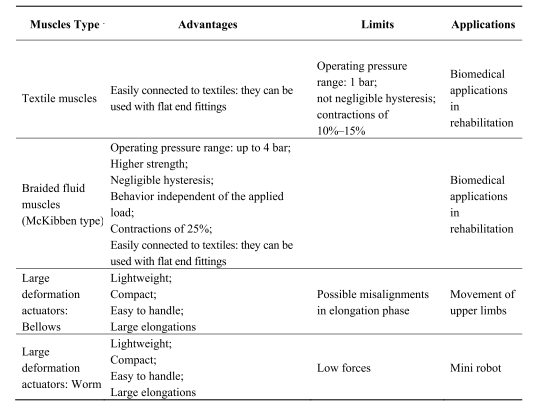
\includegraphics[width=1\textwidth]{Table_PAM_Features.png}
\end{table}

The first works on assistance to human lower limbs using soft robotics are in \cite{park2011bio,Hamedi2015}, which describes a soft orthosis for the foot intended to treat gait pathologies, particularly the drop-foot condition. One important aspect of this device is its design, inspired in the musculoskeletal human system, i.e. the actuation system was designed to comply a muscle-tendon-ligament functionality mimicking the natural behaviour of the human body (\autoref{fig:bio_ankle}). The soft orthoses is powered by pneumatic actuators, also called Mckibben-type actuators. They are attached to a soft support structure consisting of an adapted neoprene knee sleeve and a five toed leather shoe. A total of three off-the-shelf pneumatic muscles \autoref{fig:bio_ankle_parts}(a) assisted the dorsiflexion, eversion and inversion movements of the ankle joint by generating tension forces in artificial tendons, made of a flexible but non-extensible metal cable, positioned close to the foot tendons. The tendons were located inside a low friction material tube to prevent generated force losses; two of them were anchored to a single point in the foot brace while the other one was anchored in four different points in order to distribute the pulling force, again, mimicking the human body behaviour. The artificial ligaments provided with the same functionality as the biological ones, which is to restrict the movement of the tendons in all the directions other than the one of actuation (\autoref{fig:bio_ankle_parts}(b)). The pneumatic actuators were strategically anchored in two points, at the bottom of the knee sleeve providing nonrestrictive motion of the knee, and at the foot brace.
\begin{figure}[hbtp!]
    \centering
    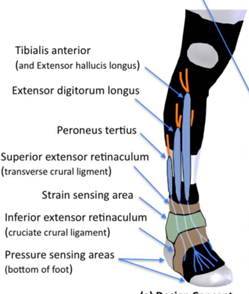
\includegraphics[width=0.4\textwidth]{BioinspiredAnkle.png}
    \caption{Design concept of the bio-inspired active soft orthosis for ankle foot. From top to bottom, the main parts are highlighted: artificial muscles attached to the soft wearable garment, a strain sensor for ankle angle measurements, the tendon-ligament system and pressure sensor for gait cycle detection \cite{park2011bio}. }
    \label{fig:bio_ankle}
\end{figure}
\begin{figure}[hbtp!]
    \centering
    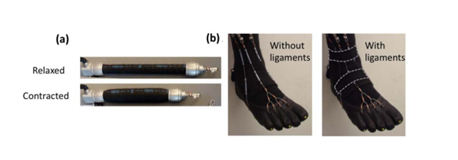
\includegraphics[width=\textwidth]{BioinspiredAnkleParts.png}
    \caption{Some components implemented in the soft orthosis, (a) pneumatic artificial muscle in its relaxed and contracted state and. (b) complete tendon-ligament system (right) and with-out ligaments (left). \cite{park2011bio}. }
    \label{fig:bio_ankle_parts}
\end{figure}

Another soft orthosis using pneumatic actuation is presented in \cite{Park2012} which extends the concept of embedded sensor and create an embedded sensor-actuator module, which is referred as a muscle-sensor unit. In order to obtain some degree of compliance with human's lower limb, the device has a cylindrical shape and it is made of a flexible silicone elastomer (EcoFlex 0300). The muscle-sensor units are embedded into the latter shape to form a distributed array of four columns and four rows (16 actuators), allowing the device to has plenty different motions and delivered torques depending on the number of activated actuators at a given time (\autoref{fig:soft_sleeve}). During the casting process, each column of actuators is tied to each other with Kevlar fibres so they can pull each other when contracting, also the fibres are anchored to both caps of the cylinder in order to achieve the desired movement. When the pneumatic muscle is activated its radius increase and its length decrease, creating a compression force. This design provides some degree of modularity due to the many embedded actuators which can be activated independently. Nevertheless, it has little compliance with the human's lower limb which ultimately complicates the conversion of generated forces into useful torques for assisting the joint of interest.
\begin{figure}[hbtp!]
    \centering
    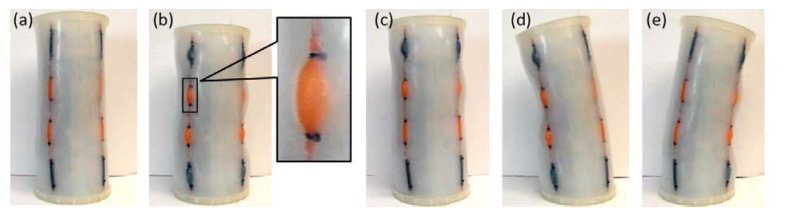
\includegraphics[width=\textwidth]{SoftSleeve.png}
    \caption{Different shapes achieved by the prototype. (a) Original shape. (b) All muscles activated, contracting the whole body and amplified image of one muscle. (c) Partial contraction, only the 1st and 2nd top rows are activated. Both (d) and (e) illustrates bending movements, only two adjacent columns are activated. \cite{Park2012}. }
    \label{fig:soft_sleeve}
\end{figure}

On the other hand, a novel implementation called virtual anchor technique, which used pneumatic artificial muscles, can be seen in \cite{wehner2013lightweight}. Addressing the challenge of force transmission using soft materials attached or strapped to the skin, which for high forces (such as the required in normal walking) results intolerable for the user, the key anchor points of the human body are defined as the ones exhibiting large bony landmarks. These regions are able to withstand high forces and minimize the slippage or chaffing of soft materials positioning on them. Furthermore, the virtual anchor technique was also motivated by the changes in length of some parts of the skin surface during joint motion in where some parts exhibit more changes than others. Therefore, the soft exosuit was developed by interconnecting PMAs and nylon straps, replicating the extensible and non-extensible paths of the skin, respectively, in the specific points where the changes in the skin length take place, also called virtual anchor points which in combination with the key anchor points allow a good transmission of forces without causing discomfort to the user. In \autoref{fig:anchor_concept} it can be appreciated the described concept, the orange lines represent the pneumatic actuators interconnected with the key anchors and the virtual anchors. The latter constrain the actuator's movements other than the desired, as well as redirect the actuator's reaction forces to the body areas able to sustain them. Finally, this design was able to reduce the metabolic cost caused by wearing the complete device of about 10 kg, by almost 100\%. Considering that no control system, other than a timed activation sequence, and no perception system was implemented, this technique opens the door for further improvements to achieve a better degree of assistance.

\begin{figure}[hbtp!]
    \centering
    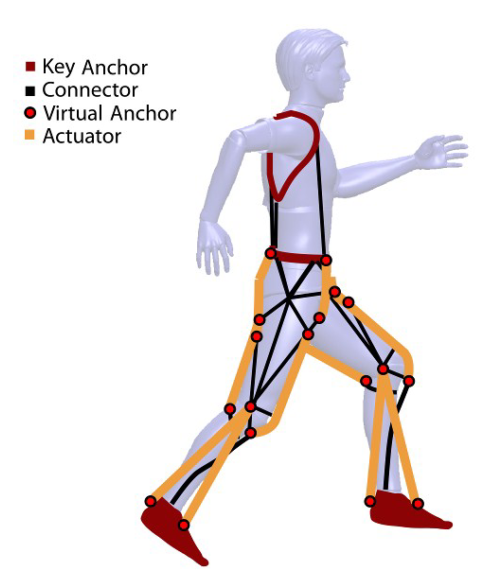
\includegraphics[width=0.45\textwidth]{AnchorConcept.png}
    \caption{Virtual anchor concept. The three key anchors (red square) located at the foot, hip and shoulder are interconnected with the soft actuators (orange) and auxiliary connectors (black) in specific points called virtual anchors (red circle) to stabilize the forces created by the actuators. \cite{wehner2013lightweight}. }
    \label{fig:anchor_concept}
\end{figure}

Putting aside the McKibben-type actuators as the most common choice for pneumatic muscles, elastomers such as high-flexible silicone can be used to build PAM as shown in \cite{Park2014}. This PAM consist of interconnected flat chambers made of silicone rubber which inflate when pressurized air is injected (\autoref{fig:Flat_elastomer}), the innovative concept in this work is the zero-volume air chamber which provides with a higher degree of compliance and compactness (traditional PMAs retain air inside them even when they are not actuated). Kevlar fibres are embedded inside this soft actuator to constrain the expansion direction and create a contraction movement when pressurized. The flatness of this actuators simplifies the casting process. Furthermore, the chamber based design make it possible to join each chamber together not only in series, which increases the contraction length, but in parallel as well to increase the contraction force. In order to test the actuator performance, a soft exosuit similar to the previously described was developed using nylon straps and hooks to connect the soft actuator to the points of interest. The developed soft orthosis, intended for infant-toddler rehabilitation, was able to deliver a 38 N contraction force and 18 mm contraction length by implementing a muscle with an array of four elastomer actuators inter-connected in series. In addition to, a total excursion for the knee joint of 132\textdegree{} was achieved, considering both flexion and extension motions (\autoref{fig:Flat_elastomer}). Moreover, in a most recent development by \cite{Low2016}, it can be found the implementation of elastomers for ankle assistance, in this case the pulling force of the PAM is generated when the actuator deflates and a pushing force is generated when it inflates, an inverted behaviour in comparison to previously mentioned applications. This soft orthosis consists of a regular sock which has attached to both ends the PAM, that is enclosed into textile to restrict its longitudinal and radial expansion mainly. Despite the simplicity and assistance capabilities of the device, it can't be worn with shoes, restricting the assistance to indoor activities
\begin{figure}[hbtp!]
    \centering
    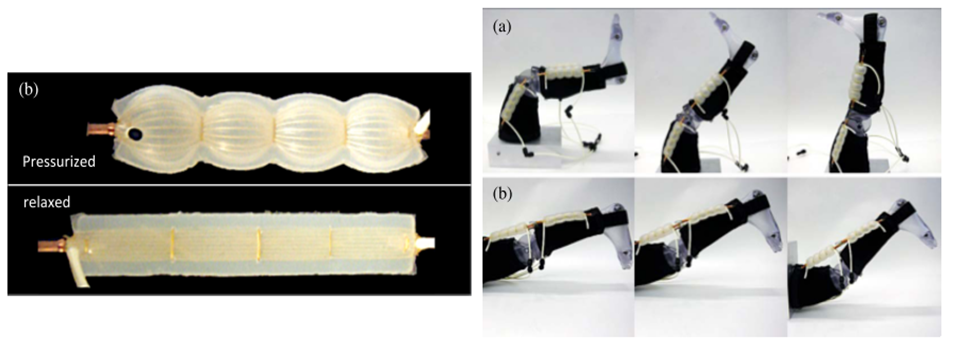
\includegraphics[width=1\textwidth]{FlatElastomer.png}
    \caption{Left: flat elastomer pneumatic actuator in its both relaxed and pressurized states. Right: illustration of the implementation of the flat actuator in medical leg model assistance, along with the achieved extension (a) and flexion (b) motion. \cite{Park2014} }
    \label{fig:Flat_elastomer}
\end{figure}

This concept of expanding, instead of contracting, the PAM when pressurizing is called Inverse PAM (IPAM). This very recent type soft actuator, called `Hydro Muscle', is directly compared with McKibben muscles since it overcomes the main limitations of the latter. The main difference between this actuator and the previously mentioned is the shift from pneumatic technology to hydraulics, in fact, it is reported that the pressure found in homes tap water is enough to actuate it \cite{Sridar2016}. Therefore, the cylindrical shape `Hydro Muscle' is capable of elongating axially, increasing its stiffness radially, when pressurized; and of the exact opposite behaviour when depressurized (\autoref{fig:IPAM}). The actuator functionality is due to two structural layers of different materials. The inner layer is a tube made of an elastic material (latex showed better performance than the commonly used silicon) and the outer layer is made of a soft but inelastic material, such as polyester, which restricts the inner layer radial expansion and allows its axial expansion. Despite the simplicity of the design, this new concept of actuator is free of energy losses in radial expansion. Also, the energy losses inherent when using compressed air as the power source are not presente in this design (in comparison to PAMs).
\begin{figure}[hbtp!]
    \centering
    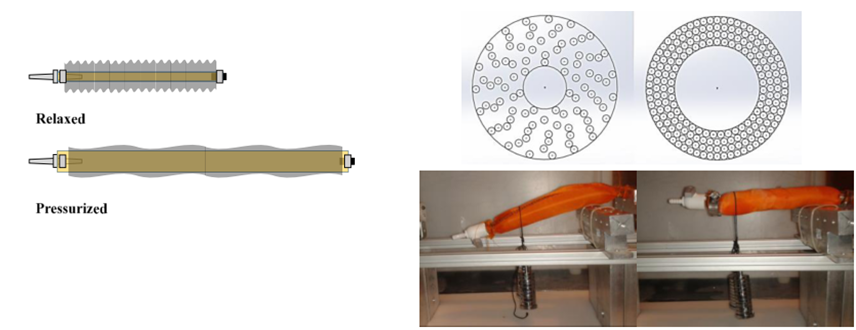
\includegraphics[width=\textwidth]{IPAM.png}
    \caption{Left: Illustration IPAM developed in its relaxed and pressurized state, the small radial expansion and large axial expansion is appreciated. Right: Cross-sectional view of the jamming effect ongoing inside the actuator (top), and bending effect (bottom) caused by heavy load, left hand side image, and correction of the bending using the jamming effect, right hand side image. \cite{Sridar2016}. }
    \label{fig:IPAM}
\end{figure}

The experiments performed in the paper showed that this innovative soft actuator is 33\% more efficient in comparison to a McKibben muscle using hydraulics. Furthermore, this actuator can be easily manufactured with off-the-shelf components. On the other hand, the convenience of using both pneumatic and hydraulic muscles for performing pulling instead of pushing tasks, is to prevent the bending effect caused when the actuator is fixed in one of its ends and has a heavy load attached to the other end. The latter effect is amplified for pushing tasks being one of the main drawbacks of the proposed actuator concept. However, a pr-posed solution is to use the principle of jamming by filling the gap between the inner and out-er layer with granular media which will jam when the actuator is pressurized (\autoref{fig:IPAM}). Another IPAM development can be found in \cite{Hawkes2016} which implemented a very similar concept as the previously mentioned, however, this IPAM managed to achieve a strain of 300\% the length of the developed actuator whilst the previously mentioned IPAM only achieved a 100\% strain. The improvement in the achievable strain was mainly to the complete restriction of the stretchable material in the inner layer to only expand along its axis and not radially. Furthermore, the main benefits of IPAM in comparison with PAM are reported as follows: high strain and nearly linear control (since no radial deformation is present). The ability to achieve high strains make these soft actuators suitable for joints like the elbow.

\subsubsection{Cable-driven Actuators} \label{sec:cable-driven}

Another actuation technology implemented in soft orthoses are the Bowden cables in combination with electrical motors. Following the same principle as pneumatic muscles, this technology relies on generating tensions along a cable which, with a right positioning along the human lower limb, can transmit torques to the human body. The work in \cite{asbeck2013biologically} presents the design and implementation of a battery operated soft exosuit built with Bowden cables (\autoref{fig:bowden_exo}), which is battery operated. 
\begin{figure}[hbtp!]
    \centering
    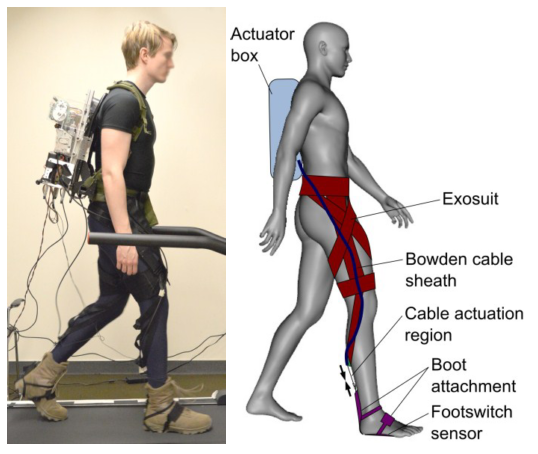
\includegraphics[width=0.5\textwidth]{BowdenExosuit.png}
    \caption{Developed Bowden cable-based soft exosuit prototype (left). Illustration of the initial design concept highlighting the main parts of the soft exosuit. \cite{asbeck2013biologically}. }
    \label{fig:bowden_exo}
\end{figure}

The exosuit is based on the leg's muscles functionality during normal walking, with the objective of assisting the forward propulsion stage of the gait. The soft exosuit structure made of fabrics is attached to the waist and above the knee, from the former the Bowden cable follows a path of webbing straps into the lower limb, ending at the ankle. In order to minimize the webbing strap structure chaffing and displacement when tensions are created along it, the strap along the waist of the user terminates at the hip since it is a bony part, i.e. there is almost no muscle and fat tissue between the skin and the bone, ultimately improving the exosuit stiffness. On the other hand, the suit delivers 18\% and 30\% of the torques required for normal walking on the knee and hip, respectively. However, despite the innovative design, the exosuit structure have limitations on the degree of compliance and stiffness, resulting in an approximately 13 cm displacement of the exosuit, when the Bowden cable is actuated. The biggest reported limitation during the experiment was the inefficiency of the Bowden cables, almost 45\% of the mechanical power generated by the actuator is lost, mainly in friction. However, the implemented multi-joint concept allows the actuation of two joints using a single actuator.

Following the multi-joint actuation concept, another soft exosuit is designed in \cite{Bartenbach2015} with the objective of not only provide assistance but to enable impaired users. The concept (\autoref{fig:bowden_exo2}) exploits the benefits of using a single Bowden cable actuator to control more than one joint, multi-joint actuation. The difference in this case is the deep analysis performed regarding the compatibility of the joints, taking into account synergy of torque and equal polarity of torque, as well. In order to assist the desired movements of sit-to-stand, walking and stairs ascend, the knee and the hip joint were selected as the most suit-able combination. Despite the fact the work was limited to describe the concept and design, by analyzing the selected joint combination it is expected to support the movements of sit-to-stand and stairs ascend.
\begin{figure}[hbtp!]
    \centering
    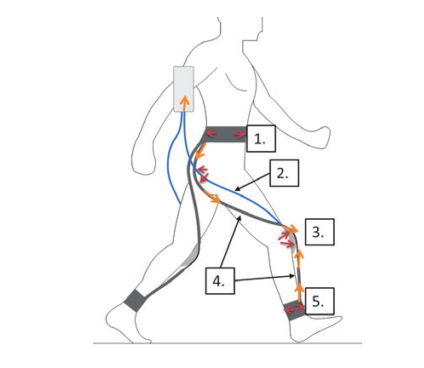
\includegraphics[width=0.7\textwidth]{BowdenExosuit2.png}
    \caption{Soft exosuit implementing the multi-joint actuation concept. A Bowden cable actuates the suit (2) by contracting the webbing element anchored at the hip (1) and shank (5). Reaction forces and actuation forces are represented in red and orange arrows respectively. \cite{Bartenbach2015}. }
    \label{fig:bowden_exo2}
\end{figure}

The next follow up on the concept of multi-joint actuation is documented in \cite{Ding2014} where a testing platform for soft exosuits was developed. The aim of this platform is to study the performance of the multi-joint actuation concept when being implemented in different soft exosuits. The off-board platform integrates the Bowden cable actuators and the sensors required to evaluate their performance. In addition to, this platform can deploy sensors to be attached to the exosuit and compare relevant metrics such as mechanical power efficiency. This platform, which can be re-configurable to meet different applications, has been used to evaluate the advantages of implementing single joint and multi-joint actuation \cite{Ding2016}, highlighting the benefits of the latter. Furthermore, the study performed with the aid of this platform provided with designing parameters for the development of an exosuit, in other words, the multi-joint platform assists the designing phase, ultimately reducing designing times.

\subsubsection{Shape Memory Materials}

The main two groups of shape memory materials implemented in soft robotics are: shape memory alloys (SMA) and shape memory polymers (SMP). Both technologies function under the same principle: they are able to switch into a different shape when a stimulus such as heat is in contact with them. Nevertheless, there are some differences to be mention. The SMA have to main phases, one for high temperature (austenite) and one for low temperature (martensite), when they suffer deformation while being in the martensite phase they can recover from the deformation by exposing them to heat, therefore SMA convert the energy from heat into mechanical energy to return to their original shape \cite{ImagesScientificInstrument2016}. This property is usually exploited to cause contraction changes in the mate-rial (\autoref{fig:SMA}). Therefore, SMA are commonly used in tendon-driven applications.
\begin{figure}[hbtp!]
    \centering
    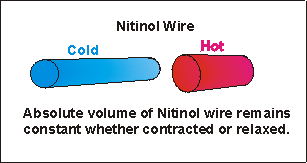
\includegraphics[width=0.5\textwidth]{SMA.png}
    \caption{Shape memory alloys made of Nitinol. The contraction effect under the increase in temperature is illustrated \cite{ImagesScientificInstrument2016} }
    \label{fig:SMA}
\end{figure}

The implementation of SMA into robotic applications have three main challenges to be addressed: response speed, high power consumption and low operational bandwidth. SMA make use of the Joule effect present in metals when an electric current flows through it, which generates heat. Depending on the metals used in the alloy, the amount of heat required for the SMA to recover from deformation is high enough to melt plastics, this excess of energy is what make SMA inefficient \cite{Bundhoo2009a}. Furthermore, the large time required to cool down the SMA in order to repeat a cycle of deformation-recovery is another limitation which limits the operation frequency. This cooling process is usually performed by air convection which explains the large time (several seconds) required \cite{Bundhoo2009}. Therefore, SMA have been found to be unsuitable for orthoses or prostheses. However, plenty of authors have successfully develop the latter devices, in both rigid \cite{tarkesh2007} and soft variations \cite{Stirling2011}, capable of assisting human motions proving to be suitable for applications such as clinical rehabilitation where slows and repetitive cycles are required \cite{Pittaccio2009,Chenal2014}. Two comprehensive reviews documented in \cite{pittaccio2012shape} and \cite{Coral2012} illustrates the many other applications where SMAs are being implemented in the field of rehabilitation, such as: re-positioning, muscle toning, functional exercise and assistive robotics. Moreover, the review done by W. Coral also describe many works focused on addressing the SMA limitations.

The very interesting work done by J. Zhang in \cite{Zhang2013a} describes a SMA-based artificial muscle. This configuration facilitates the addition of a cooling system, due to the cylindrical hollow shape of the artificial muscle. Therefore, a mini pump is used to create a flow of air inside the artificial muscle which is able to reduce the cooling time by 10 times. The performance of this artificial muscle is further improved by taking into ac-count the hysteresis behaviour typically found in SMA when shifting between the low and high temperature phases. Furthermore, there is again evidence of trying to replicate the muscle-tendon functionality, in this case by adding a spring in series with the artificial muscle which aids the SMA recovery phase and simulate a more realistic condition to the one at which the human muscles are subjected. The author is the first one able to model this behaviour and develop an adequate controller, which can be implemented in other scenarios involving SMA. Finally, this artificial muscle is implemented into an active foot orthosis (\autoref{fig:SMA_orthosis}) which achieve large contractile forces by using in parallel more than one SMA wire to form each of the pulling tendons. The main drawbacks were having low efficiency and low operational bandwidth.

\begin{figure}[hbtp!]
    \centering
    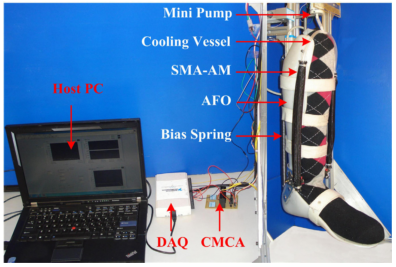
\includegraphics[width=0.7\textwidth]{SMAOrthosis.png}
    \caption{Illustration of the developed soft orthosis for the ankle joint. The developed SMA artificial muscle along the main parts are highlighted. \cite{Zhang2013a}. }
    \label{fig:SMA_orthosis}
\end{figure}

Many attempts to improve SMA bandwidth have been made and since the theoretical bandwidth for a SMA is 3\% of its length, the most obvious approach is to increment the length of the SMA wire for a particular actuator but without increasing the length of the actual actuators. The latter can be achieved by using pulleys on each end-point of the actuator to develop, which allows the SMA wire to effectively increase its length without increasing the actuator length. However, implementing solely pulleys in a soft actuator greatly reduce compliance, increase the actuator weight and may cause twisting between the individual turns of the SMA wire. Therefore, a new approach described in \cite{Villoslada2015} propose the implementation of Bowden cables outer sheath to contain the SMA wires inside. This concept allows the SMA to be directed in many ways to the point of interest, allowing the actuator to have different shape that can be compliant with the user's body, e.g. the SMA can be wrapped around the user's arm in a solenoid-like shape which also increase the SMA wire length (\autoref{fig:flexible_actuator}). Furthermore, pulleys are also implemented to allow the SMA to have a maximum number of three turns contained inside the Bowden sheath. Two main drawbacks were discovered during an experimental testing: SMA wires were twisting between each other which caused high friction losses and prevented the SMA to recover its initial length completely; the other drawback was the Bowden sheath material which was found to have low force transmission efficiency. In order to solve the latter, the Bowden cable sheath made of nylon was replaced by flexible tubes of Polytetrafluoroethylene (PTFE) and every SMA wire turn was individually encased in a narrow-gauge sheath. The final experiments showed that the developed actuator is able to contract 9\% of its length which is three times the theoretical contraction length of an SMA wire.

\begin{figure}[hbtp!]
    \centering
    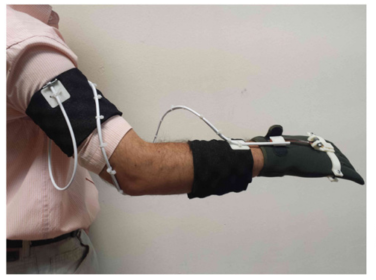
\includegraphics[width=0.5\textwidth]{FlexibleActuator.png}
    \caption{Flexible actuator around the arm in a wrist exoskeleton prototype. \cite{Villoslada2015}. }
    \label{fig:flexible_actuator}
\end{figure}

Shape memory polymers are a little bit more complex than SMA. They have two main phases: a glassy state (high stiffness) and a rubbery state (low stiffness). Furthermore, when they are in their rubbery state, they can be deformed by applying small forces and preserve the deformation by cooling the SMP. In this state, the SMP can be considered rigid and it has to be heated to the point of the transition temperature to return to its original shape, hence having shape memory. This property of preserving a deformation is analyzed by K. Takashima et al. in \cite{Takashima2010} in an attempt to boost the McKibben artificial muscle performance. McKibben actuators are unable to maintain their contraction shape un-less precise and continuous control is implemented which cause premature wear on controlling elements as well as increase energy consumption. Therefore, a SMP is embedded into the McKibben braid which, by controlling the SMP temperature, allows the artificial muscle to hold its contracted position as illustrated in \autoref{fig:mckibben}. It is worth mentioning that SMP can be stimulating in different ways to obtain the change of shape, such as infrared light, electric field, magnetic field and even manipulating the material water content. In this work, the SMP made use of a heating source as well as compressor which drastically limited the developed actuator portability, but as previously mentioned, different stimulus sources can be used for different SMP.

The positive factors when comparing a SMA with a SMP are described, being the SMP benefits: light weight, low cost, rigidity in low temperature and flexibility in high temperature, higher strains, hence length deformation (around 400\% in comparison with 7\% for SMAs) and 3D shapes can be easily created. Furthermore, the main positive aspects of the improved McKibben are: allows rigidity fixing, the parameter to control stiffness can be used to control actuation and controllability of the actuator surface by individually stimulating certain segments of the SMP.

\begin{figure}[hbtp!]
    \centering
    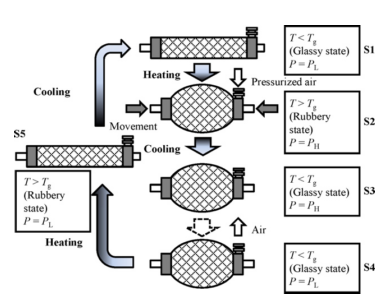
\includegraphics[width=0.8\textwidth]{Mckibben.png}
    \caption{Schematic illustrating McKibben with embedded SMP functionality \cite{Takashima2010}. $T_g$: transition temperature, $P_H$: high pressure, $P_L$: low pressure. }
    \label{fig:mckibben}
\end{figure}

\section{Soft Perception Technologies}
\subsection{Liquid metal alloys embedded into elastomers}

Strain soft sensors made of liquid metal alloys embedded into soft materials are being implemented into soft orthoses, such as the one in \cite{park2011bio}. The materials used in this case were Eutectic Gallium Indium (eGaIn), as the liquid metal alloy and flexible silicon rubber layer, which creates a really flexible sensor, \autoref{fig:strain_sensor}. The sensor was implemented to measure changes in the ankle joint proportional to the skin strain which it was attached to, by measuring the changes in resistance caused by the variations in the path length and cross-sectional area of the channel containing the liquid metal. Nevertheless, the developed soft orthosis implemented two other non-soft sensors: an inertial measurement unit (IMU) as an angle position detection and a pressure sensor attached to the shoe insole to detect foot strikes, hence the gait cycle. The developed strain sensor delivered good performance and contributed in the developed of a feedback controller for this soft orthosis.

\begin{figure}[hbtp!]
    \centering
    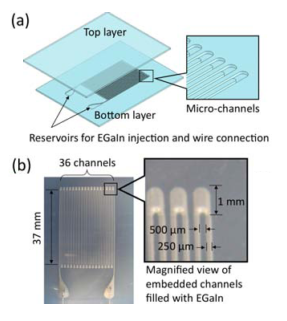
\includegraphics[width=0.4\textwidth]{StrainSensor.png}
    \caption{Illustration of a soft strain sensor. The microchannel filled with liquid metal can be appreciated in the prototype (b) and concept design (a). \cite{park2011bio}. }
    \label{fig:strain_sensor}
\end{figure}

Liquid metal alloys are also implemented in \cite{Park2012}, as previously described, in the form of embedded muscle-sensor units (\autoref{fig:soft_sleeve_sensor}). The soft strain sensor was able to estimate the contraction length of a pneumatic muscle by measuring its radial expansion. In order to preserve softness, thin flexible copper wires were embedded into the cylindrical soft orthosis to obtain the sensor readings.

\begin{figure}[hbtp!]
    \centering
    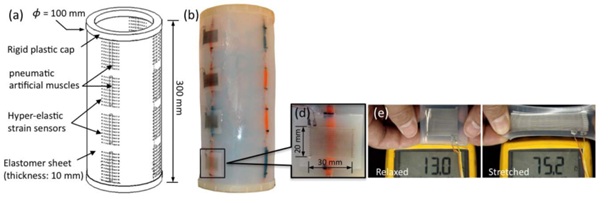
\includegraphics[width=0.8\textwidth]{SoftSleeveSensor.png}
    \caption{(a) Design concept. (b) Developed prototype. (d) Magnified view of the embedded sensor-actuator concept. (e) Soft strain sensor change in resistance during stretch. \cite{Park2012}. }
    \label{fig:soft_sleeve_sensor}
\end{figure}

Taking a step further the application of soft strain sensors with eGaIn, in \cite{mengucc2013soft} is presented a wearable soft suit capable of sensing the joint angles of the hip, knee and ankle joints (\autoref{fig:Sensing_suit}). With the sensors properly positioned along the lower limb, by measuring the strain caused by the joint rotation it can be known the joint angle. The sensors were able to track motions with a mean absolute error of 8\textdegree{}, being the most precise tracking achieved on the hip joint and the less precise on the ankle joint. In the mentioned work, only sagital plane motions were measured, however, due to the great success and linearity of the sensors, they are planned to be implemented to measure motions in the frontal plane as well. The complete suit characterization can be found in \cite{mengucc2014wearable}.

\begin{figure}[hbtp!]
    \centering
    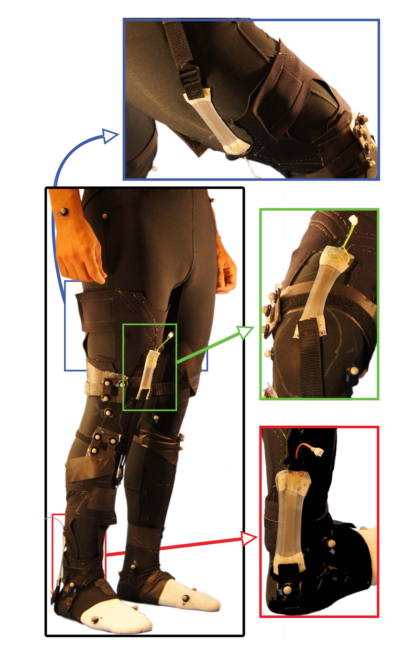
\includegraphics[width=0.4\textwidth]{SensingSuit.png}
    \caption{Implementation of soft strain sensors into a Soft sensing suit, from top to bottom: hip sensor, knee sensor and ankle sensor position. \cite{mengucc2013soft}. }
    \label{fig:Sensing_suit}
\end{figure}

On the other hand, a potentially improved version of these soft strain sensors is presented in \cite{Chossat2013} where the highly stretchable elastomer is filled with two different conductive liquids, a traditional liquid metal and an ionic solution, instead of one. Interconnecting the strain soft sensor with the external application has been a big challenge, since the strain caused by the connection, usually soft wires, affects the sensor accuracy by increasing the total electrical resistance and by generating additional strain. Nevertheless, the ionic solution is intended to decouple the signal routing part from the sensing part in order to solve the latter challenge, creating a noise-free interface with the external application (\autoref{fig:hybrid_strain_sensor}).

\begin{figure}[hbtp!]
    \centering
    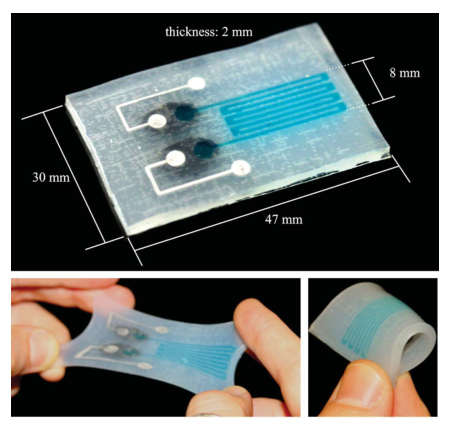
\includegraphics[width=0.5\textwidth]{HybridStrainSensor.png}
    \caption{Hybrid soft strain sensor, the interface between the liquid metal and the ionic solution can be clearly seen in dark areas. \cite{Chossat2013}. }
    \label{fig:hybrid_strain_sensor}
\end{figure}

One direct implementation of the embedded microchannel with conductive fluid sensors, can be seen in a recent improvement to the McKibben type PAM \autoref{fig:braided_sensor}. McKibben actuators were strongly adopted in soft robotics applications and there is plenty of information in the literature about their implementations, modelling, etc. However, accurately sensing these actuators parameters such as deformation and force when they are pressurized was still a challenge being addressed in many forms such as: cylindrical dielectric elastomers with carbon grease disposed on their surface to function as electrodes \cite{Goulbourne2007}; and attaching to the actuator an elastomer sheath with microchannels filled with conductive fluid which surround the actuator in a helical shape \cite{Park2013}. Both the microchannels and the electrodes represent a resistor which will change its physical dimensions, by extension its electrical resistance, when the actuator com-press or stretch which provides a measure of the actuator deformation. Furthermore, the idea of a helical path surrounding the actuator was extended to a solenoid shape and to the so called 16 helices shape, as shown in \cite{Felt2014,Felt2015}. From the electric circuit created is possible to measure both the output force and length deformation of the actuator by correlating them with the circuit resistance and inductance respectively. This work proposed the implementation of conductive wires to build the reinforced braid of a McKibben actuator allowing the actuator to `sense', from there the given name of `Smart Braid', creating a solenoid like circuit from which the inductance can be measured using a couple of mathematical approximations such as: the Neumann approximation (for the 16 helices shapes) and the long solenoid approximation, being the former one the most accurate and general; but at the same time the most expensive in terms of computation. The author exerts that this new sensing concept can be applied to multitude of scenarios in soft robotics, which includes soft orthosis.

\begin{figure}[hbtp!]
    \centering
    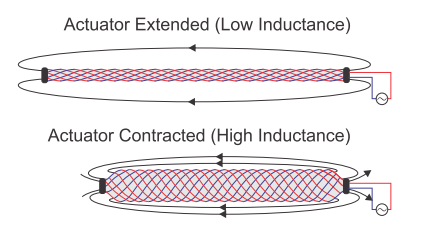
\includegraphics[width=0.5\textwidth]{BraidedSensor.png}
    \caption{Illustration of the `Smart Braid' concept. The variation in the actuator length cause a change in the electric circuit inductance. \cite{Felt2015}. }
    \label{fig:braided_sensor}
\end{figure}

\section{Control Technologies} \label{sec:controlSystems}

One of the successfully implemented control systems is documented in \cite{park2011bio}, which is the ankle soft orthosis previously mentioned. The control system is comprised of several micro-controllers for parallel processing, and is divided into four main stages: sensing, signal processing, control and actuation (\autoref{fig:control_system}). The soft orthosis makes use of three different sensor technologies which requires different sampling and signal processing algorithms for each one, being the IMU the most complex one. Thereafter, another micro-controller with access to all the sensor, makes the decision to activate the solenoid valves that controls the pneumatic muscles by generating a pulse width modulating (PWM) signals which in combination with binary on/off valves are able to perform a proportional control type. No mathematical model was deducted to describe the non-linear behaviour of the pneumatic muscles, instead, simpler controller approach as forward feedback and feedback controller were implementing, with the latter being able to achieve a response time of 500 ms when a perturbation was present on the system, as letting hang a weight from the device toe. The feedback controller made use of a soft strain sensor (previously mentioned) to correct the ankle angle. Finally, although the controller performance is good it is still not enough to provide active gait assistance nor to predict user intentions. Another drawback, minor in this case, is that the system requires for calibration every time a new user wears it. Nevertheless, the developed soft orthosis is suitable for rehabilitation because it can achieve a dorsiflexion of 12\textdegree{} and 20\textdegree{} when foot was at resting position, and when foot was forced to a plantarflexion position, respectively; in addition to, the perception system could provide the clinician with meaningful data about the patient progress. The previous work was continued in \cite{park2014design} where a new controller was designed by considering the interaction between the soft exosuit and the human body as a black box, i.e. instead of trying to model the non-linear behaviour of the whole system some experiments were performed to obtain a system input/output relation-ship and after that implement classic control techniques to model a linear time invariant controller. The results were promising since the original complex system was able to perform accurately using simple techniques. Finally, the addition of electromyography sensors was dis-cussed to add the involuntary muscle contractions of the user into the system as a disturbance and improve the accuracy during different scenarios.

\begin{figure}[hbtp!]
    \centering
    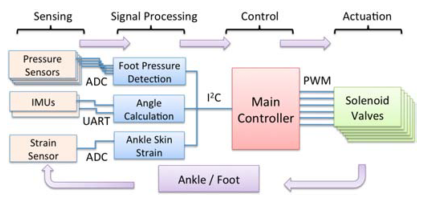
\includegraphics[width=0.7\textwidth]{ControlSystem.png}
    \caption{Control system architecture implemented for the ankle soft orthosis. \cite{park2011bio}. }
    \label{fig:control_system}
\end{figure}

In some cases, the design and development complexity of a controller for soft devices restrain the research extend to focus only in the implementation and study of soft actuation and perception systems. This is the case in \cite{Park2012}, the cylindrical soft sleeve with embedded muscle-sensor units; where the developed controller is well designed but with no close-loop architecture nor complex mathematical model to predict the soft material behaviour. Again, the controller system is integrated by several micro-controller units, each of those communicated with their surroundings neighbours, in fact, each of the 16 nodes embedded into the cylindrical soft sleeve has one. Furthermore, each controller architecture has two layers, one dedicated to the collection of sensor data, intercommunication between the micro-controller units, specify actuation parameters and schedule of tasks. The scheduler is implemented as a mean to synchronize the otherwise independents micro-controller units and behave as a network, converting the system into a sequential one instead of a parallel one as the previously mentioned. Every unit has four tasks to execute at a given time and a given order: sensing, communicate, process data and actuate. On the other hand, the actuation parameters are generated using a mathematical approximation of the soft material behaviour which assumes no deformation is caused by the compression of the pneumatic actuators, other than the length change present where the actuators are embedded, this means the diameter of the cylinder d remains constant as well as the length l in the other side of the cylinder. The experiment proved the requirement of a better approximation, since for a desired bending angle of 15\textdegree{}, an actual bending of 11.5\textdegree{} was achieved, and feeding the soft sensors data into the mathematical approximation, a bending of 13\textdegree{} was estimated; therefore, achieving an accuracy of 76\%.

The fact that few soft exosuit developments fully implement a controller system does not imply that no research is being performed in the field. The implementation of current soft actuators into functional devices, as well as the proof of concept of emerging soft actuators are usually followed by an extensive study about modelling their behaviour to translate that information into a controller system. Solely for PMAs several work has been done, even implementing fuzzy logic to achieve better results, in \cite{Chang2015,Skorina2015,Bishop-Moser2015,Hosovsky2016}. The next step in the research cycle of all the soft actuation technologies is to implement the tested models into functional devices, which then will allow new concepts to be developed, hence new modelling research to be performed.

\section{Gaps in the Body of Knowledge} \label{sec:gaps}

The available literature suggest a growing interest in the research and development of soft actuation technologies, soft perception systems, and control systems to pair with the latter two. Also, and following the bioinspiration driving the field of Soft Robotics, many works are attempting to imitate the capabilities of the human musculoskeletal system by developing soft actuator that behave like the human muscle-tendon component. This is more evident when looking at the available works on Pneumatic Artificial Muscles (PAMs) described in \autoref{sec:PMAs}, where an actuator is used as the contractile force generator element (muscle), and a flexible interface (tendon) is used to transmit that force to the desired location. Similarly, established technologies such a electric motors, which are able to deliver forces in both direction of rotation, are being used in combination with Bowden cable to create pulling forces, as mentioned in \autoref{sec:cable-driven}. This type of setup is known as a redundant system because more than one actuator is required to control both directions of rotation of a joint. Moreover, the research and development of new soft materials, such as the SMA and SMP, is also focused on creating materials able to contract when stimulated. There is still plenty of work to be done in this matter, which is why this is identified as one gap in the body of knowledge.

The vast majority of available literature is focused on testing a new soft actuation concept in an open-loop approach, i.e. with no control system implemented. This is caused by the fact that modelling the mechanical behaviour of a soft material is very complex. Even the control system of the most documented work in the literature, the ankle-foot orthosis, does not implement a modelling technique to monitor the behaviour of the PMAs, instead it is focused on extracting as many information as possible from the environment and use this to decide when and how to activate the PMA \cite{park2011bio}. The scarce literature about the control systems of soft robotic applications, as evidenced in \autoref{sec:controlSystems} is identified as another gap in the body of knowledge.

Therefore, we have detected two main gaps in the body of knowledge which are addressed by this research. On the one hand, there is still many work to do in understanding the functionality of the human musculoskeletal system, and in developing a soft actuation technology which mimics the functionality of the muscle-tendon component. On the other hand, there is a lack of reliable modelling tools to predict the complex mechanical behaviour of soft materials being used in soft actuation technologies. 

\section{Summary}

According to the literature, the most commonly implemented soft actuation technologies in soft robotic applications for human assistance are: Pneumatic/hydraulic artificial muscles, cable-driven actuators based on electric motors, and shape memory alloys/polymers.  In cable-driven actuators, the amount of generated assistance is proportional to the electric motor mechanical output power. This means, large forces can be generated to even enhance the user capabilities, yet again, the transmission of this forces via the human body prevents this enhancement. A common problem is the relative displacement of the soft structure worn by the user when tensile forces are generated by the pulling action of Bowden cables. Nevertheless, one advantage of this technology in soft exosuits is the `remote' actuation capability, which means that the electrical motors can be placed distal to the joint to be assisted, concentrating the weight of the heavy parts of the soft exosuit in convenient locations of the human body, e.g. as a backpack. Another advantage of this technology is the flexibility of the Bowden cables which allow them to be deployed in many different trajectories along the human body, facilitating the use of the body parts capable of sustaining high forces.

In contrast, the other two soft technologies are commonly placed proximal to the joint to be assisted, which might allow a better distribution of the soft orthosis weight. Recent works have tackled the main limitations of PAMs, SMA and SMP. Particularly, big improvements have been achieved for PAMs and SMA. For the case of PAMs, the traditional and extensively implemented McKibben type muscle have been improved in terms of performance by the development of the Inverse PAM (IPAM). This latter technology surpasses the McKibben type muscle in assistance capabilities, efficiency and controllability. Furthermore, the concept of the IPAM can be also implemented using hydraulics which again comes with several advantages, a crucial one, the amount of exerted force. The main disadvantage of both pneumatic and hydraulic actuators is the needs for a compressor unit, which greatly decrease the soft orthosis autonomy and portability. Nevertheless, the recently developed `Hydro Muscle', which use pressurized water from a home tab, greatly increases the appealing of this technology. In a similar way, the greater efficiency of IPAMs allows portable tanks with pressurized air to be used.

The situation is quite similar for SMAs, many of the limitations from this technology, such as  as low strain, slow speed response and complex controllability have been addressed and improved. However, this technology is still in its early stages and their main drawbacks, such as high energy consumption and being unsafe for human interactions applications due to the high levels of heat they reach, make them unsuitable to be deployed in real soft robotic applications.

In the field of soft sensors, one of the main advantages of the soft strain sensors is that they can be custom-built to fit any application. When characterizing these sensors, two parameters are always mentioned: the electrical resistance and the gauge factor, the latter relates the strain with the change in resistance. Despite they original purpose of measuring strain changes, they can be used for angle measurements. On the controller side, the amount of research being performed in modelling the complex behaviour of soft actuators is slowly but constantly increasing. Nevertheless, the complexity and time consuming of tackling the latter is evidenced in the scarce literature available.

In summary, this literature review highlighted a very specific and bioinspired trend in soft robotic applications for human assistance, which is mimicking the human musculoskeletal system, specifically the muscle-tendon component. This approach is very compatible with soft technologies that are commonly placed proximal to the assisted joint (PAMs, SMAs, IPAMs, etc.), and many soft artificial muscles have already been developed. These works, however, have mainly focused on the contractile element of the muscle-tendon component, leaving plenty of room to research about the viscoelastic element, the tendon. The most straightforward to study the potential benefits of mimicking the human tendon behaviour, is to incorporate soft materials, to current soft actuation technologies, as part of the mechanism to transmit the generated forces. Essentially, creating a soft artificial tendon. Nevertheless, the success of maturing the previous concept into a soft robotic application greatly depends on having a reliable modelling tool which predicts the mechanical behaviour of soft materials. Finally, as mentioned in \autoref{sec:gaps}, this research aims to address two main gaps in the body of knowledge. On the one hand, the lack of literature about the implementation of soft materials as part of the force transmitting mechanism, which could allow for a better mimicking of the human musculoskeletal system. On the other hand, the lack of a modelling tool able to predict the mechanical behaviour of soft materials.

\chapter{Mimicking of the Human Skeletal Muscle System}

\begin{center}
    \textit{Material in this chapter is partially based on:}\\
    Solis-Ortega, R.D., Dehghani-Sanij, A.A. and Martinez-Hernandez, U.\\
    Characterization of kinetic and kinematic parameters for wearable robotics.\\
    \textit{Proceedings of the Conference Towards Autonomous Robotic Systems:} 548-556, 2017. \cite{solis2017characterization}\\
\end{center}

\section{Introduction}

Previously, the bioinspired trend of mimicking the human skeletal muscle system, specifically the muscle-tendon component, in soft robotic for human assistance was identified. The available literature mainly focus on the muscle component. In line with the aims of this research, this chapter is focused on understanding the biomechanics of the human body, specifically of the lower limb due to the impact of this section of the body in the ADL. Therefore this chapter is divided as follows.
Section one focuses on understanding the terminology involved in the biomechanics of the human lower limb. In section two, many clinical trials, also known as gait analysis, are reviewed to characterize the parameters of torque, angle, and power of the human lower limb during ADL. Section three describes the muscle-tendon component from a mechanical perspective. Section four introduce many recent works and approaches which attempt to translate the functionality of the muscle-tendon component into soft robotic applications. Section five describes how recent works are addressing the lack of modelling tools for soft materials, considering two main modelling approaches: model-driven and data-driven. Finally, the last section presents a summary of the relevant findings of this chapter.

\section{Biomechanics of the Human Lower Limb}

The common terminology used in clinical trials for the lower limb make use of the three planes of action of the human body to name the motion of a given joint of the body. These three planes are called sagital, frontal and transverse (horizontal) \cite{PhysicalSolutions2016}. Along with the three planes come three axes used to identify specific motions: frontal horizontal axis, vertical axis and sagital horizontal axis. The positioning of each of them is illustrated in \Cref{fig:body_planes_axes}. The sagital plane divides the body vertically into left and right parts, the frontal plane divides the body vertically into front (posterior) and back (anterior) parts and the transverse plane divides the body horizontally into upper (superior) and lower (inferior) parts.

\begin{figure}[htbp!]
    \centering
    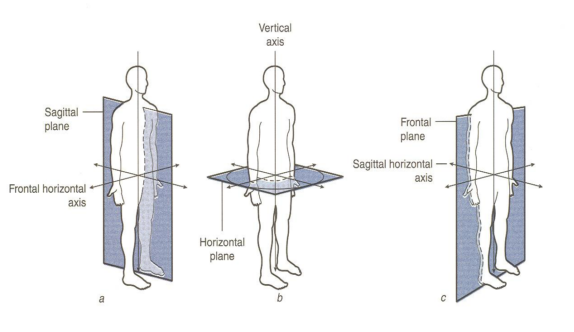
\includegraphics[width=\textwidth]{BoydPlanesAxes.png}
    \caption{Description of the three dimensional space used to understand human motions. \cite{PhysicalSolutions2016}. }
    \label{fig:body_planes_axes}
\end{figure}

Similarly, the motions of the human joints are named according to the plane and axis in which they are executed, which allows for easy recognition of certain motion (\Cref{fig:lower_motion}). There are ten different motions, grouped into five pairs, governing the lower limb of the body:
\begin{itemize}
    \item Flexion and extension describes the bending motion which shortens, or increase the angle between two parts of the body, respectively.
    \item Abduction and adduction describes the motion away from, or towards the body midline, respectively.
    \item Eversion and inversion of the foot describe the motion away from, or towards the body midline, respectively.
    \item External rotation and internal rotation describe the motion away from, or towards the body midline, respectively.
    \item Horizontal abduction and adduction describes the motions away from, or towards the body midline, respectively.
\end{itemize}

\begin{figure}[htbp!]
    \centering
    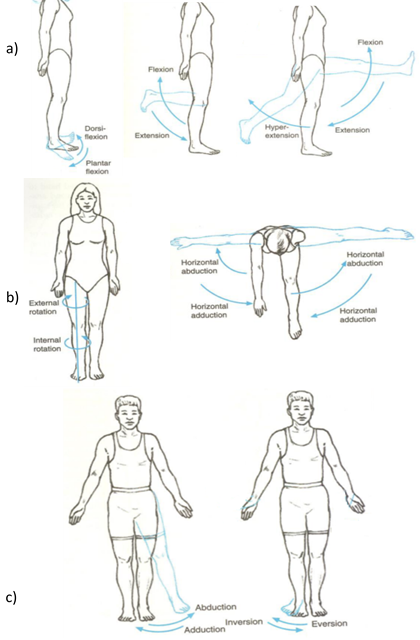
\includegraphics[width=0.8\textwidth]{LowerLimbMotionTerminology.png}
    \caption{Illustration of lower limb motions for a) sagital plane, b) frontal plane and c) transverse plane. Image adapted from  \cite{PhysicalSolutions2016}. }
    \label{fig:lower_motion}
\end{figure}

\section{Characterization of Kinematic and Kinetic Parameters for Activities of Daily Living}
\label{sec:characterizationKKP}

The design process of a wearable robotic device includes the characterization of the kinematic and kinetic parameters (KKP) for the human joints intended to be assisted, which allows the device to be tailored to a particular application, whether assisting an elder adult or allowing a disable patient to walk. The effectiveness of each prototype is commonly assessed by measuring the metabolic cost reduction delivered to the user while performing an activity \cite{panizzolo2016biologically}. However, the latter requires specialized equipment. An alternative way is comparing the range of motion and torque delivered to the assisted joint with the values commonly found in humans during a certain activity. This type of data is available in gait analysis studies. The data from gait analyses can be used in the development of wearable robotic devices since it can provide design guidelines specific to the activity of interest, and can be also used to assess the degree of assistance provided by a prototype.

The KKP are usually found in clinical studies known as gait analyses. The kinematic parameters describe the human body motion in terms of the joint angle, velocity, and acceleration. The kinetic
parameters describe the forces causing this motion, e.g. joint torque and power. Motion capture is the most commonly used method to extract these parameters. However, other technologies such as soft strain sensors \cite{mengucc2014wearable}, electrogoniometers \cite{wu2011electromyography}, and inertial measurement units (IMU) have also been used. Lastly, it is important to mention that these studies differ between one another in many aspects, in addition to the technology of choice, such as subjects' gender, age, weight, etc., as well as the setup of the experiments.

This section is focused on describing the characterization process which, as previously mentioned, can be used as guidelines in the design of wearable robotic devices. The selected gait analyses in here cover the main activities of daily living (ADL), which are: walking, ascending/descending stairs, ascending/descending ramps and chair standing up. Similarly, the data for the hip, knee and ankle joints is of interest. Finally, relevant information about the gait analyses and the characterization process is described in the following sections.

\subsection{Gait Analysis Data}

Gait Analysis studies provide the description of the performed experiment, including: the number of subjects in the group, subjects' characteristics such as age, weight, height, gender and health condition; experiment characteristics such as walking speed, ramp inclination, stairs geometry, initial sitting position and special conditions, such as, whether subjects are carrying a load or not. The subjects' characteristics are always presented in mean (average) values of the whole group. In a similar way, the derived data (torque and power) is presented in mean values and is normalized using the subjects' height, in the case of the gait cycle speed; and the subjects' weight, in the case of the torque of each joint. The normalization is appreciated in the units for torque and power, being Nm/kg and W/kg respectively. The data used in the normalization process is usually provided as mean values of the subjects' group's height and weight. However, in some studies like the one in \cite{lee2008biomechanics}, the gait cycle speed is not explicitly provided nor it can be calculated because the normalization process is done considering each subject's characteristics and not the mean values of the subjects group. 

From one study to another, the subjects group is expected to be different and diverse in several characteristics. This diversity causes segmentation of the whole group, e.g. in the study performed in \cite{bovi2011multiple}, there is a segmentation of the group in two different range of ages. One group included subjects from 22 to 72 years old, meanwhile, the subjects from the other group have ages ranged from 6 to 17 years old. The latter presented evidence of age-related differences which disproved the conclusions on previous works where these differences are non-existent. Nevertheless, when no significant difference is appreciated in the data despite the subjects' age diversity, the data is compiled into a single cluster and no segmentation is performed, such as the case in \cite{lee2008biomechanics}.

Motion capture technology allows the extraction of the kinematic parameters, such as the joint angle. Similarly, the kinetics of the human body are obtained using force plates which measure the ground reaction forces, a required parameter to calculate the joint torque and power. Therefore, the set of parameters usually found in gait analysis studies contains the joint angle, joint torque, and joint power. The activity gait cycle is usually presented in a chart accompanied with tables highlighting the maximum, minimum and mean values of the gait cycle. 

For the characterization of the human KKP, the differences between the maximum and minimum values of each parameter,i.e. its range, is of interest. Commonly, these values are provided in the studies in the form of tables and charts \cite{han2011biomechanical,yali2010biomechanics}. It could also be the case where the whole experiment dataset is provided \cite{moore2015elaborate}. When a data table is available, the extraction of the values is straight forward. Nevertheless, cases such as \cite{protopapadaki2007hip,riener2002stair,mcintosh2006gait,roebroeck1994biomechanics,mak2003joint} do not provide any table and the data have to be extracted visually, adding some error to the process and decreasing the data reliability. Likewise, it can be the case for some studies to focus on specific features of the gait cycle, such as maximum and minimum values of each parameter; or not provide one or more of the parameters of interest (angle, torque or power).

\subsection{Extracting Design Guidelines}

The variations of the data from one experiment to another can be reduced by focusing on the range obtained from the difference between the maximum and minimum values of each parameter. This is illustrated in \Cref{fig:HipKKPWalking}, despite the variations between the maximum and minimum values from one experiment to another, the actual range of each parameter is similar among all the experiments. The mean range of motion for the hip joint angle throughout different walking over-ground experiments was found to be 44.63\degree{} (\Cref{fig:HipKKPWalking}). Also, the greatest variation between the mean range value and the range value of each experiment is 18\% of the mean value. The previous calculation can be used to decide design parameters of wearable robotic devices, such as which range of motion should be covered by the device depending on which sector of the population is intended to be assisted. Alternatively, the device can be tailored to cover as much of the population as possible by choosing the maximum and minimum values of the range of motion, out of all the experiments. 
\begin{figure}[htbp]
    \centering
    \begin{subfigure}[b]{0.75\textwidth}
        \centering
        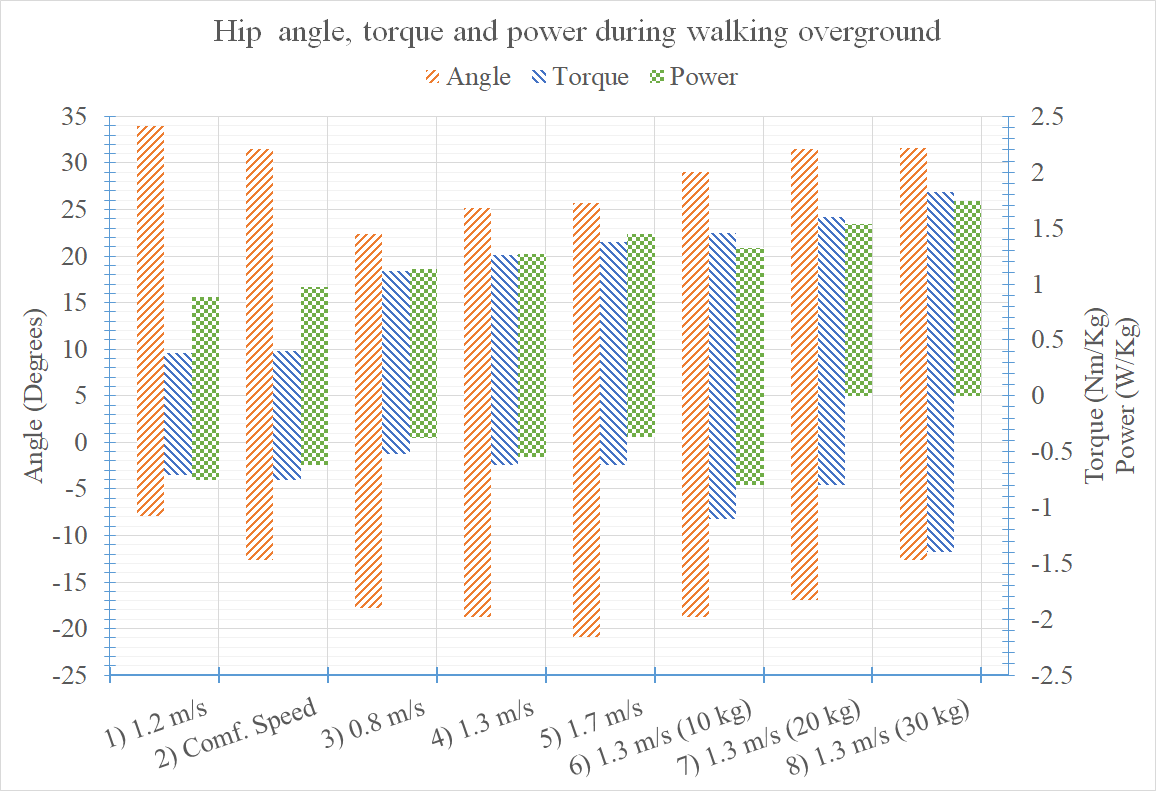
\includegraphics[width=\textwidth]{HipKKPWalkingExcel.png}
        \caption{Data compiled from several experiments of the hip joint for walking over ground activities. The weight next to the name of some activities dictates the load carried by the subjects during the experiment. The torque and power are presented in the same axis since their values share the  same order of magnitude \cite{solis2017characterization}. The gait analysis studies are as follows: (1) \cite{bovi2011multiple}, (2) \cite{lee2008biomechanics}, (3-8) \cite{han2011biomechanical}. }
        \label{fig:HipKKPWalking}
    \end{subfigure}
    \hfill
    \begin{subfigure}[b]{0.75\textwidth}
        \centering
        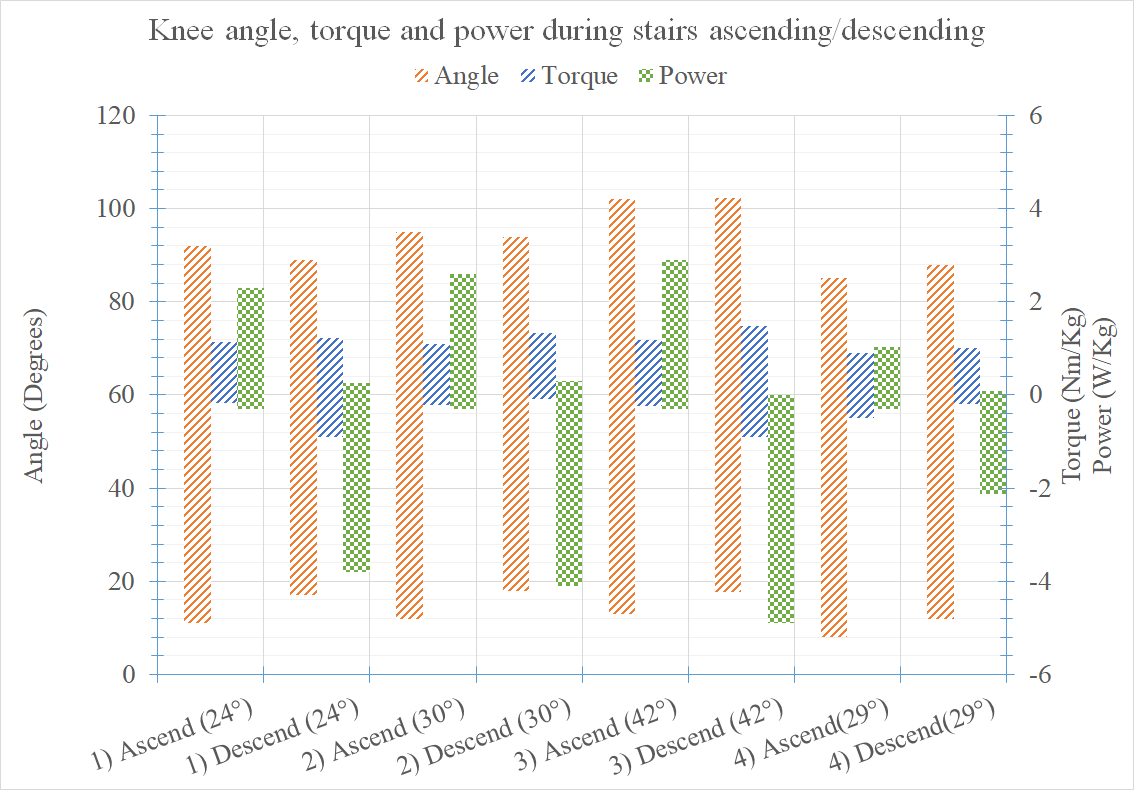
\includegraphics[width=\textwidth]{KneeKKPStairsExcel.png}
        \caption{Data compiled of the knee joint for several stairs ascending/descending experiments. The number enclosed in brackets represents the stairs slope. The parameters of torque and power are presented in the same axis since their values have the same order of magnitude. The gait analysis studies are as follows: (1) \cite{riener2002stair}, (2-4) \cite{reid2007knee}. }
        \label{fig:KneeKKPWalking}
    \end{subfigure}
    \caption{Visualization of gait analyses data using clustered-stacked bar charts \cite{solis2017characterization}. }
    \label{fig:clusteredMain}
\end{figure}

Different design guidelines can be extracted when visually analyzing other parameters together. For example, in \Cref{fig:KneeKKPWalking} , the parameters of the knee joint are now compared against many experiments of stairs ascending/descending. Now, the main feature is not the range of motion of the knee, but the characteristics of the torque values. They appeared mirrored, in other words, the torque values required for descending stairs are of similar in magnitude but opposite in direction. Also, the amount required for ascending stairs is generally twice as much as the amount required for descending stairs. The latter illustrates an optimization opportunity. When designing a wearable robotic device for human for human assistance, the actuator is chosen to satisfy a certain torque range of a particular activity. Without the characterization of the parameters performed, the actuator is most likely to be oversized to comply with the most demanding part of the activity. However, a different approach could be proposed: agonist-antagonist actuators; a technique implemented in several wearable robotic devices which at the same time complies with the actual functionality of the human skeletal muscle system.

Another useful way of extracting design guidelines from the gait analyses is to plot the range of a specific parameter against different ADL. At the best of our knowledge, this approach has only been documented once in \cite{rowe2000knee}, where the range of motion of the knee joint is compiled into a chart for 11 different ADL. This concept, illustrated in \Cref{fig:HipTorqueRange}, can provide insight of two important design parameters. On the one hand, the actuators meant for this application must be able to deliver torques in both directions of rotation, i.e. clockwise and anti-clockwise. On the other hand, the selected actuation technology must meat the torque requirements, specified in the \Cref{fig:HipTorqueRange}, of the activity or activities of interest. \Cref{fig:HipTorqueRange} was constructed using the mean range of the hip joint torque during different activities \cite{bovi2011multiple,lee2008biomechanics,han2011biomechanical,protopapadaki2007hip,riener2002stair,mcintosh2006gait,roebroeck1994biomechanics,mak2003joint}.

\begin{figure}[htbp!]
    \centering
    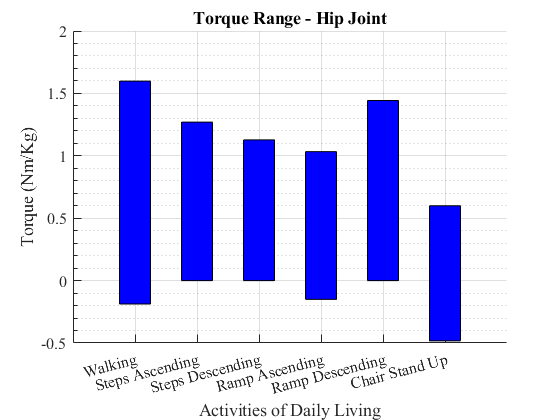
\includegraphics[width=0.8\textwidth]{HipTorqueRange.png}
    \caption{Illustration of the range values of the torque during several activities. The values for the maximum and minimum torque are mean values obtained by averaging the data of all the different gait analysis experiments enclosed in one main activity. \cite{bovi2011multiple,lee2008biomechanics,han2011biomechanical,protopapadaki2007hip,riener2002stair,mcintosh2006gait,roebroeck1994biomechanics,mak2003joint,solis2017characterization} }
    \label{fig:HipTorqueRange}
\end{figure}

Another alternative of visual representation of the data can be done by grouping the range of a specific parameter and comparing it with any of the subjects' physical characteristics, e.g. the age range. This is illustrated in \Cref{fig:KneeRangeAge}, where the dependency of the subjects' age with the knee range of motion is evidenced. The colour code used in \Cref{fig:KneeRangeAge}, the age ranges and knee ranges of motion are presented in \Cref{tbl:KneeRangeMotionage}. The chart shown in \Cref{fig:KneeRangeAge} concentrates the data from three different gait analyses, in which six age groups are contained. The approach used in \Cref{fig:KneeRangeAge} is to overlap areas of different colours, each area represents the range of motion of the knee for a specific age range. The area in which several areas intersect can be appreciated due to the enabled transparency property. Nevertheless, the areas where three and two areas are intersected are manually highlighted by a surrounding solid line and dotted line respectively, to improve their visualization. This simple intersection of areas can provide information regarding the required range of motion to be delivered by the wearable robotic device, depending the sector of the population focused on.
For example, if a wearable robotic device was aiming to assist the population sector aged from 50 to 70 years old, then a range of motion of the knee joint from 5 to 63 would be enough to cover the mentioned population. The later range of motion is taken from the triple intersection of areas illustrated in \Cref{fig:KneeRangeAge}, which can provide a certain degree of confidence since three different clinical studies were compared. This approach can be used to compare other characteristics, e.g. subject's weight against torque. Summarizing, the areas overlapping approach can provide guidelines to avoid oversizing of the wearable robotic device to be developed by analysing the intersection of different areas which ultimately provides a degree of confidence when deciding design parameters.

\begin{table}[htb!]
\caption{Colour code used in \Cref{fig:KneeRangeAge} for each combination of age range and knee range of motion. The knee range of motion is provided in degrees \cite{solis2017characterization}.}
\label{tbl:KneeRangeMotionage}
\begin{tabular}{c|c|c|c}
\hline
Colour Code & Knee Range of Motion (\degree{}) & Age Range (Years) & Clinical Study \\
\hline
Red         & 2.2 - 67.4               & 49 - 90           & \cite{rowe2000knee}       \\
Green       & 5 - 66.5                 & 6 - 17            & \cite{bovi2011multiple}        \\
Blue        & 4.5 - 63.5               & 22 - 72           & \cite{bovi2011multiple}           \\
Yellow      & 0 - 69                   & 18 - 30           & \cite{lee2008biomechanics}        \\
Magenta     & 0 - 69                   & 50 - 70           & \cite{lee2008biomechanics}     \\
Cyan        & 8 - 63.6                 & 23 - 27           & \cite{han2011biomechanical}    \\  
\hline
\end{tabular}
\end{table}

\begin{figure}[htb!]
    \centering
    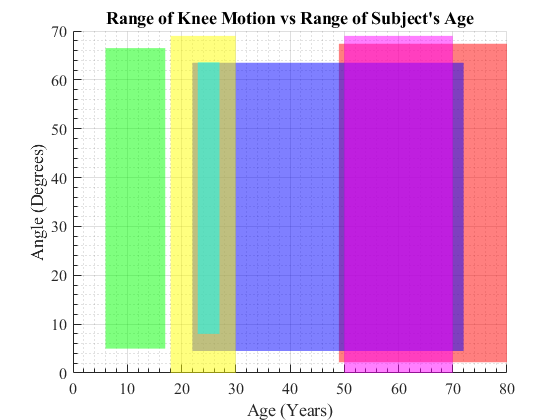
\includegraphics[width=0.7\textwidth]{KneeRangeMotionAge.png}
    \caption{Chart illustrating the comparison between subjects' age and the knee range of motion during walking over ground. The areas surrounded by solid lines and dotted lines represent the intersection between three and two areas, respectively. The overlapping squares highlight the great similarity among the range of motion despite subjects' age. The data used to create this chart is presented in \Cref{tbl:KneeRangeMotionage} \cite{solis2017characterization}. }
    \label{fig:KneeRangeAge}
\end{figure}

In this section the process of characterizing the human lower limb kinematics and kinetics parameters during some ADLs, was described. The relevant information provided in gait analysis experiments was described, as well as possible challenges when extracting it. Data compiled for the activities of walking, ascending/descending stairs, ascending/descending ramps and chair standing up were presented in the form of clustered stacked bar charts. This type of chart allowed quick and easy detection of similarities between several clinical trials of the same activity. In contrast, the spotted differences, as the ones for the knee torque values during ascending/descending stairs, are indicators for optimization opportunities where instead of using a single actuator to satisfy the torque range, an agonist-antagonist system could be more suitable.

The reliability of the data can also be observed using the type chart of overlapping areas with subjects' age ranges against the knee ranges of motion. In other words, the specific ranges in which the data from different experiments overlaps, gives a measure of consistency which can be used to tailor the developed wearable device coverage. 

The chart style with ranges of motion versus activities, facilitates the choice of the actuator type and dimension (depending on the activities of interest). The styles used to represent the charts was kept as simple as possible while providing useful information about the KKP. However, more complex plotting methods can be used. Finally, a total of 12 charts were produced in Excel\textregistered{} using the compiled data from the gait analyses. In favour of keeping the length of this section adequate, only two out of the 12 charts were included in here. The remainder charts were moved to the \Cref{appendixA}.

\section{The Muscle-tendon Component} \label{sec:muscle_tendon}

Having defined the terminology involved in the biomechanics of the human skeletal muscle system, and characterized the kinetic and kinematic parameters of its lower limb, this section now focus on describing the muscle-tendon component from a mechanical point of view. 

In the literature, the mechanical model commonly used to describe the mechanical behaviour of the muscle-tendon component is the Hill's model \cite{hill1938heat}. This model is considered to be the most representative of all \cite{zhang2012sma}. Hill's model describes the skeletal muscle as a three elements system, which contains a contractile element, a passive element, and a series element. The contractile element (CE) represent the muscle fibres in charge generating the contractile forces, the parallel element (PE) is formed by the tissue surrounding the muscle which prevents it from overstretching, and the series element (SE) represents the human tendon, as illustrated in \Cref{fig:hillModel}.

\begin{figure}[htb!]
    \centering
    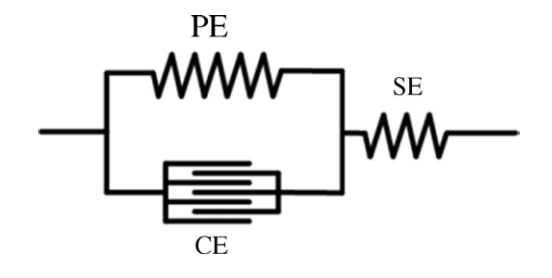
\includegraphics[width=0.5\textwidth]{HillModel.png}
    \caption{Hill's model of the skeletal muscle. The contractile element (CE), the parallel element (PE) and the series element (SE) are shown \cite{hill1938heat} }
    \label{fig:hillModel}
\end{figure}

Hill's model makes the important assumption of considering the SE to be purely elastic, i.e. the deformation of the element is entirely dependent to the force applied to it. Nevertheless, the non-linear viscoelastic properties of the human tendon are acknowledged in his work. The latter simplification is a common practice among studies of the skeletal muscle system because the muscle and tendon are studied as a whole (muscle-tendon component) \cite{zajac1989muscle}. Evidence of the actual benefits of this simplification is found in the literature for the field of robotics exoskeletons. The complex muscle-tendon model developed in \cite{lloyd2003emg}, considered the viscoelastic properties of the human tendon to estimate forces and joint torques in real time. The model achieved high accuracy at the cost of high computational load. In an attempt to reduce the computational load, the assumption of an infinitely stiff tendon was made which proved to be reliable as well \cite{sartori2009stiff}.

In a similar way, developments in the field of soft robotics which are inspired in the skeletal muscle system functionality are also based in Hill's model, as highlighted in \Cref{sec:SoftActuation}. Commonly, springs [13] or Bowden cables [44] are implemented as the SE of the muscle-tendon model. Nevertheless, the fact is that the human tendon has viscoelastic properties [76]. At the time of starting this research, the documented works in the literature were mainly focused on developing and testing soft materials to be used as the contractile element in a soft artificial muscles. The latter, previously identified as a research opportunity, indicates that the viscoelastic properties of soft materials have not been studied with the aim of developing a soft artificial tendon, which in combination with current soft artificial muscle could deliver better performance is soft robotic applications for human assistance.

The first step towards the investigation on the potential benefits of adding viscoelasticity, in the form of a soft SE, to soft actuators is described as follows. As a starting point,the mechanical properties of the human tendon must be investigated. Due to the large contribution of the knee joint in the ADL, we have focused our investigation in this joint of the human lower limb. Subsequently, the selection and characterization of many soft materials with mechanical properties similar to the human tendon, is proposed. The extracted properties from the soft studied soft materials and from the human tendon are compared against each other. This comparison analysis has the potential of providing evidence on the benefits and disadvantages of implementing a viscoelastic element as the way to transmit tensile forces in soft orthoses and soft exosuits.

\subsection{Viscoelasticity of the Human Tendon} \label{sec:viscoelasticity}

Tendons are connective tissue that links muscles with bones. As previously mentioned, the human tendon has a non-linear viscoelastic behaviour. This means that the deformation experienced by the material when a force is applied to it, is not proportional to the force through the whole range of possible deformations, and also that it is dependent on the history of previous deformations. At rest, the collagen fibres (core components of tendons) are in a relaxed wavy state. When the tendon experiences a tensile force, the collagen fibres are easily stretched and realigned, opposing little resistance to deformation. However, when the collagen fibres are completely stretched they begin to offer more resistance to deformation which is proportional to the applied force. Finally, fibres can be stretched to their limit and failure of the tendon will occur \cite{nordin2001basic}. This non-linear response to the applied deformation is better explained in \Cref{fig:tendonSS} where the characteristic S-shape curve for tendon stress-strain graphs is appreciated.

\begin{figure}[htb!]
    \centering
    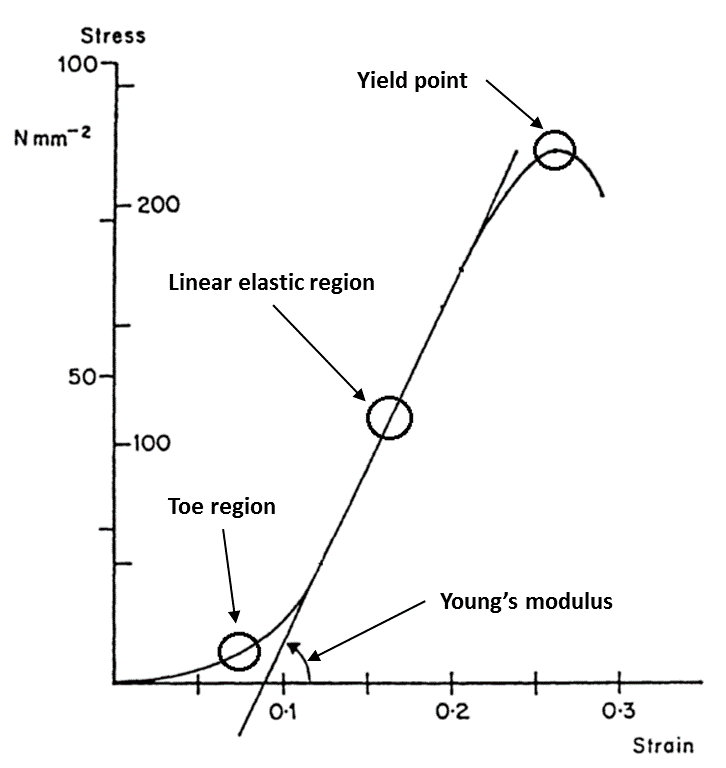
\includegraphics[width=0.6\textwidth]{TendonStressStrain.png}
    \caption{Tendon stress-strain curve. The toe region represents the interval where collagen fibres offer little resistance to deformation. The linear elastic region is when collagen fibres are stretched and start offering a linear behaviour. From the slope of this region, the Young's modulus can be extracted. The yield point is represented by the applied stress which cause plastic deformations on the tendon. Failure occurs beyond this point, where stress abruptly goes down as deformation continues. Image adapted from \cite{maurel1998biomechanical}. }
    \label{fig:tendonSS}
\end{figure}

The stress-strain curve in \Cref{fig:tendonSS} illustrates the mechanical properties of a human tendon. The stress is described as the tensile force per cross-sectional unit area experienced by the tendon. This stress causes the tendon to elongate (deform). In the chart, the elongation is represented as the strain, which is the tendon deformation as a percentage of its original length. Along with the stress-strain curve, the force-elongation curve is also used to visualize the mechanical properties of tendons. These experiments are performed in a static state, i.e. the strain rate is the same throughout the whole experiment. Therefore, they do not provide any information about the viscoelastic properties of the tendon.

Viscoelastic materials exhibit both elastic and viscous characteristic. Viscosity describes a fluid's resistance to flow, the more viscous a fluid is, the more slowly will flow and vice versa. The latter suggest a time-dependent behaviour. In the case of viscoelastic materials, this time-dependent behaviour is shown when subjecting the material to different rates of strain or deformation. For example, the stress-strain curve of the human tendon, illustrated in \Cref{fig:tendonSS}, would have a greater slope in the elastic region if a greater strain rate is applied. The viscoelastic behaviour of the human tendon can be analysed with the following mechanical tests: stress relaxation, creep (deformation over time) and hysteresis \cite{nordin2001basic}.

During the stress relaxation experiment, the tendon is subjected to a constant deformation (length remains the same throughout the whole experiment). To avoid plastic deformations, i.e. incorrect measurements, the parameter of deformation for this experiment must not exceed the linear region of the material. The initial force/stress triggered as a response of the applied deformation will decrease over time (relax) until reaching equilibrium. From this experiment a chart of force against time is generated (\Cref{fig:tendonSR_Creep}). In a similar way, in the creep experiment a constant force, avoiding plastic deformations, is applied to the material. The material will creep as time pass, in other words, the deformation caused by the applied force will increase over time until reaching equilibrium. A chart of deformation against time is generated (\Cref{fig:tendonSR_Creep}). Finally, during the hysteresis experiment the tendon is subjected to cyclic tests where a load is applied up to a certain stress level and then released (unloading). The tendon behaviour shows two different paths, one for loading and one for unloading. Due to the time-dependent behaviour of viscoelastic materials, each cycle will generate different load-unload paths since the time interval for each cycle to be executed are intentionally defined to prevent the material of reaching equilibrium (\Cref{fig:tendonHysteresis}).

\begin{figure}[htb!]
    \centering
    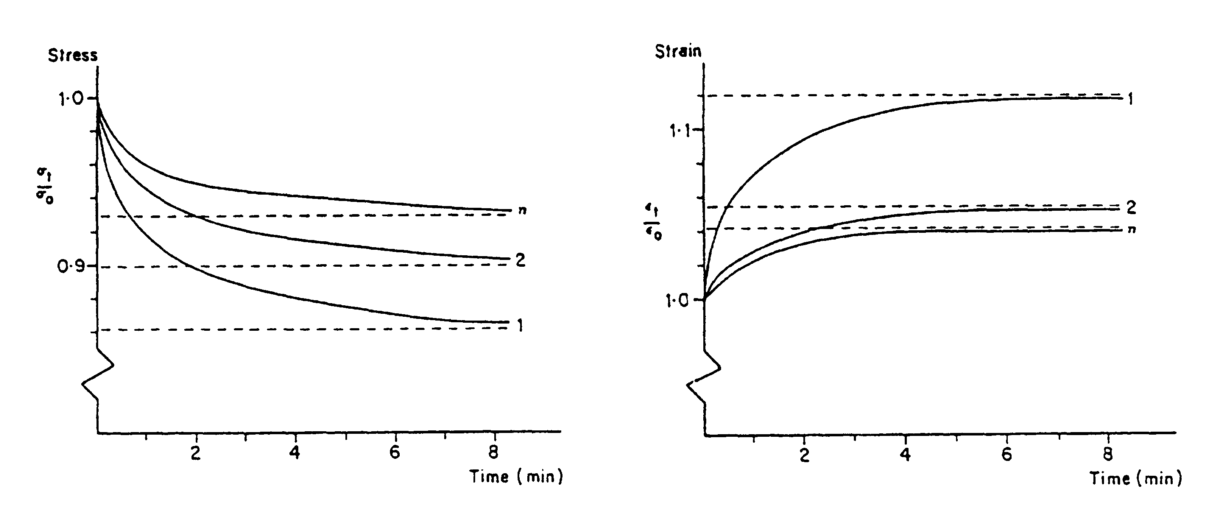
\includegraphics[width=\textwidth]{TendonSR&Creep.png}
    \caption{Tendon curves for the experiments of stress relaxation (left) and creep (right). The experiments were executed several times under the same conditions, the curve labelled \textit{n} illustrates the tendon reaching a steady state where repeatability between experiments is achieved. Image reproduced from \cite{maurel1998biomechanical} }
    \label{fig:tendonSR_Creep}
\end{figure}

\begin{figure}[htb!]
    \centering
    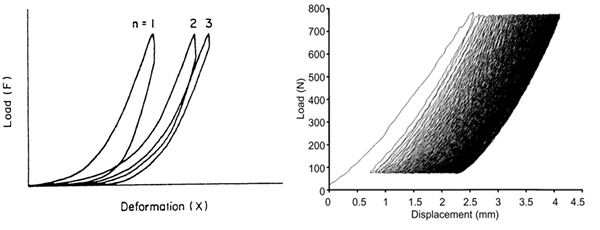
\includegraphics[width=\textwidth]{TendonHysteresis.png}
    \caption{Hysteresis of the human tendon. The chart on the left shows both loading and unloading paths for few cycles, whereas the chart on the right shows 200 loading-unloading cycles. The hysteresis of the tendon, i.e. the area under the curve, is smaller for each new cycle. The preconditioned state of the tendon is reached for cycles above 50, i.e. stop changing. Left and right images taken from \cite{maurel1998biomechanical,schatzmann1998effect} respectively. }
    \label{fig:tendonHysteresis}
\end{figure}

When performing mechanical experiments to find the tendon properties at failure, the obtained results are different between a preconditioned and an unconditioned tendon, as proved in \cite{schatzmann1998effect}. This effect is illustrated in \Cref{fig:tendonSR_Creep} as well, for both experiments, the tendon relaxation and creep are smaller for each new testing cycle until reaching an equilibrium state, i.e. the preconditioning state. The previous set of experiments is useful to characterize the non-linear viscoelastic properties of tendons and soft materials. Therefore, to perform the comparison analysis mentioned in \Cref{sec:muscle_tendon}, the soft materials of interest must be characterized using some of these mechanical tests. The study of the creep and hysteresis is out of the scope of this research. Instead, the tensile strength and stress relaxation is analysed. The selection criteria for the synthetic soft materials to be used is explained in next section.

\section{Soft Materials to Match the Properties of the Human Tendon} \label{sec:softMaterials}

The selection of the soft material to be implemented was based on the literature about tendon reconstruction applications. A comprehensive review about the usage of synthetic materials in tendon reconstruction is made by Andullah in \cite{abdullah2015usage}, where the most common materials used as artificial tendons and for tendon reconstruction, are reported as: carbon, polyethylene terephthalate (polyester), polytetrafluoroethylene, among others. The latter suggest that polymers are highly compatible with the human skeletal system and have similar mechanical properties as the human tendon. This assumption is further verified in the study performed by Duenwald et al. in \cite{duenwald2009viscoelastic}, which is about the viscoelastic relaxation and recovery of the human tendon. In this work, the high density polyethylene was tested to find great similarities between this material and the mechanical properties of the human tendon. In fact, the viscoelastic properties of the human tendon during loading and unloading are similar to the ones found in polyethylene. However, high density polyethylene is not able to sustain high strains without suffering plastic deformations nor it has a very fast elastic response.

Among the current developments in soft orthoses, silicone rubber is a common choice, due to its high compliance, high elasticity and softness. Silicone rubber is usually implemented to create inflatable elements, but it is also known to have non-linear elastic properties, as reported in \cite{roylance2008mechanical}. These findings suggest that the limitations of polymers, in terms of its elasticity, could be circumvented when combined them with elastomers, such as rubber. A material with the latter characteristics, is known as a composite materials. Many composite materials are created by injecting polymer particles, such as the previously mentioned polyethylene, into a rubber mixture. Thanks to the advances in manufacturing of composite materials, there is a wide variety of commercially available materials that fit with the requirements of this research. Due to the latter information, the selection of the soft materials to be studied in this work are from the family of composite materials, as follows: Polyethylene Rubber, Ethylene Polypropylene, Natural Rubber with Polyester, Natural Rubber, Silicone Rubber, Fluorocarbon Rubber, and Nitrile Rubber. All the materials were acquired from RS Components UK\textregistered{}, with the exception of the Natural Rubber, which was acquired from CoreZone Sports\textregistered{} in the form of resistance bands of different thickness. Finally, the characterization process and more details about the materials are provided in \Cref{ch:characterizationSoft}.

\newpage

\section{Modeling Techniques for Soft Materials} \label{sec:modelingTechniques}

In \Cref{sec:gaps}, the lack of a reliable model to predict the mechanical behaviour of soft materials was identified as a gap in the body of knowledge. This limitation plays a crucial role in the process of investigating the potential benefits of mimicking the human skeletal muscle functionality, and so it is addressed in this section. 

Most of the documented soft robotic applications use soft materials from the family of thermoplastic elastomers (TPE). These type of materials are known to have a non-linear stress response, low stiffness, high deformation lengths, and a time-dependent and temperature-dependent response \cite{Bauman2008}. These mechanical properties are similar to the ones found in biological skin or muscle tissue, which is why soft materials are being implemented in soft robotic applications, despite of the many challenges. However, it is imperative to have a reliable modelling technique to fully take advantage of the latter mechanical properties.

At this point, it has been established the complexity of the mechanical behaviour of soft materials, such as TPE. In general terms, the stress response of these materials is nonlinear and viscoelastic. The most commonly modelling technique used when dealing with viscoelastic materials is the development of a mathematical constitutive model. Many authors, choose the Linear Viscoelastic Models (LVM) as the starting point \cite{xu2014mathematical,tirella2014strain,lu2017constitutive,ciniello2017identifying}. This has been also the case when modelling the mechanical behaviour of biological tissues \cite{sanjeevi1982viscoelastic}. The LVM are a set of mathematical models which use two basic components, a spring and a damper, in different configurations and quantities to describe the viscoelastic mechanical behaviour of materials \cite{roylance2001engineering}. Inside this family of mathematical models, there are a couple of them which are considered able to describe the viscoelastic behaviour of any material, as long as the required number of parameters of the model is met. This immediately impose the restriction of having enough computational power to deal with the model complexity when high accuracy is required.

At this stage of the research, the implementation of soft materials in soft robotic applications is scarce. Most of the effort is focus on improving the traditional series-elastic actuator (SEA) by replacing its elastic element, commonly a metallic spring, with a viscoelastic material, such as rubber. SEA are from the family of cable-driven actuators and are commonly based on electric motors. The main feature of these actuators is that they have an elastic element between the actuator and the load. SEA have greatly impacted the field of robotics, specifically in legged robotics and powered orthoses, due to many benefits such as: greater shock tolerance, low output impedance, passive energy storage, and more accurate force feedback \cite{pratt1995series,pratt2004series,au2008powered}. Almost two decades after Pratt et al. documented the first SEA prototype, SEA are now considered a mature actuation technology, and as such, they have a well-defined trade-off, caused by the fixed stiffness provided by linear springs traditionally used. More often than not, variable stiffness is more suitable for the legged robots and powered orthoses. The latter limitation have been addressed by developing variable stiffness actuators \cite{groothuis2012vsaut}, using non linear metallic springs \cite{migliore2007novel}, and very recently by using viscoelastic materials, such as polymers and rubber \cite{rollinson2013design,parietti2011series,schepelmann2014compact}. However, these works, specifically the ones dealing with soft materials, are still facing the challenge of modelling the their mechanical properties. 

In \cite{parietti2011series}, where the concept of a series-viscoelastic actuator (SVA) is first mentioned, the modelling of the soft material is based on the Burger Model, one of the most complete LMVs, in combination with a controlling technique known as the state space observer. The accuracy of the system was found to be proportional to the complexity of the mathematical model used. The studied material in this work was a rigid-acrylic based photopolymer (FullCure720). The reported control system contained the viscoelastic model, the state space observer, and a cascaded force-velocity scheme, in other words, a very complex and well thought control system for a linear viscoelastic polymer. The developed SVA is illustrated in \Cref{fig:firstSVA}. 

\begin{figure}[htb!]
    \centering
    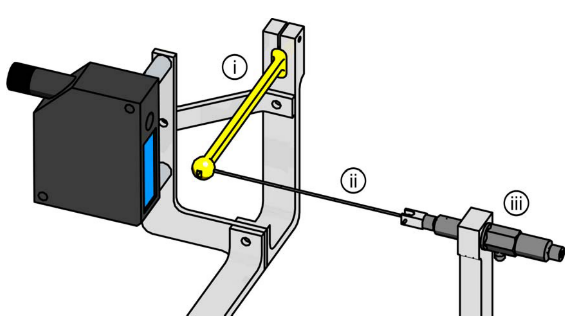
\includegraphics[width=0.6\textwidth]{FirstSVA.png}
    \caption{Series-viscoelastic actuator proposed by Parietti et al. The end effector is rigidly mounted on the revolving lever (i), which also supports the laser sensor. A Nylon line (ii) connects the end-effector handle to the high-precision piezoelectric force sensor (iii), which is fixed to a rigid support \cite{parietti2011series}.}
    \label{fig:firstSVA}
\end{figure}

Following this line of research, Rollinson et al. attempted to add viscoelasticity to a SEA, this time a soft material is used, natural rubber, instead of a rigid polymer \cite{rollinson2013design}. The developed SEA has a rotary spring. Two different types of rubber, and a type of neoprene, were studied. In here, the stress response of the materials is considered linear and instead, the hysteresis of the material is modelled (\Cref{fig:tendonHysteresis} in \Cref{sec:viscoelasticity}). Again, the modelling of the soft material is based on one of the LVM, the Standard Linear Solid (SLS) model, which is slightly less complex than the Burger model. Thanks to the proposed mechanical design for the rotary SEA, the reported stress response of the studied rubbers was surprisingly linear under a specific range of deformations. The authors concluded that more work is required to create better modelling techniques for the hysteresis and non-linear behaviour of soft materials like elastomers. The developed rotary spring is illustrated in \Cref{fig:rotarySoftSEA}.

\begin{figure}[htb!]
    \centering
    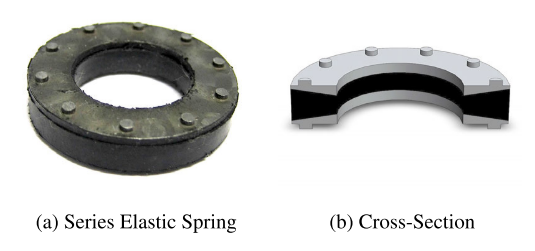
\includegraphics[width=0.6\textwidth]{RotarySoftSEA.png}
    \caption{Photo (a) and cross-section (b) of the developed soft rotary spring \cite{rollinson2013design}}
    \label{fig:rotarySoftSEA}
\end{figure}

Following a more traditional approach, Schepelmann et al. incorporated viscoelasticity in cable-driven SEA by using a rubber material as the elastic element, instead of the traditional metallic spring \cite{schepelmann2014compact}. In here, no LVMs are used, instead the nonlinear stress response of the rubber is simplified by fitting a second order exponential curve to the stress-strain curve to the material. The main motivation of this work is to tackle the limitations of SEA with non-linear springs (NLS), in where computer-aided manufactured (CAM) structures are used to define a known deflection trajectory of the spring, thus defining a torque trajectory. Essentially, CAM structures are able to relate the spring deformation with the generated torque, allowing the implementation of control systems. This work successful validated the suitability of rubber to be incorporated as part of a SEA However, under the limited range of testing parameters, the authors were not able to observe any velocity-dependency on the stress response of the rubber. In the conclusions, a state space observer is recommended to improve the accuracy of the reported forces transmitted by the the soft material, i.e. to allow the controller to compensate the hysteresis and nonlinear stress response of the material.

\begin{figure}[htb!]
    \centering
    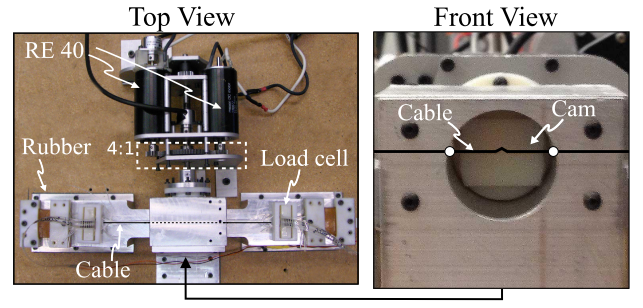
\includegraphics[width=0.6\textwidth]{SoftSEACAM.png}
    \caption{Benchtop setup for rubber characterization and observer testing. The load side of the rubber is fixed. Load cells in-line with the rubber give rubber force measurements for testing. The choice of electric motors and transmission is illustrated \cite{schepelmann2014compact}}
    \label{fig:softSEACAM}
\end{figure}

In an attempt to relieve the controller for such load, the latter work was continued by Austin et al., this time focused on developing a modelling tool to better model the complex behaviour of rubber \cite{austin2015control}. In here, the complexity of modelling the nonlinear and strain-dependent stress response of soft materials is addressed, for the first time, by upgrading the SLS model without greatly increasing its complexity. A piecewise linearization method is implemented, to transform the equilibrium spring in the SLS model into several springs in parallel which sequentially engages proportion to the strain applied to the material. The developed mathematical model is called the Standard Linear Solis model with Strain-Dependent Stiffness. (Std. Lin. SDS). Although, the SLS is not the most complete model among the LVM, the reported accuracy of the developed model is impressive. The control system implemented a state space observer, as well, which able to correctly estimate the torque generated by the rubber spring. However, despite the large improvement in accuracy obtained by the developed Std. Lin. SDS, the hysteretic properties of the rubber  lead to instability at higher frequencies, suggesting that there is still work to be done in this field.

\section{Summary}

In this chapter, the terminology on the biomechanics of the human lower limb is presented. Subsequently, the characterization of the kinetic and kinematic parameters of the hip, knee and ankle joints is performed by reviewing many clinical trials about gait analysis of the lower limb. The collected data had the potential to be used as design guidelines when developing robotic devices targeted for human assistance. Therefore, many visualization techniques were proposed and analysed in this context. The latter work resulted in a published conference paper (\Cref{sec:characterizationKKP}). 

In line with the aim of this research of investigating the potential benefits of mimicking the human skeletal muscle system functionalities in soft robotic applications, the main element of the latter system, the muscle-tendon component, was described in \Cref{sec:muscle_tendon}. In the literature, the works that implement the concept of mimicking the muscle skeletal system are focused on the contractile element of the muscle-tendon component, i.e. the muscle. Very little attention is paid to the series element, the tendon. Furthermore, it was found that the viscoelasticity present in the human tendon, and biological tissues in general, is also present in certain polymers and composite materials. Therefore, the proposal of performing a comparison analysis between different off-the-shelf composite materials and the human tendon mechanical properties is presented. This comparison analysis will contribute to the aforementioned aim of the research. The first step to perform this comparison analysis is to characterize the mechanical properties of the selected materials, listed in \Cref{sec:softMaterials}. This is described in \Cref{ch:characterizationSoft}.

Recently, attempts of adding viscoelasticity to well-established actuation technologies have been done. Specifically, viscoelasticity has the potential to address many of the limitations found in series-elastic actuators. The available literature on the subject is scarce but very well documented. In general, the reviewed works face a common challenge, the modelling of the viscoelastic properties of the materials used to accurately estimate their reaction force or torque. Rubber is the most common choice in these applications. Almost all of the documented works are based on a model-driven approach, based on the Linear Viscoelastic Models, for the extraction of the material. However, the work performed by Austion et al. in \cite{austin2015control}, is the first attempt to upgrade the potential of the LVMs by applying a piecewise linearization method. The authors succeeded in developing a mathematical model, called the Standard Linear Solis model with Strain-Dependent Stiffness. (Std. Lin. SDS) which achieve higher ac curacies than traditional models. However, even with the aid of controlling techniques such as the state space observer, the implemented control system is still unable to account for properties of the material, such as hysteresis and the velocity-dependency in their stress response. Nevertheless, the developed mathematical model has the potential to be upgraded further by using the same piecewie linearization method but on a more complex LVM. This idea is further explored in an attempt to develop a reliable modelling tool for the prediction of the mechanical properties of soft materials. This is presented in \Cref{sec:ChapterModellingLVM}.



\include{Chapters/Chapter_2b/Chapter_2b_File}
\chapter{Characterization of the Soft Materials Behaviour} \label{ch:characterizationSoft}

\textbf{ \huge To-Do List}

Explain characterization process following a systematic approach:
\begin{itemize}
    \item In the introduction:
    \begin{itemize}
        \item[$\cross$] Mention the two performed mechanical tests and general parameters
        \item[$\cross$] Justify the reason why those tests were performed
        \item[$\cross$] List the soft materials analyzed
        \item[$\cross$] Describe how the specimens to test were extracted from the material sheets
        \item[$\cross$] Illustrate the specimens layout, recommended in the test standard, using my own SolidWorks drawing with dimensions
    \end{itemize}
    \item Tensile strength test:
    \begin{itemize}
        \item[$\cross$] Describe the test
        \item[$\cross$] List the parameters extracted
        \item[$\cross$] Describe the load-deformation curve
        \item[$\cross$] Compile in a table the deformation rate used for each material (this table can be placed instead in the section where the different datasets used to train the neural networks is mentioned).
        \item Describe the criteria used to decide how much to smooth the raw data
        \item Illustrate the obtained load-deformation curves
    \end{itemize} 
    \item Describe the stress relaxation test. Mention the parameters collected. Compile in a table the deformation to which each material was held during the test. Mention that initially the test duration was longer than the one being used for fitting the mathematical model.
    \item Describe now the pre-processing done to the collected raw data. Several conditions were established to decide how much to smooth the raw data.
    \item Present the obtained stress relaxation curves
\end{itemize}

Things to explain
\begin{itemize}
    \item Allowable attenuation of max value is 5 percent
    \item (Done) Consider cell resolution for limiting the amount of attenuation in the smoothing algorithm to the right amount. (The load cell used provides accurate measurements up to 1/500 of its capacity, i.e. for a load cell of 50 kN the smallest accurate measurement is 100N. All the soft materials implemented have load values in the range of 1 to 100 N. Therefore, using the accuracy parameters of the load cell as a guide is not possible.)
\end{itemize}

\section{Introduction}

In this chapter, the characterization process of seven rubber-based (elastomers) soft materials is presented. The selected soft materials are: ethylene polypropylene rubber (EPR), Fluorocarbon rubber (FR), nitrile rubber (NR), natural rubber with polyester (NatR),  polyethylene rubber (PR), silicone rubber (SR) and  off-the-shelf resistance bands of different thicknesses which are made of 100\% Natural Rubber (NatR100). Here in parentheses, the code names used for each material in future sections is presented.

In the first section, the mechanical properties of the selected elastomers is described and categorized as elastic and viscoelastic (time-dependent) properties. In the second section, the mechanical tests of tensile strength and stress relaxation, used for the characterization process, are described. The description of the algorithm implemented in Matlab to filter out the noise embedded in the experimental data is also included in this section. In the third section, a comparison analysis between the mechanical properties of the studied soft materials and the mechanical properties of the main tendon involved in the motion of the human knee joint (Patellar tendon), is presented.

\section{Mechanical Properties of Soft Materials} \label{mechprop}

The soft materials studied in this work belong to the thermoplastic elastomer family. Elastomers are created by mixing a thermoplastic material, such as natural or synthetic rubber, with other materials, such as carbon and sulfur. This process is called vulcanization which creates cross-linked structures inside the material. Since elastomers are based on rubber, the terms elastomer and rubber are often used interchangeably. Elastomers are known to have non-linear stress response, low stiffness and to achieve high deformation lengths. Some elastomers can fully recover their shape after stretched many times their length. They are also known to exhibit both elastic and viscoelastic properties. The latter means the stress response of elastomers is also time-dependent \cite{Bauman2008}. The main mechanical properties of elastomers are described in following paragraphs.
\subsection{Elasticity}
Elasticity, or elastic behaviour, refers to the ability of a material to be deformed up to a certain length and completely recover its shape and dimensions when the load deforming it is removed. Elasticity also refers to ability of a material to comply with the law of constant proportionality between the stress and the strain, described by Hooke's Law. However, elastomers are not purely elastic materials and tend to have a nonlinear stress-strain response, i.e. they do not obey Hooke's Law over the whole range of strains in the sense that the proportionality between the stress and the strain does not remain constant. This typical non-linear behaviour in the stress-strain curve of elastomers is illustrated in Figure \ref{fig:tensile}.

\begin{figure}[hb!]
    \centering
    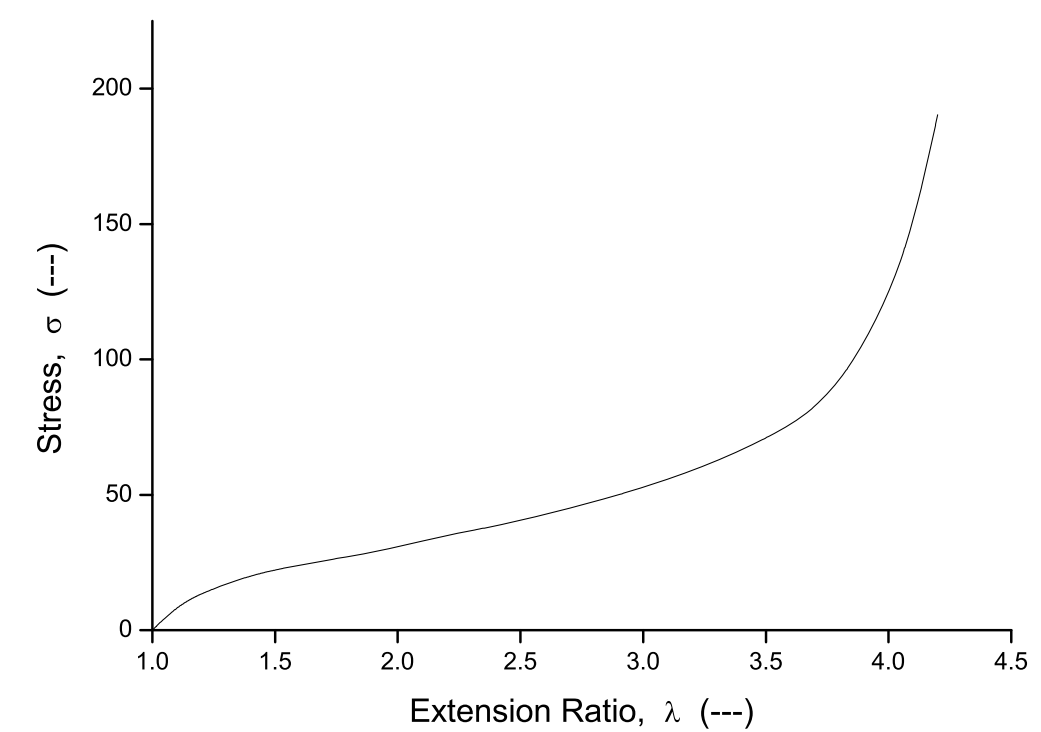
\includegraphics[width=0.7\textwidth]{TensileExample.png}
    \caption{Typical stress-strain curve of elastomers. \cite{Bauman2008}.}
    \label{fig:tensile}
\end{figure}

Elastomers are able to exhibit elastic behaviour up to a certain limiting load, known as the elastic limit. Beyond this limit the material is likely to undergo plastic or permanent deformation, this means the material will not recover its original shape completely. In some cases, the elastic limit is not easily visible from the stress-strain curve of a material and instead the proportional limit is used. The proportional limit defines the point in the stress-strain curve where the nonlinear response (change in the curve's slope) is first observed. Another way to delimit the elastic behaviour of a materials is using the yield strength which is defined as the maximum value on the curve or the first point in which an increase in strain occurs without an increase in strain \cite{ebewele2000}. These are some of the parameters that can be extracted from the tensile strength test and are useful to delimit the operating conditions of the materials.
\subsection{Viscoelasticity}
Viscoelasticity, is a property of some materials which are not purely elastic, do not fully obey Hooke's Law, nor purely viscous, do not fully obey Newton's Law, i.e. the stress is not proportional to the rate of change of the strain with time. In other words, the stress experienced by viscoelastic materials are dependent on both the amount and the speed of the strain applied to them. A purely elastic material is modelled, mechanically, as a spring; whereas a purely viscous material is modelled as a dashpot. By combining both of these elements it is possible to approximate the behaviour of a viscoelastic materials. These different combinations are known as the Linear Viscoelastic Models which will be described in latter sections. Finally, The time dependency of viscoelastic materials is appreciated in phenomenons such as creep, stress relaxation, hysteresis, the Mullin's Effect and in the Van der Waals forces.

Stress relaxation and creep are both time-dependent phenomenons observed in elastomers. On one hand, stress relaxation refers to the decrease over time of the stress experimented by a material when subjected to a constant strain (or deformation). On the other hand, creep refers to the increase over time of the material strain when subjected to a constant stress (or load). Understanding these phenomenons means understanding elastomers are composed of a network of molecular chains. Inside this network, entanglements form naturally. According to J. Bauman, stress relaxation is mainly caused by the slipping of these entanglements ultimately causing a loosening of force applied by the network of molecular chains. Stress relaxation and creep occur in both constant and cyclic deformations. Lastly, there are two mechanical tests designed to study these behaviours, from where it can be extracted the relaxation modulus and creep modulus of a material (\cite{oberg2016}). 

Hysteresis in a material is defined as the mechanical energy dissipated as heat when the material is undergoing deformations. This phenomenon is observed in a loading-unloading cycle, where the stress trajectory of the material while loading (extension) is different than the trajectory during unloading (retraction), as illustrated in Figure \ref{fig:hysteresis}. Hysteresis is mainly caused by internal friction of the molecular chain, also known as Van der Waals forces, in both elongation and contraction. Van der Waals forces are caused by the momentary bonding experienced between molecular chains that are close together. This constant making and breaking of bonds caused by deforming a material produces heat which ultimately becomes a mechanism to dissipate mechanical energy. This energy is represented as the enclosed area in Figure \ref{fig:hysteresis}. Stress relaxation and creep play a role in the amount of hysteresis experienced by a material in each consecutive loading-unloading cycle. The effect of hysteresis alone can be isolated by subjecting the elastomer to a conditioning process (preconditioning) in which it undergo several loading-unloading cycles until the stress response stops changing with every new cycle.

\begin{figure}[hb!]
    \centering
    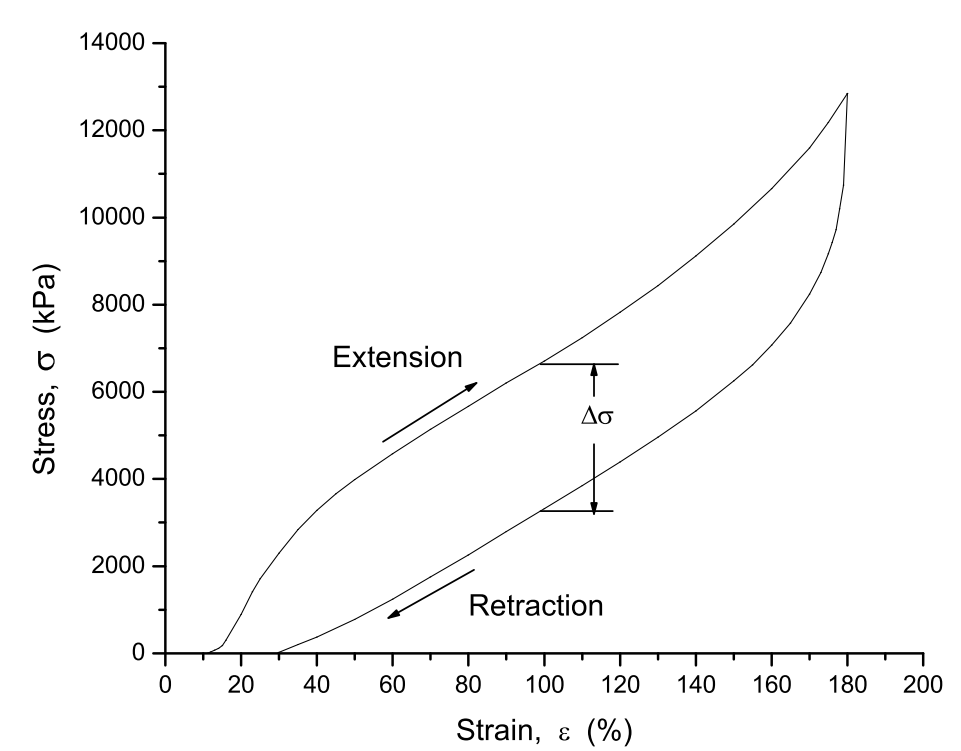
\includegraphics[width=0.7\textwidth]{HysteresisExample.png}
    \caption{Hysteresis in stress-strain curve. \cite{Bauman2008}.}
    \label{fig:hysteresis}
\end{figure}

The Mullin's effect is another important phenomenon to account for when studying the mechanical behaviour of elastomers. This effect refer to the breakage of tense molecular chains resulted from the manufacturing process of the material. Therefore, the very first time the material is subjected to deformations it exhibits a larger stress response in comparison to consecutive deformations. The latter is also referred to as a weakening of the material. This effect is more dramatic than the stress relaxation but can be easily avoided when preconditioning the material. Having defined the expected mechanical properties of elastomers, the mechanical tests of tensile strength and stress relaxation are described in the following section.

\section{Characterization Process}
In this section, the mechanical tests of tensile strength and stress relaxation, performed as part of the characterization process, are described. The tests are performed in an Instron 3369 Dual Column Testing System equipped with a 50 kN load cell, at room temperature (25 \degree C). The experimental data is expected to contain some noise due to the accuracy limitations of the available load cell. The algorithm implemented to filter this noise is described in SECTION . As previously mentioned, the elastomers selected for this research are: ethylene polypropylene rubber (EPR), Fluorocarbon rubber (FR), nitrile rubber (NR), natural rubber with polyester (NatR),  polyethylene rubber (PR), silicone rubber (SR) and  off-the-shelf resistance bands of different thicknesses which are made of 100\% Natural Rubber (NatR100). All the materials come in the form of a rectangular sheet. Laser cutting was used to extract individual specimens from each material sheet. In the Standard Test Method for Vulcanized Rubbers - Tension (ASTM D412), it is recommended to use five material specimens per test. Similarly, the recommended layout for the specimens, based on the thickness of the materials, is the Type C Dumbbell illustrated in Figure \ref{fig:specimenLayout} \cite{astmd412}.

\begin{figure}[hb!]
    \centering
    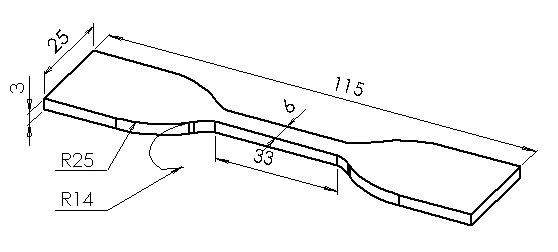
\includegraphics[width=0.6\textwidth]{SpecimenLayout.png}
    \caption{Specimen Type C Dumbbell Layout from the ASTM D412 \cite{astmd412}}
    \label{fig:specimenLayout}
\end{figure}

\subsection{Tensile Strength Test}

In a tensile strength test the material is loaded to failure at a certain deformation (strain) rate. The main purpose of this test is to extract the stress-strain curve of the material. From the stress-strain curve, the elastic properties of the material, such as stiffness, elastic modulus, ultimate strain, ultimate stress, elastic limit and yield strength, can be extracted. The stress-strain curve of elastomers (Figure \ref{fig:tensile}) has three main regions: the toe region, the elastic region, and the yield/failure region. In the toe region, the internal molecular chains of the material are misaligned, experiencing greater friction forces which greatly oppose to initial deformations. In contrast, when the molecular chains are aligned the friction forces decrease and the material deforms as a whole. The latter represent the elastic region, in which the slope of the curve (stiffness) is slightly smaller than in the toe-region. The elastic region of many materials exhibit a proportional or linear relationship between the stress and the strain. This is not the case for elastomers, where most of them exhibit a non-linear relationship. When the internal molecular chains have been elongated to its maximum length they demand higher forces to fail, this is observed as a peak in the load-elongation curve which also highlights the beginning of the yield/failure region \cite{Bauman2008}.

The tensile strength test performed in this work is in accordance with the Standard Test Method for Vulcanized Rubbers - Tension (ASTM D412) \cite{astmd412}. In here, it is recommended to elongate the material specimen until failure using a deformation rate of 500 mm/min, whenever possible. However, under certain circumstances where the previous deformation rate is not suitable, the test can be performed using the deformation rate of 250 mm/min. The latter was required for the silicon rubber, natural rubber and some resistance bands, where the gripper was not able to hold the material during the entirety of the test. In addition to the previous two deformation rates, a third one of 50 mm/min is used whenever possible. In summary, most of the materials are tested using at least two out of the three deformation rates of 50, 250 and 500 mm/min, to account for the deformation rate dependency, during the modelling stage, expected in the stress-strain curve of elastomers. The exact number of tests performed to each material is summarized in Table \ref{tbl:tensile_tests}.

\begin{table}[t]
    \centering
    \caption{Type and quantity of the different tensile strength tests performed. All the resistance bands are made of 100 \% Natural Rubber and are color coding depending on their stiffness.}
    \begin{tabular}{|C{0.3\textwidth}||C{0.2\textwidth}|C{0.1\textwidth}|C{0.1\textwidth}|C{0.1\textwidth}|}
    \hline 
    \multicolumn{5}{|c|}{Tensile Strength Datasets}\\
    \hline
    Type of Rubber & Thickness (mm) &   \multicolumn{3}{|c|}{ Deformation (mm/min)}\\
    \cline{3-5}
          &  & 50 & 250 & 500\\
    \hline
    Ethylene Polypropylene   &  1.5 & 16 & 0 & 5\\
    Fluorocarbon              &  1.5 & 9 & 8 & 5\\
    Natural with Polyester   &  1.5 & 10 & 5 & 0\\
    Nitrile                   &  1.5 & 7 & 7 & 5\\
    Silicone                  &  1.5 & 13 & 7 & 3\\
    Polyethylene              &  6 & 12 & 7 & 5\\
    \hline
    100\% Natural - Yellow  & 0.33, 0.42 & 1 & 6 & 1\\
    100\% Natural - Red  & 0.48, 0.52 & 0 & 8 & 0\\
    100\% Natural - Blue  & 0.64, 0.75 & 0 & 8 & 0\\
    100\% Natural - Green  & 0.97, 1.03 & 0 & 0 & 8\\
    100\% Natural - Black  & 1.17, 1.31 & 0 & 6 & 2\\
    100\% Natural - Orange  & 1.32, 1.49 & 0 & 5 & 0\\
    \hline
    \end{tabular}
    \label{tbl:tensile_tests}
\end{table}

One of the main parameters to extract from the obtained stress-strain curves is the elastic limit of each material. As previously mentioned in Section \ref{mechprop}, this parameter dictates the maximum amount of deformation a material can sustain without losing the ability to fully recover its original shape, i.e. its elasticity. Commonly, the proportional limit is used to approximate the location of the elastic limit, and by extension, the location of the elastic region. The proportional limit is the point in the curve where the proportionality between stress and stress becomes non-linear. It can be safely assumed that the elastic region of the material is located below this point. However, most elastomers do not have a clear elastic region due to their non-linear stress-strain curve, hence the proportional limit cannot be obtained. Under this circumstance, the elastic region of the material can be approximated using the yield strength of the material. The latter is defined as the first point in the curve where an increment in strain happens without and increment in the stress, hence the slope becomes zero or even negative \cite{astmd638}. In the scenario where the yield strength is difficult to extract, which is the case for most elastomers, the offset yield strength can be used as an alternative.

CONTINUE HERE(REMEMBER TO REVIEW PREVIOUS SECTION ABOUT PROPERTIES) - The calculation of the offset yield strength requires two parameters: the offset strain and the elastic modulus at a specific strain. In the literature, an offset strain of 2\% is recommended for plastics and elastomers (\cite{instron2019}). This recommendation is mainly to allow comparisons between different laboratories data and does not indicate a goodness of fit when approximating the elastic region or the yield point of a material. For the elastic modulus at a specified strain, the main recommendation is to select a portion at the beginning of the stress-strain curve in which a linear behaviour can be observed and apply a linear regression to this region to obtain the elastic modulus. In this work, the optimal strain range for the elastic modulus is obtained by trial and error. In summary, an offset strain of 2\% and an elastic modulus at 20\% strain were chosen to calculate the offset yield strength of all the materials which allowed us to approximate their elastic region and delimit their working conditions. 

Having defined these parameters, the first step to calculate the offset yield strength is to apply a linear regression to the first part of the curve (up to 20\% strain). The slope of this line represents the elastic modulus at the specified strain. The second step is to create a new line, starting from the specified 2\% offset strain, using the previously found elastic modulus as its slope. Finally, this line is projected up to the point in which it intersects the stress-strain curve. The stress and strain at this point represent the offset yield stress and the offset yield strain, respectively. Therefore, it is assume that beyond this point the material start undergoing plastic deformations. Similarly, it is assumed that the material is able to recover its original shape for all deformations found bellow the offset yield strain. Summarizing, the offset yield strength is illustrated in Figures \ref{fig:EPR} to \ref{fig:Nat100R} along with the initial part of the stress-strain curves of the studied materials for all the performed tensile strength tests. 
Furthermore, the elastic properties extracted from the stress-strain curves are reported in Table FILL.

\newpage
%The correct factor to fit to figures in the same line is 0.49
\begin{figure}[H]
    \centering
    \begin{subfigure}[b]{0.49\textwidth}
        \centering
        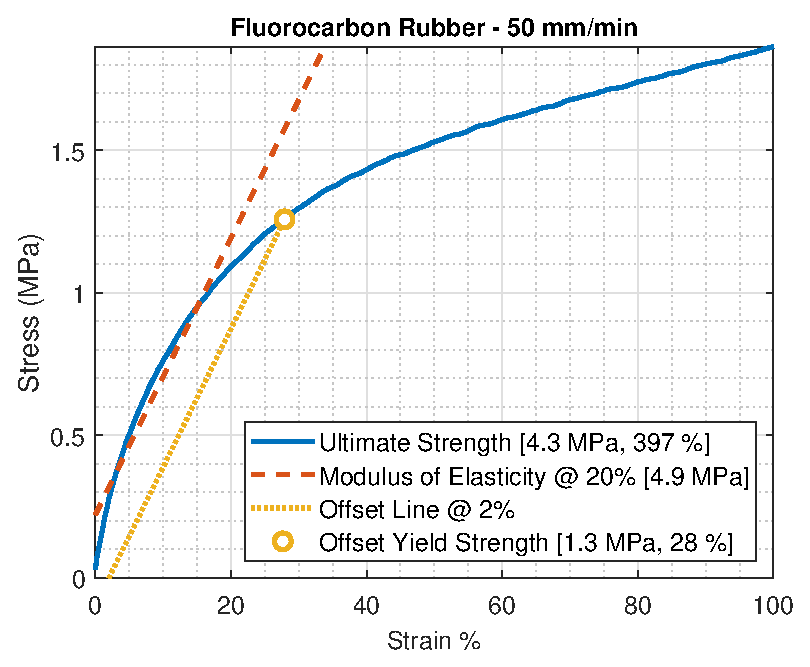
\includegraphics[width=\textwidth]{FR_disR50.eps}
        \caption{Caption}
        \label{fig:FR50}
    \end{subfigure}
    \hfill
    \begin{subfigure}[b]{0.49\textwidth}
        \centering
        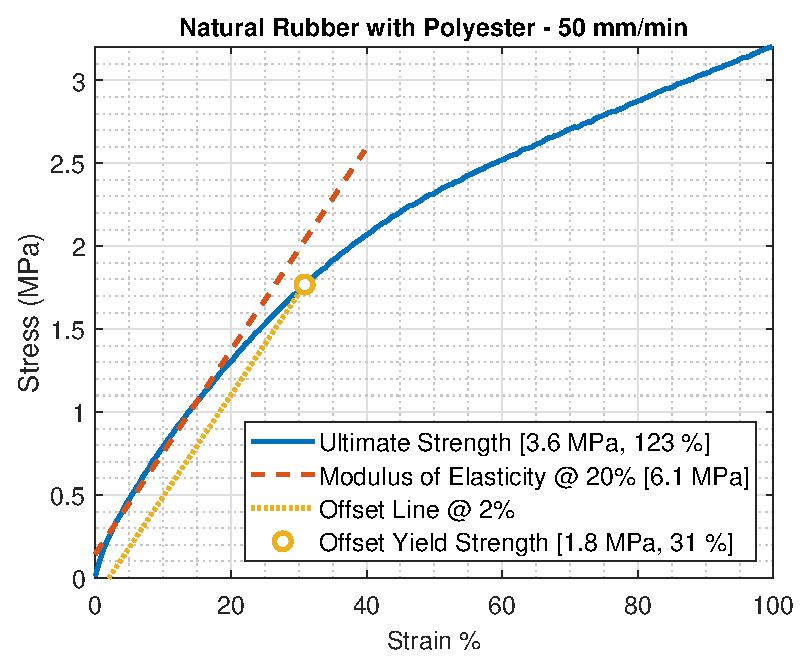
\includegraphics[width=\textwidth]{NatR_disR50.eps}
        \caption{Caption}
        \label{fig:FR250}
    \end{subfigure}
    \hfill
    \begin{subfigure}[b]{0.49\textwidth}
        \centering
        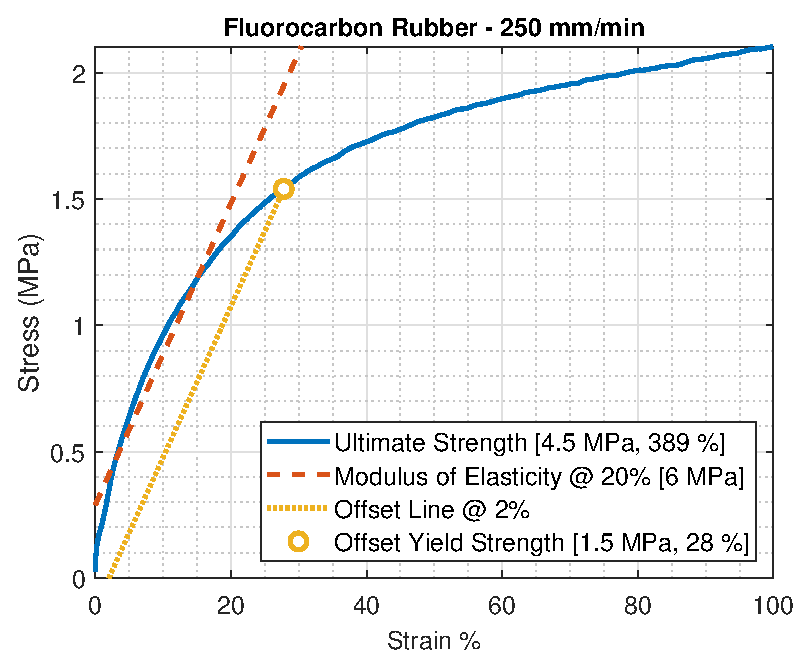
\includegraphics[width=\textwidth]{FR_disR250.eps}
        \caption{Caption}
        \label{fig:FR500}
    \end{subfigure}
    \hfill
    \begin{subfigure}[b]{0.49\textwidth}
        \centering
        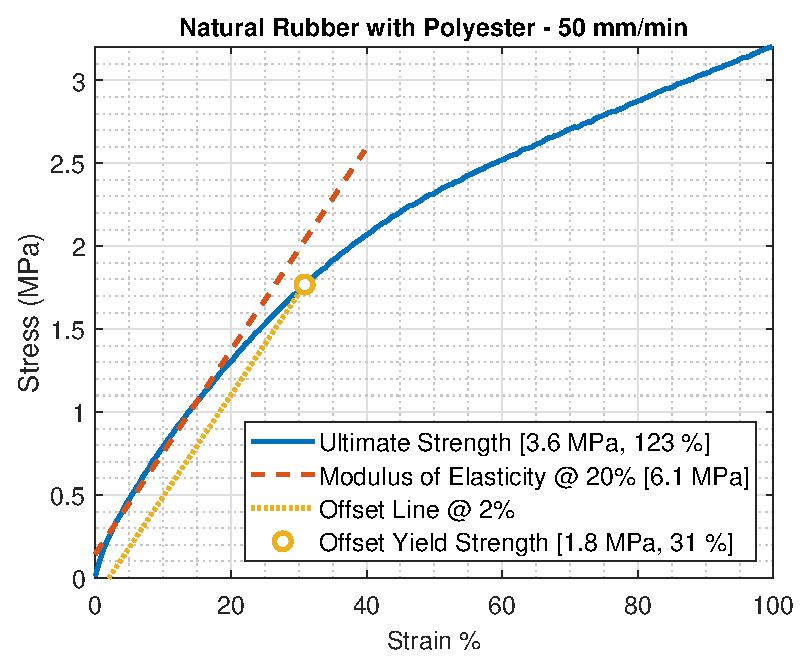
\includegraphics[width=\textwidth]{NatR_disR50.eps}
        \caption{Caption}
        \label{fig:NatR50}
    \end{subfigure}
    \hfill
    \begin{subfigure}[b]{0.49\textwidth}
        \centering
        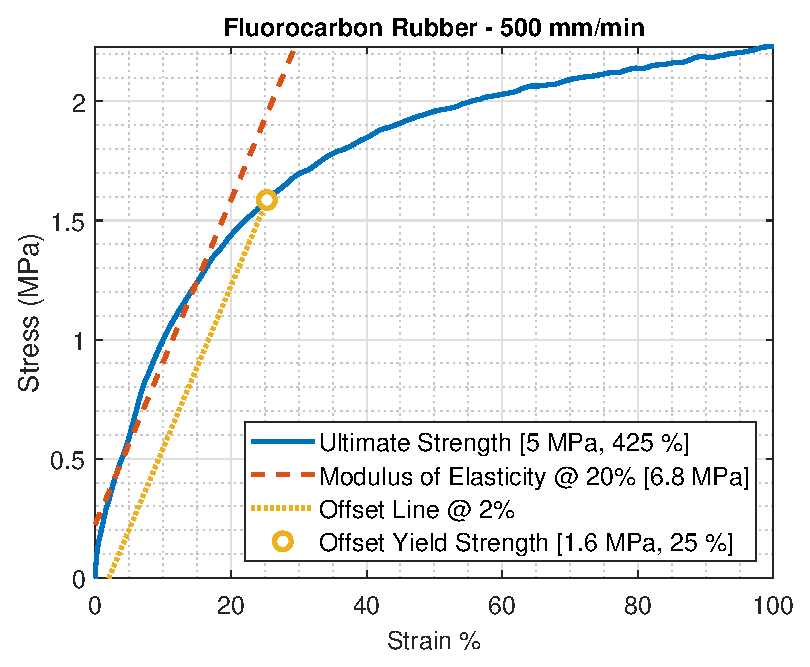
\includegraphics[width=\textwidth]{FR_disR500.eps}
        \caption{Caption}
        \label{fig:NatR250}
    \end{subfigure}
    \hfill
    \begin{subfigure}[b]{0.49\textwidth}
        \centering
        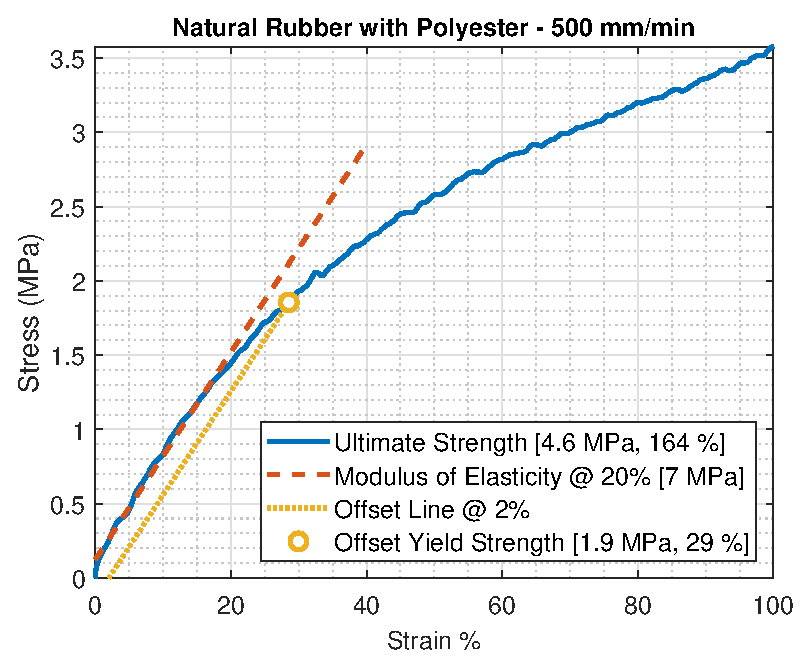
\includegraphics[width=\textwidth]{NatR_disR500.eps}
        \caption{Caption}
        \label{fig:NatR500}
    \end{subfigure}
    \caption{Caption for main figure}
    \label{fig:FRandNatR}
\end{figure}

\begin{figure}[H]
    \centering
    \begin{subfigure}[b]{0.49\textwidth}
        \centering
        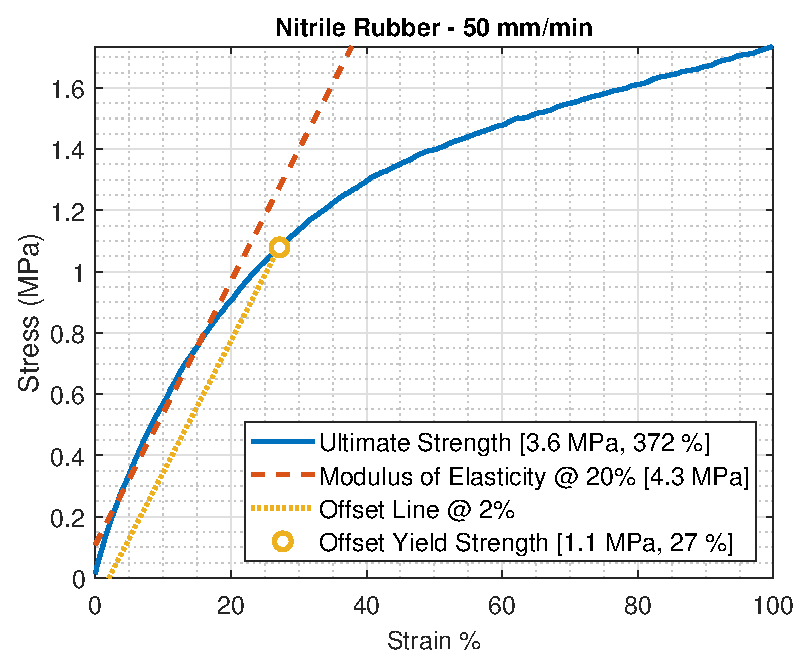
\includegraphics[width=\textwidth]{NR_disR50.eps}
        \caption{Caption}
        \label{fig:NR50}
    \end{subfigure}
    \hfill
    \begin{subfigure}[b]{0.49\textwidth}
        \centering
        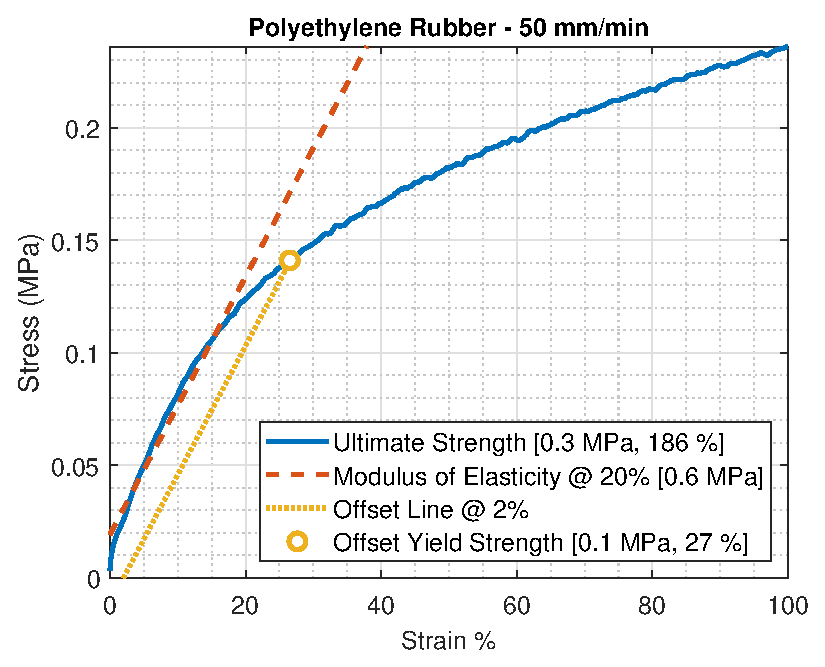
\includegraphics[width=\textwidth]{PR_disR50.eps}
        \caption{Caption}
        \label{fig:NR250}
    \end{subfigure}
    \begin{subfigure}[b]{0.49\textwidth}
        \centering
        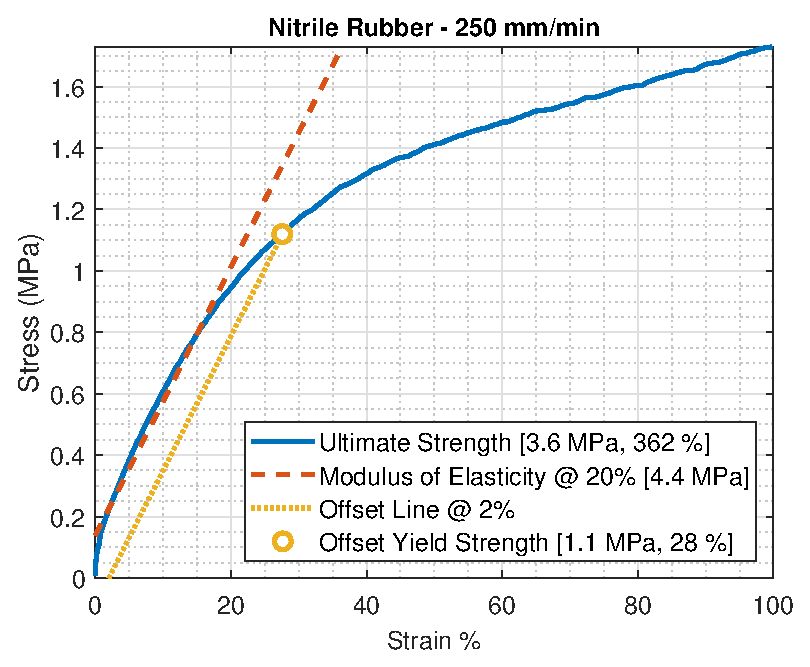
\includegraphics[width=\textwidth]{NR_disR250.eps}
        \caption{Caption}
        \label{fig:NR500}
    \end{subfigure}
    \hfill
    \begin{subfigure}[b]{0.49\textwidth}
        \centering
        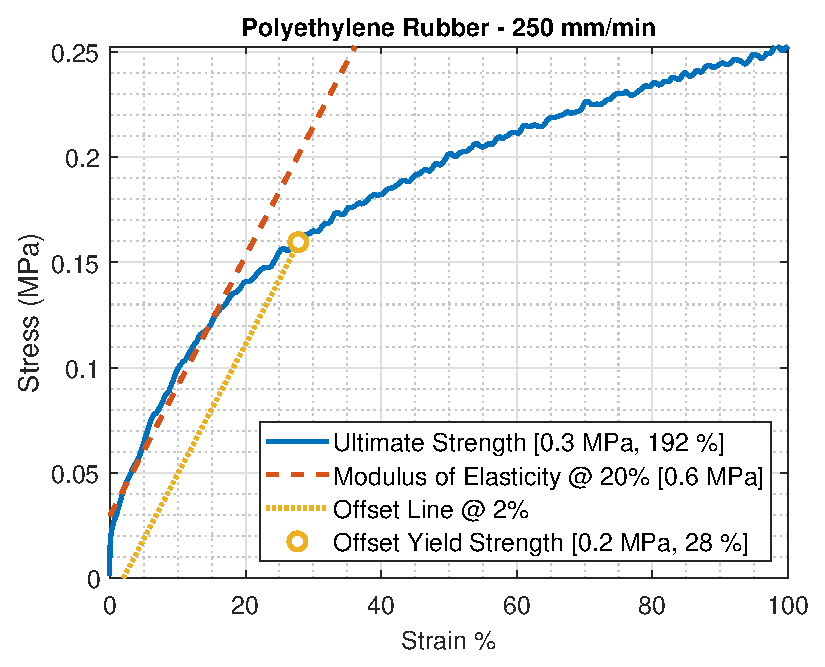
\includegraphics[width=\textwidth]{PR_disR250.eps}
        \caption{Caption}
        \label{fig:PR50}
    \end{subfigure}
    \hfill
    \begin{subfigure}[b]{0.49\textwidth}
        \centering
        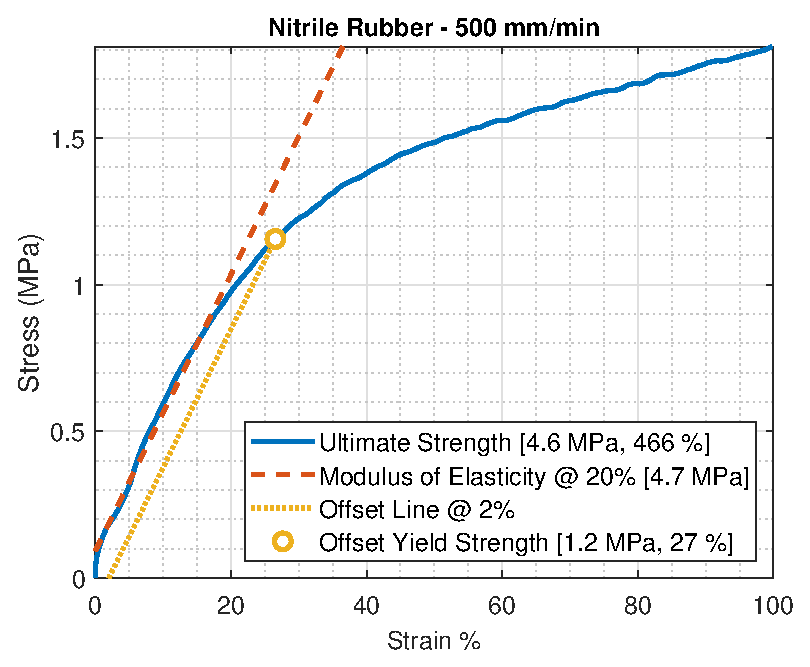
\includegraphics[width=\textwidth]{NR_disR500.eps}
        \caption{Caption}
        \label{fig:PR250}
    \end{subfigure}
    \hfill
    \begin{subfigure}[b]{0.49\textwidth}
        \centering
        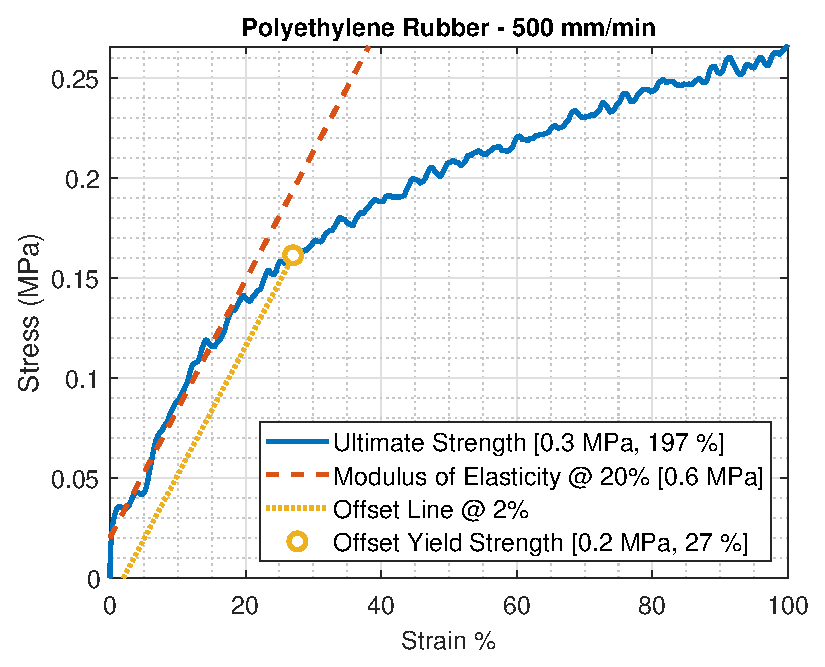
\includegraphics[width=\textwidth]{PR_disR500.eps}
        \caption{Caption}
        \label{fig:PR500}
    \end{subfigure}
    \caption{Caption for main figure}
    \label{fig:NR}
\end{figure}

\begin{figure}[H]
    \centering
    \begin{subfigure}[b]{0.49\textwidth}
        \centering
        \includegraphics[width=\textwidth]{Nat100R_disR50.eps}
        \caption{Caption}
        \label{fig:Nat100R50}
    \end{subfigure}
    \hfill
    \begin{subfigure}[b]{0.49\textwidth}
        \centering
        \includegraphics[width=\textwidth]{SR_disR50.eps}
        \caption{Caption}
        \label{fig:SR50}
    \end{subfigure}
    \hfill
    \begin{subfigure}[b]{0.49\textwidth}
        \centering
        \includegraphics[width=\textwidth]{Nat100R_disR250.eps}
        \caption{Caption}
        \label{fig:Nat100R250}
    \end{subfigure}
    \hfill
    \begin{subfigure}[b]{0.49\textwidth}
        \centering
        \includegraphics[width=\textwidth]{SR_disR250.eps}
        \caption{Caption}
        \label{fig:SR250}
    \end{subfigure}
    \hfill
    \begin{subfigure}[b]{0.49\textwidth}
        \centering
        \includegraphics[width=\textwidth]{Nat100R_disR500.eps}
        \caption{Caption}
        \label{fig:Nat100R500}
    \end{subfigure}
    \hspace*{\fill}
    \caption{Caption for main figure}
    \label{fig:Nat100R}
\end{figure}

\begin{figure}[H]
    \centering
    \begin{subfigure}[b]{0.49\textwidth}
        \centering
        \includegraphics[width=\textwidth]{EPR_disR50.eps}
        \caption{Caption}
        \label{fig:EPR50}
    \end{subfigure}
    \hfill
    \begin{subfigure}[b]{0.49\textwidth}
        \centering
        \includegraphics[width=\textwidth]{EPR_disR500.eps}
        \caption{Caption}
        \label{fig:EPR500}
    \end{subfigure}
    \caption{Caption for main figure}
    \label{fig:EPR}
\end{figure}

%Specimen Length used in the file Materials Properties has to be updated to 33 instead of 25
\begin{table}[ht!]
    \centering
    \begin{tabular}{c|c}
         &  \\
         & 
    \end{tabular}
    \caption{Caption}
    \label{tab:my_label}
\end{table}

crystallization of some materials

CRITICAL - The strain-stress curve for elastomers does not have a toe and elastic region. The effects are different and must be explained before describing the mechanical tests. Everything is summarized in Bauman's paper. More reading on the stress relaxation part is a must because I initially used the elastic region as a way to avoid plastic deformation. This can be better justified by the need of avoiding high strains to prevent chain ruptures. The first cycle of stress relaxation is the most important. More literature is required to support this. Also, crystallization explains the steep increase (stiffening) at the end of the curve in some of the rubbers I have. This chapter needs a rewriting. Moreover, plots with toe and elastic regions are no longer needed. Instead, plots showing the data from different strain rates of the same material are more suitable. The idea of training a neural network to predict the stiffness in real time is still viable. Van der Waals effects are important.

\subsection{Stress Relaxation Test}

The stress relaxation test allows the extraction of the viscoelastic (time-dependant) properties of the materials. During this test, the specimens are extended to a certain elongation level (initial strain) and are held in this position during a large period of time while the decreasing reacting force is observed. The guidelines for this experiment can be found in the ASTM D6147 \cite{astm2002d6147}. The test duration is set to three hours (TIME CHANGED IN LATEST EXPERIMENTS), following the experimental works in the literature (Case, White and Kramer, 2015) (Delin et al., 1995). The elongation level, $\epsilon_0$, must be chosen to be inside the toe region of the materials load-elongation curve to avoid plastic deformation of the material, i.e. irreparable damage. Lastly, all materials were deformed at 500 mm/min. The main viscoelastic property of interest is the amount of stress relaxation achieved in certain amount of time. The latter is easily extracted from the stress relaxation curve of each material as illustrated in Figure 4. 

\subsection{Pre-processing of experimental data}

The test results of specimens from the same material are expected to be slightly different from one another even if they were collected from the same sheet. This variability is caused by many reasons such as the manufacturing process, temperature, and micro fissures inside the material due to handling. The latter highlight the necessity of the pre-processing stage to be performed.

The raw data obtained from the Instron testing must be pre-processed before using it for any fitting process due to the unavoidable noise embedded into the data mainly due to the machine's load cell resolution. According to REFERENCE, the very first data points must be discarded, more specifically, the useful data starts from the point in which the machine has reached the desired initial deformation and remain there for a couple of seconds. In addition to this initial filtering step, the noise embedded in the data must be removed. 

Smoothing algorithms such as moving average, Gaussian weighted average, etc. are commonly implemented to clean noisy data. Matlab provides an built-in function smoothdata specifically for the latter task. This function has a selection of different smoothing algorithms. To choose the most suitable algorithm for my data I performed a comparison analysis including three different algorithms: moving average, Gaussian-weighted moving average and Savitzky-Golay filter. I observed the ability of each algorithm to smooth the noisy data by varying the size of the window in which the averaging takes place. The Gaussian-weighted moving average and Savitzky-Golay filter were the two best algorithms to smooth the raw data. However, the Gaussian-weighted moving average had the limitation of affecting greatly the maximum data value, i.e. the maximum stress obtained at the beginning of the stress relaxation test. Therefore, the Savitzky-Golay filter was selected as the best smoothing algorithm. The window size was selected using the percentage drop in the maximum stress value. The latter two parameters had a proportional relationship, i.e. the larger the window size, the larger the drop of the maximum stress value.



The filtering of the raw data was achieved following these steps:
\begin{itemize}
    \item Data beyond the failure point was ignored for all the different specimens
    \item The data from the N specimens was averaged into a single variable
    \item The failure point is different for each specimen which cause abrupt steps to be included in the averaged data. Therefore, the last 30\% of the data (chunk of data close to failure point) was scanned to find abrupt changes in the load. Abrupt changes are all changes greater than 1\% of the relative change of the current load, as described in the following equation:
    \begin{equation}
        (Load(i) - Load(i+1) ) / Load(i) * 100
    \end{equation}
    \item All NaN values are filtered from the data
    \item Make sure data does not contain initial negative values. This represent a negative offset which must be compensated to the actual experimental data
    \item The proper window size to use in the smoothing algorithm is defined. The criteria is based on the second derivative of the load-displacement curve. The effect of the window size width on the oscillation of the second derivative was analyzed to locate a section in which to search for the window size width which approaches the most to the mean value of the second derivative.
    \item Similarly as the raw data the smoothed data should not contain negative values. Making the first data point zero is too abrupt, removing the negative offset is more suitable.
\end{itemize}

The experimental data obtained from the tests is processed in Matlab to filter out any undesired noise and misreadings. As previously mentioned, a total of five specimens per material are subjected to the same test. The first step in processing the data is to compile these five sets of data into a single one by averaging them together. The next step is to remove any undesired offset from the resulting data set which ensures that the stress-strain curve begins from zero as desired. Lastly the data a smoothing algorithm based on the 

\section{Comparison Analysis - INCOMPLETE}

\subsection{Tensile Strength Test}

Finally, the mechanical properties of the human quadriceps tendon (Schatzmann, Brunner and St{\"a}ubli, 1998) and of the six soft materials are compiled and compared in ADDTABLE. In this table, the difference between the cross-sectional area of the human tendon and the materials is highlighted and reflected in the difference between their mechanical properties. However, even by matching the human tendon cross-sectional area, the current soft materials are not able to match its strength. The latter is discussed in detail in section 3.

\subsection{Stress Relaxation Test}

In the literature, stress relaxation experiments on the human patellar tendon have been performed (Johnson et al., 1994). The tests duration in this work is 300 seconds which differs from the three hours of our experimental setup. Therefore, the materials and the human tendon are compared on the time frame of 300 seconds. The achievable amount of stress relaxation is defined by Eq. (1) as follows:

Where achieved stress relaxation at the 300 seconds mark,  and  are the initial and final stress, respectively. 

Lastly, the data from the human patellar tendon is compared against the materials data in Table II.

In contrast with the great difference observed between the elastic properties of the soft materials and the human tendon (Table I), the viscoelastic properties of the soft  extracted from the stress relaxation tests are closer to the human tendon ones. These results are discussed in detail in Section 3.


{\huge The Best Candidate Explanation}

At this stage, the elastic and viscoelastic properties of the soft materials and the human tendon have been compared against each other. The results highlights that the Flourocarbon Rubber  has the most similarities to the human tendon mechanical properties. This is based on the two tables summarizing the elastic and viscoelastic properties of both.
To-do List
\begin{itemize}
    \item Define the criteria to choose which material is the most suitable
    \item Elastic parameters
    \begin{itemize}
        \item Stiffness at Toe region (small deformation)
        \item Stiffness at Elastic region (long deformation)
        \item Ultimate load
        \item Ultimate elongation
        \item Matching Factor(increment factor of the material cross-sectional area required to match the human tendon strength)
        
    \end{itemize}
    \item Viscoelastic parameters
    \begin{itemize}
        \item 
    \end{itemize}
\end{itemize}



\section{Summary}
\chapter{Soft Materials Modelling: Linear Viscoelastic Models}

\section{Introduction}

\chapter{Soft Materials Modelling: Neural Networks}

\section{Introduction}

This is the last part to write. The chapter will include the following:

\begin{itemize}
    \item (Introudction) Reintroduce the problematic when using model-driven approaches such as mathematical models for this application. Then, mention the current research focused on neural networks as a potential solution.
    \item Theory and definition of a neural network (NN)
    \item Literature focused on NNs. Mention relevant applications and their methodology.
    \item Method1: Describe the methodology used for the systematic approach of a single material (Maybe include all of them in one go)
    \item Results1: Discuss obtained performance
    \item Method2: Select best topologies and apply those to the other materials. Mention the specific case of the rubber bands with different thickness
    \item Results2: Discuss the obtained performance
    \item Simulink validation. This step will justify the needs of a experimental work. The main objective of this section is to analysis the performance of NN in real-time when implemented as part of a control system
\end{itemize}

\subsection{Work history}
\begin{itemize}
    \item 15/May/18: First mention of Artificial Neural Networks as a way to predict the complex behaviour of the soft materials of interest. The latter is motivated by the limitations of the complex mathematical model and fitting process. The first step was to use Matlab to quickly test the performance of simple feedforward networks using the raw data from the tensile strength experiments.
    \item 17/May/18: Simple preliminary tests shows promising results. The following is required: 
    \begin{itemize}
        \item Understand the motivation of using neural networks (quicker, robust and simpler way to model a complex behaviour).
        \item Define network inputs/outputs.
        \item Perform detailed literature review on the implementation of neural networks for characterization of materials.
    \end{itemize}
    \item Check logbook pages at meeting of 17/May/18 for summary of the literature review performed and Google Scholar search parameters.
    \item The most relevant work found was dated from 2015 and titled ``Prediction of stress relaxation for rubber composites''. An improved radial basis function (RBF) is used to predict the stress relaxation curve of rubbers.
    \item 12/Jun/18 Task: Review 2015 paper on ANN for rubbers.
    \item 10/Jul/18 Meeting highlights: 
    \begin{itemize}
        \item Perform extra tensile strength experiments to increase the current set of data, potentially improving the neural network response. 
        \item Journal Paper (Modelling): The work done on the viscoelastic mathematical models and the artificial neural networks can be compiled into a good journal paper.
    \end{itemize}
    Tasks:
    \begin{itemize}
        \item Review literature and base on it the experimentation being done on ANN
        \item Identify the soft material (Silicone Rubber) for which the mathematical model yielded the highest error (worst performance).
        \item Test the performance of different neural networks architectures on the identified soft material.
    \end{itemize}
    \item Important Notes - Most used neural networks architectures for prediction of materials' properties
    \begin{itemize}
        \item Supervised Networks
        \begin{itemize}
            \item Feedforward Networks
            \begin{itemize}
                \item Backpropagation
                \item Perceptron
            \end{itemize}
            \item Radial Basis Function
            \begin{itemize}
                \item Genetic Algorithm
                \item Bare-bone Particle Swarm Optimization
            \end{itemize}
        \end{itemize}
    \end{itemize}
    \item First Formal Experimentation 
    \begin{itemize}
        \item Dataset - In the literature, the data from 20 different experiments (on average) is used for the training of neural networks. In accordance with this, there is not enough data to properly test the performance of the neural networks. However, we decided to move forward and test the neural networks using the following:
        \begin{itemize}
            \item Ethylene Polypropylene Rubber (EPR): 5 sets
            \item Flourocarbon Rubber (FR): 8 sets
            \item Natural Rubber (NatR): 7 sets
            \item Nitrile Rubber (NR): 7 sets
            \item Polyethylene Rubber 6mm (PR): 7 sets
            \item Silicone Rubber (SR): 8 sets
        \end{itemize}
        \item Parameters:
        \begin{itemize}
            \item Network achitecture: feedforward backpropagation
            \item Number of hidden layers: 1
            \item Number of neurons in the hidden layer: 10
            \item Inputs: strain and strain rate
            \item Output: stress
            \item Data: Raw data used, data beyond the ultimate load is discarded to increase prediction accuracy
        \end{itemize}
        \item Results
        \begin{itemize}
            \item Comparison Analysis (documented in StressResponse.png and StressResponseFull.png):
            \begin{itemize}
                \item Raw Data Neural Networks
                \item Preprocessed Data Neural Networks
                \item Preprocessed Data Mathematical Model
            \end{itemize}
        \end{itemize}
    \end{itemize}
    \item 17/Jul/18 Meeting Highlights:
    \begin{itemize}
        \item Train neural network with preprocessed data
        \item At this point, only feedforward architecture has been tested. Radial Basis Function must also be tested
    \end{itemize}
    \item 18/Jul/18 Meeting Highlights:
    \begin{itemize}
        \item Focus on obtaining the performance (mean squared error) of the neural networks when different numbers of neurons are used in the hidden layer
        \item Certain parameters must be considered when assessing the performance of neural networks, such as momentum and learning rate
        \item The performance of neural networks can be analyzed in a shorter deformation range in accordance to the application (activities of daily living, knee) we are interested in. This can also result in better performance and faster training times.
        \item First exploration to perform and observe the behaviour of the neural networks: number of neurons (increase to 15)
        \item Uriel's suggestion: Recurrent Neural Networks
    \end{itemize}
    \item Important Notes - Exploration progress is documented in the logbook after the meeting of 18/Jul/18. The many tests performed are detailed in there. In summary:
    \begin{itemize}
        \item The analysis regarding the effect of varying the number of neurons in the hidden layer highlighted an ideal range in which the best performance (lowest mse) is obtained. Overall, less than 10 neurons are required to obrain a good generalization.
        \item Adding a second hidden layer has no meaningful effect on the performance of feedforward networks.
        \item A data division of [80,10,10] for training, test and validation, respectively, was suitable for these networks. The recommended spread is [70,15,15] which was also tested
        \item Multiple training sessions were performed on the networks with best performance to increase their generalization capabilities, as recommended in the literature.
        \item The neural networks performance was assessed for two scenarios: full range, and elastic region of stress-strain curve. The effect of adding a second hidden layer and performing multiple training sessions is more noticeable in the elastic region scenario.
    \end{itemize}
    \item Important Notes - Feedforward Back-propagation networks have proven useful for modelling of the soft materials. However, other architectures such as Recurrent Neural Networks might perform even better. This needs to be investigated.
    \item 31/Jul/18
    \item 4/Aug/18
    \item Simulink analysis
    \begin{itemize}
        \item The first attempt to compare the performance of the neural networks when modelling the elastic element of a series-elastic actuator was UNSATISFACTORY. I focused on investigating the latter. Potentially, the fact that the elastic element can only be modelled under tension was not described properly in Simulink. Another possibility is the fact that the data used to train the neural networks is slightly different than the one used for the mathematical model.
        \item The transfer function was originally defined to take the material's deformation as input. In a real application, the material's deformation will be measured and use as an input to estimate the material's force.
        \item Following the previous note. The behaviour of the material when the pulling force deforming it disappears must be investigated. This invert the current relationship analyzed where the deformation is considered as an input of the model. In a real application, a motor will create a pulling force to deform the material, this force must be used to calculate the material's deformation. This approach might be completely out of place since the main reason of using series elastic element (control-wise) is to simplify the control itself. This means that the deformation of the material is the only one required to be measured to estimate the material's force.
        \item This analysis needs to be done again focusing on the soft material with best performance to make the process quicker.
    \end{itemize}
    \item 18/Feb/119 - Second Exploration performed
    \begin{itemize}
        \item In this stage we are assuming that the mathematical model is not able to predict a material's behaviour in a general way. This is the main justification for using neural networks since these can generalize the material's behaviour if trained correctly. The mathematical model has been tested when using plenty of strain segments in the piecewise linearization process, the more segments are used the less generalization is able to be obtained from the model. There must be a way to obtain the right number of strain segments which avoid over-fit. The latter is the best way to compare the neural network performance against the model.  
        \item The best materials so far is the Flourocarbon Rubber, according to the paper presented in Innovationmatch MX (this needs to be reviewed). The following validation must be based on this material only, to quicken the process of proving the concept. 
    \end{itemize}
    
\end{itemize}

\section{Artificial Neural Networks}

In the previous chapter, the computational cost of using mathematical models for modelling the behaviour of soft materials is highlighted. Recently, research is being focused on using machine learning tools, such as artificial neural networks (ANNs), as an alternative to the traditional Linear Viscoelastic Models (LVMs) for modelling the mechanical behaviour of soft materials. In the literature, ANNs has demonstrated high accuracy when characterizing different mechanical phenomenons found in soft materials, such as, stress relaxation, nonlinear stress-strain response, temperature  and time dependency, to mention a few.

The next paragraph will describe the works being done on stress-strain curve prediction. Finalizing with other applications. These are the relevant papers:

\begin{itemize}
    \item Stress-strain
    \begin{itemize}
        \item Prediction of the tensile response of carbon black filled rubber blends by artificial neural network
        \item Viscoelastic analysis of a sleeve based on the BP neural network
        \item Use of artificial neural network for prediction of physical properties and tensile strengths in particle reinforced aluminum matrix composites
    \end{itemize}
    \item Stress Relaxation
    \begin{itemize}
        \item Prediction of nonlinear viscoelastic behavior of polymeric composites using an artificial neural network
    \end{itemize}
    \item Different Mechanical Properties
    \begin{itemize}
        \item Predicting mechanical properties of elastomers with neural networks
    \end{itemize}
\end{itemize}

To do list:
\begin{itemize}
    \item Develop Matlab algorithm to assess the performance of the proposed topologies based on the three steps optimization done in one of the papers above
    \begin{itemize}
        \item Retrain neural network for the Natural Rubber material using a slightly different training set. Extract one test dataset from each strain rate and don't include this in the training set.
    \item During training, store the achieved mse performance and the R coefficient during training, testing and validation for each neuron combination.
    \item Finally, calculate the mse performance of the trained network using the unknown dataset
    \item Make sure to store the previous information inside the final mat-file using proper variables to allow the plotting of this information in a different section.
    \end{itemize}
\end{itemize}

Introduction Paragraph: Important Question: In the field of implementing neural networks for the prediction of the stress-strain curve of soft materials, What are the most common topologies used? This is the base line for this chapter and the systematic analysis of testing different topologies of neural network.

IDEA: The analysis of the performance of the neural network can be justified by using the piecewise linearization model. The right combination of strains segments and of parallel springs must be selected to comply with the following three optimization aspects: 1. Minimal mean square error 
2. Maximal linear correlation coefficient R for the available strain rates, simultaneously
The latter might require something else than a simple algorithm. In that case, when a proper optimization algorithm is required, such as GA, this idea is might not be in the scope of this project.


Things to explain in this section:
\begin{itemize}
    \item Mathematical definition of a Neural Network
    \item Literature implementing Neural Networks for modelling of soft materials
    \item Multilayer Perceptron (MLP). Some information available in \cite{aulova2017determination} page 337.
    \item Radial Basis Function (RBF). This is a feedforward neural network which utilizes the radial-basis activation function in its hidden layer, and it only has one hidden layer, \cite{aulova2017determination}.
\end{itemize}

\subsection{Description of the systematic approach chosen to test the different topologies of NNs} 
 In this section I will discuss about the relevant work done on modelling soft materials (elastomers) using neural networks
 
\subsubsection{The very first comparison analysis}

Initially I trained several neural networks, which were only able to recognize one out of three displacement rate, because they were only trained with that data. Therefore, this networks were not able to predict the stress-strain curve of the material for different displacement rates apart from the one used for training. This limitation was also exhibited in the mathematical model.

This findings directed us towards attempting to train the neural networks to be able to recognize all displacement rates of the material, hence, being able to account for the strain dependency of the stress-strain curve of elastomers.

The latter has to be documented, I used a totally different database as the one I am using now. But the comparison analysis justifies the path taken towards retraining the neural networks.

Analysis explanation: The paper "Artificial neural network model for material characterization by indentation" has a very good example on how to present the neural networks that you have implemented, on page 1059. 

\subsection{Measures of modelling performance}
 
In this paragraph I am going to summarize the different metrics used in the literature when assessing the performance of neural networks.

Introduction Paragraph: The performance of a neural network for regression applications is assessed in two main parts, by analyzing the difference between the neural network prediction and the experimental data, and by analyzing the percentage of correct predictions. The former analysis refers to the neural network prediction error, which can be assessed by different statistical parameters. These are the ones most mentioned in the literature: mean square error (MSE), root mean square error (RMSE), the average relative error (AVE), the sum of square of errors (SSE), the mean absolute error (MAE), the standard deviation normalized root mean square error (NRMSE). 

The preference between one parameter and the other is dependent on the type of application. (explain the main difference between these statistical measurements). This suggest filtering the references to include only the ones using a principal component analysis and the ones using the raw data itself.

The latter analysis refers to the coefficient of determination, also known as R-squared ($R^2$). \cite{aulova2017determination,tho2004artificial,saha2018use,setti2014artificial,xu2019application}. 

Pending: Get the bibtex version of the other relevant papers using neural networks for prediction of mechanical properties of soft materials. The list needs to be filtered to focus on viscoelastic cases, and mention a few other close-related cases

In this work, the main objective is to design and train neural networks able to predict the mechanical behaviour of soft materials during different strain or deformation rates. Therefore, the performance of the neural network is desirable to be similar in all different cases and avoid favouring the prediction of a specific strain rates.



MSE and R2 papers:

\begin{itemize}
    \item The Determination of relaxation modulus of time-dependent materials using neural networks, \cite{aulova2017determination}: This paper is from 2016, and the author states that there are practically no papers addressing the NN modelling of the behaviour of viscoelastic materials. The author also states that using data from experimental tests carry unavoidable errors and that this is considered an ill-posed problem. This work focuses on the stress relaxation curve of a material, a behaviour that can be approximated very well using generalization or parametric regression methods, such as the nonlinear parametric regression. The prediction of the NNs studied in here are compare against such models. The topologies of NNs studied in this work are the Multilayer Perceptron and the Radial Basis Funtion, both of which are considered as universal function approximators. In this work, two parameters are used to assess the performance of the neural networks: the MEAN SQUARE ERROR AND THE R0.95 (\%). In addition to this, the performance was assessed taking into consideration the capabilities of the neural networks in this three aspects: generalization, robustness and mathematical convergence.
    \item The paper: Use of an Artificial Neural Network Approach for the Prediction of Resilient Modulus for Unbound Granular Material, make use of the MSE and the coefficient of determination R2 (CITED)
    \item The paper: Artificial neural network approach for prediction of stress-strain curve of near titanium alloy, make use of the MSE, the coefficient of determination and the Average Relative Error (ARE) (CITED)
    \item The paper: Artificial neural network model for material characterization by indentation, make use of the MSE (CITED)
    \item The paper: Application of radial basis neural network to transform viscoelastic to elastic properties for materials with multiple thermal transitions, make use of the root mean square error to asses the performance of the proposed networks.
\end{itemize}

The paper: Predicting mechanical properties of elastomeric modified nylon blend using adaptive neuro-fuzzy interference system and neural network, make use of the R2 coefficient and the Root Mean Square Error (RMSE)

The paper: Comparative analysis of feed forward and radial basis function neural networks for the reconstruction of noisy curves, make use of the Sum of Square of Errors (SSE)

The paper: Predicting mechanical properties of elastomers with neural networks, make use of the RMSE normalized to the standard deviation (NRMSE), the Mean Absolute Percentage Error (MAPE) and the percentage of correctly classified samples (not applicable for my work)

The paper: Radial Basis Function Neural Network-Based Modeling of the Dynamic Thermo-Mechanical Response and Damping Behavior of Thermoplastic Elastomer Systems, make use of the MSE.

The paper: Application of radial basis neural network to transform viscoelastic to elastic properties for materials with multiple thermal transitions, make use of the Root Mean square Error (RMSE)

The paper Viscoelastic analysis of a sleeve based on the BP neural network, make use of MSE. Review this paper because it has important theory about the generalization of neural networks depending on the error during training and during validation

This paper is the oldest regarding the implementation of Neural Networks for prediction of the viscoelastic behaviour of composite materials: Prediction of nonlinear viscoelastic behavior of polymeric composites using an artificial neural network. I have to review this carefully.
\chapter{Conclusions}

\section{Introduction}

This chapter focuses on assessing the mapping capabilities of neural networks when implemented in a control system. Moreover, the benefits of using a soft materials as the elastic element in a series-elastic actuator is assessed by comparing it against the traditional series-elastic actuator with a metallic spring.

\section{Traditional Series-elastic Actuator Model}

OBJECTIVE: Document the process in which the transfer function of the system is deducted, firstly for a traditional motor-load system, then for a traditional SEA and finally, for a soft SEA.

The process for modelling single robotic joint, based on an electric motor, is described in the book "Robotics: Control, Sensing, Vision, and Intelligence" from K.S. Fu. The dynamic behaviour of an electric motor can be defined by two constitutive equation, one for the electric part and other for the mechanical part of the motor. Following Kirchhoff voltage rule and Newton's second law we obtain the two following equations:



\appendix
\begin{appendix} 
\chapter{Characterization of the Human Body Lower Limb} \label{appendixA}
This appendix presents the reviewed clinical studies for four main human activities of daily living: walking, ascending/descending steps, ascending/descending ramps and sitting down/standing up from chair. The compilation of data was performed to characterize the relevant parameters for the motion of human lower limb. From the clinical trials it was taken the angle, torque and power of each joint for the lower limb, i.e. hip, knee and ankle. Subsequently, the data was compiled into a table and then into several charts which focused on representing the range of motion of each joint during each activity.
\end{appendix}

%\begin{appendix}
\chapter{Appendix New} \label{appendixB}


\end{appendix}
%. More appendicies here.
\addcontentsline{toc}{chapter}{References} % Adds References to contents page
\bibliographystyle{unsrtnat} % bibliography style
\renewcommand{\bibname}{References} 
\bibliography{References/Bibliography} % References file
\end{document}